\documentclass[UTF8]{pkuthss}

\usepackage[backend = biber, style = caspervector, utf8, sorting = ecnty]{biblatex}
\usepackage{amssymb}
\usepackage{amsmath}
\usepackage{graphicx}
\usepackage{deluxetable}
\usepackage{color}
\usepackage{bm}

\setlength{\bibitemsep}{3bp}
\renewcommand*{\bibfont}{\zihao{5}\linespread{1.27}\selectfont}

\pkuthssinfo{
	cthesisname = {硕士研究生学位论文}, ethesisname = {Master Thesis},
	ctitle      = {基于近场动力学理论的弹塑性材料形变及碎裂仿真},
    etitle      = {Peridynamics-Based Deformation and Fracture Animation for Elastoplastic Solids},
	cauthor     = {陈伟},
	eauthor     = {Wei Chen},
	studentid   = {1501214372},
	date        = {二〇一八\ 年\ 六\ 月},
	school      = {信息科学技术学院},
	cmajor      = {计算机软件与理论},
    emajor      = {Computer Software and Theory},
	direction   = {计算机图形学},
	cmentor     = {李胜\ 副教授},
    ementor     = {Sheng Li},
	ckeywords   = {近场动力学,形变,碎裂,弹塑性, 仿真},
    ekeywords   = {peridynamics, deformation, fracture, elastoplasticity, animation}
}

\addbibresource{thesis.bib}

\begin{document}

    \newcommand{\xii}{\textbf{x}_i}
\newcommand{\xj}{\textbf{x}_j}
\newcommand{\vi}{\textbf{v}_i}
\newcommand{\vj}{\textbf{v}_j}
\newcommand{\fin}{\textbf{f}_i^{int}}
\newcommand{\fex}{\textbf{f}_i^{ext}}

\newcommand{\X}{\textbf{X}}
\newcommand{\Y}{\textbf{Y}}
\newcommand{\Z}{\textbf{Z}}
\newcommand{\F}{\textbf{F}}
\newcommand{\E}{\textbf{E}}

\newcommand{\mb}[1]{\mathbf{#1}}

\newcommand{\bfT}{\textbf{T}}
\newcommand{\bft}{\textbf{t}}
\newcommand{\bfu}{\textbf{u}}
\newcommand{\bfx}{\textbf{x}}
\newcommand{\bff}{\textbf{f}}
\newcommand{\bfv}{\textbf{v}}
\newcommand{\bfy}{\textbf{y}}
\newcommand{\bfui}{\textbf{u}_{(i)}}
\newcommand{\bfvi}{\textbf{v}_{(i)}}
\newcommand{\bffi}{\textbf{f}_{(i)}}
\newcommand{\bfyi}{\textbf{y}_{(i)}}
\newcommand{\bfuj}{\textbf{u}_{(j)}}
\newcommand{\bfxi}{\textbf{x}_{(i)}}
\newcommand{\bfxj}{\textbf{x}_{(j)}}
\newcommand{\bfyj}{\textbf{y}_{(j)}}
\newcommand{\bfvj}{\textbf{v}_{(j)}}
\newcommand{\bfxl}{\textbf{x}_{(l)}}
\newcommand{\bfyl}{\textbf{y}_{(l)}}
\newcommand{\bfuk}{\textbf{u}_{(k)}}
\newcommand{\bfxk}{\textbf{x}_{(k)}}
\newcommand{\bfyk}{\textbf{y}_{(k)}}
\newcommand{\wij}{\omega_{(i)(j)}}
\newcommand{\wkj}{\omega_{(k)(j)}}
\newcommand{\wkl}{\omega_{(k)(l)}}
\newcommand{\skj}{s_{(k)(j)}}
\newcommand{\skl}{s_{(k)(l)}}
\newcommand{\fkj}{\textbf{f}_{(k)(j)}}
\newcommand{\tkj}{\textbf{t}_{(k)(j)}}
\newcommand{\tjk}{\textbf{t}_{(j)(k)}}
\newcommand{\thetai}{\theta_{(i)}}
\newcommand{\thetak}{\theta_{(k)}}

\newcommand{\mycite}[2]{\textcolor{blue}{(#1 et al. #2)\parencite{#1#2}}}
\newcommand{\myciteTwo}[3]{\textcolor{blue}{(#1 et al. #2\parencite{#1#2},#3\parencite{#1#3})}}
\newcommand{\myciteThree}[4]{\textcolor{blue}{(#1 et al. #2\parencite{#1#2},#3\parencite{#1#3},#4\parencite{#1#4})}}
\newcommand{\fa}{${}^{\textrm{a}}$}
\newcommand{\fb}{${}^{\textrm{b}}$}




	\frontmatter
	\pagestyle{empty}
	\maketitle
	\cleardoublepage

	% Copyright (c) 2008-2009 solvethis
% Copyright (c) 2010-2017 Casper Ti. Vector
% All rights reserved.
%
% Redistribution and use in source and binary forms, with or without
% modification, are permitted provided that the following conditions are
% met:
%
% * Redistributions of source code must retain the above copyright notice,
%   this list of conditions and the following disclaimer.
% * Redistributions in binary form must reproduce the above copyright
%   notice, this list of conditions and the following disclaimer in the
%   documentation and/or other materials provided with the distribution.
% * Neither the name of Peking University nor the names of its contributors
%   may be used to endorse or promote products derived from this software
%   without specific prior written permission.
%
% THIS SOFTWARE IS PROVIDED BY THE COPYRIGHT HOLDERS AND CONTRIBUTORS "AS
% IS" AND ANY EXPRESS OR IMPLIED WARRANTIES, INCLUDING, BUT NOT LIMITED TO,
% THE IMPLIED WARRANTIES OF MERCHANTABILITY AND FITNESS FOR A PARTICULAR
% PURPOSE ARE DISCLAIMED. IN NO EVENT SHALL THE COPYRIGHT HOLDER OR
% CONTRIBUTORS BE LIABLE FOR ANY DIRECT, INDIRECT, INCIDENTAL, SPECIAL,
% EXEMPLARY, OR CONSEQUENTIAL DAMAGES (INCLUDING, BUT NOT LIMITED TO,
% PROCUREMENT OF SUBSTITUTE GOODS OR SERVICES; LOSS OF USE, DATA, OR
% PROFITS; OR BUSINESS INTERRUPTION) HOWEVER CAUSED AND ON ANY THEORY OF
% LIABILITY, WHETHER IN CONTRACT, STRICT LIABILITY, OR TORT (INCLUDING
% NEGLIGENCE OR OTHERWISE) ARISING IN ANY WAY OUT OF THE USE OF THIS
% SOFTWARE, EVEN IF ADVISED OF THE POSSIBILITY OF SUCH DAMAGE.

% 此处不用 \specialchap,因为学校要求目录不包括其自己及其之前的内容。
\chapter*{版权声明}
% 综合学校的书面要求及 Word 模版来看,版权声明页不需加页眉、页脚。
\thispagestyle{empty}

任何收存和保管本论文各种版本的单位和个人,
未经本论文作者同意,不得将本论文转借他人,
亦不得随意复制、抄录、拍照或以任何方式传播。
否则一旦引起有碍作者著作权之问题,将可能承担法律责任。

% 若需排版二维码,请将二维码图片重命名为“barcode”,
% 转为合适的图片格式,并放在当前目录下,然后去掉下面 2 行的注释。
%\vfill\noindent
%\includegraphics[height = 5em]{barcode}

% vim:ts=4:sw=4




	\cleardoublepage
	\pagestyle{plain}
	\setcounter{page}{0}
	\pagenumbering{Roman}

	% Copyright (c) 2014,2016 Casper Ti. Vector
% Public domain.

\begin{cabstract}
	\pkuthssffaq % 中文测试文字
\end{cabstract}

\begin{eabstract}
	Test of the English abstract.
\end{eabstract}

% vim:ts=4:sw=4


	\tableofcontents

	\mainmatter
	\chapter{绪言}
\label{chap1_introduction}
\section{研究背景}
随着科学技术的不断向前,人们对于工程应用中的设计可靠性和虚拟应用中的真实感体验亦在不断提出更高的要求。而物理仿真作为解决此类问题的关键技术手段,在计算机硬件的不断发展和计算能力大幅度提升的背景下,近年来得以快速跨越式向前发展。

所谓基于物理的仿真是指通过对物体建立能够表征其物理属性的动力学模型,在计算机上以某种合适的方式进行离散数值计算,从而能对真实世界中的物理行为进行模拟。物理仿真在计算机科学中占据重要地位,并应用于多个不同的关键领域。例如,在基础物理领域,往往通过物理仿真来寻找其中的统计规律,揭示真实世界中的物理原理。在计算机图形学领域以及电影、游戏等工业界,物理仿真更是给用户带来高逼真度沉浸式体验的关键技术。总之,物理仿真应用具备数据密集和计算密集双重特点,其作为一项基础性技术,在电影、工程设计、游戏等产业领域应用广泛、用户众多,是国家近年来大力发展的战略性新兴领域。

形变仿真是物理仿真的重要组成部分。形变现象在生活中几乎无处不在,常见的形变体材料包括人体的肌肉组织、布料、纸张、毛发、橡胶果冻等。事实上,绝对的刚体是不存在的,物体都或多或少存在一定形变。形变体的形变行为非常复杂:拉伸、压缩、扭曲等。在工程领域,碎裂仿真是研究材料特性以及进行辅助结构设计的重要手段。不过相对于工程材料等科学领域对于仿真精确性的高要求,图形学领域的应用相对更强调系统的稳定性和视觉效果。为提高效率,往往倾向于对模型进行一定的简化以更快地得到结果。

碎裂仿真是物理仿真的另一个重要分支。在日常生活中,碎裂效果(如玻璃碎裂、爆炸等)往往给人以深刻印象。碎裂仿真是游戏动画、数字电影和工程仿真等领域的研究热点,其具有极大的应用价值。在电影特效领域,出于成本以及人员安全的考量,真实地拍摄爆炸等大规模碎裂场景往往不具有可行性。而通过高性能计算机进行碎裂仿真,不仅能够降低电影的制作成本,而且可以控制整个断裂或者碎裂的过程,还有利于艺术家的后期设计与制作。在游戏领域,碎裂现象的实时模拟更是交互的重要组成部分,是给予玩家真实游戏体验的关键要素。在国防领域,因为炸弹轰击而产生的爆炸效果也是碎裂的一种典型现象,对于爆炸效果的碎裂仿真将极其有助于研究武器的杀伤力,进行武器的设计。弹塑性物体的碎裂在生活中也随时可见,如橡胶材料的碎裂等。手术时对人体器官的切割实际上也是一种形变体碎裂,研究在虚拟手术中的人体组织器官的交互式切割仿真,可在手术演示和手术人员的操作训练起到重要辅助作用,更具有广阔的前景。

虽然近年来,物理仿真已经在学术界得到广泛研究。但至今为止,尤其对于碎裂仿真,仍然缺乏能够在计算的效率上、计算的稳定性和可靠性上以及实现的简单性上能够支撑起工业界应用的仿真方法,更为成熟的形变仿真和碎裂仿真方法亟待进一步探索。本文的目的即是从近场动力学理论出发,提出了一整套用于弹塑性材料的形变、可延展性碎裂和脆性碎裂的无网格仿真框架,为物理仿真提供新的思路。

\section{相关工作综述}
\label{related_work}

\subsection{弹塑性形变仿真}

在图形学领域,最开始的塑性形变体仿真可以追溯到 \mycite{Terzopoulos}{1988}。随后 \textcolor{blue}{(O'Brien et al. 2002)\parencite{OBrien2002}} 在 FEM 框架中引入了一个加法形式的塑性模型来模拟可延展性材料的碎裂。在其模型中,应变张量被分解为两个部分:弹性形变和塑性形变。\textcolor{blue}{(M\"{u}ller et al. 2004)\parencite{Muller2004}} 同样采用这一模型用来模拟物体的塑性行为,但这一工作是在基于粒子的无网格框架进行的。随后\mycite{Irving}{2004}在其工作中提出了一个关于塑性的乘法模型,并指出其能更好的处理塑性行为。不同于加法模型,乘法模型是将形变分解相乘的两个部分。这一模型后续被其他工作广为采用,如\mycite{Bargteil}{2007} 模拟大规模场景下的粘滞流体,\mycite{Gerszewski}{2009} 仿真弹塑性固体,\mycite{Stomakhin}{2013} 用来模拟雪的塑性等。

然而上述几乎所有的办法几乎都无法直接应用于近场动力学模型,因为在其积分表述中并不存在形变梯度或者应变张量的概念。因此,在本文中我们将呈现一个全新的适用于近场动力学的塑性模型。本文工作采用的塑性模型实际上同样为加法模型,在设计上亦一定程度上参考了\textcolor{blue}{(O'Brien et al. 2002)\parencite{OBrien2002}}。


\subsection{碎裂仿真}

近年来,在计算能力不断提升和人们对于真实度体验有更高需求的背景下,碎裂现象愈发成为虚拟游戏和电影等不同领域应用中不可或缺的一部分。碎裂仿真在工程和计算机图形学等领域已经得到广泛研究,并且在学术界提出了各式各样的算法,具体参见综述\mycite{muguercia}{2014} , \mycite{Wu}{2015}。 从已有研究成果来看,可以主要分为有网格方法和无网格方法两类。

\subsubsection{有网格方法}

早期的碎裂仿真工作受限于计算能力,更倾向于使用简单的建模或计算方式来进行模拟。例如\mycite{Terzopoulos}{1988}使用有限差分方法(The Finite Difference Method),\mycite{Norton}{1991}使用质点弹簧系统,\mycite{Smith}{2001}使用物质点约束系统等。

随着学术界的探索,各式各样的仿真算法也被不断提出。但到目前为止,所有基于网格的仿真方法中,有限元方法(FEM)应该是应用最为广泛的。FEM 方法基于连续介质力学分析,然后对物体所在空间进行离散化,并对各离散单元的物理状态进行仿真,以得到较为精确的结果。一般而言,物体被分解为一个四面体网格或者包含其他元素/体素的体网格,给定一个本构模型,可以对体网格中的所有单元进行应力分析,然后将计算得到物理参数以加权的形式累加到与元素相关的几何节点上,最终形成一个全局线性方程来更新各节点的物理状态。如果施加到离散节点的应力超过阈值,则可以根据一定的标准以及策略将几何节点进行分裂。

\textcolor{blue}{(O'Brien et al. 1999)\parencite{OBrien1999}}在图形学领域最先使用 FEM 方法来进行脆性材料的仿真,并且取得了当时最为惊艳的效果。在随后的工作中, O'Brien et al.还进行进一步的扩展,引入了一个加法形式的塑性模型,用来对可延展性材料的碎裂行为进行模拟\textcolor{blue}{(O'Brien et al. 2002)\parencite{OBrien2002}}。在传统碎裂仿真中,考虑到脆性材料一般具有极大的刚度系数,往往需要极小的时间步来保证仿真的稳定性。为缓解此问题,\textcolor{blue}{(M\"{u}ller et al. )\parencite{Muller2001}}使用了基于准静态的有限元分析方法,其基本思想是脆性材料在形变上几乎可以忽略不计,所以对于分离的物体块,直接采用刚体动力学仿真,而对于碰撞产生的碎裂问题,使用准静态有限元分析来进行细致的力平衡计算。此外,针对游戏场景中的实时碎裂仿真,\mycite{Parker}{2009}也提出了一些非常有用的技术。

在处理碰撞检测以及渲染方面,FEM 具有较大的优势,其有效性也已经被各领域的大量工作所验证。然而,FEM 的最大挑战来源于频繁的拓扑改变操作。由于在仿真过程中,顶点的频繁分裂以及对四面体的剖分,将很有可能形成质量较差的狭长的四面体,并且考虑到使用的一般是一阶线性的形函数(Shape Function),这些由大形变或者剖分而形成狭长的四面体将极大地影响整个仿真过程的精度和稳定性。为缓解此问题,一般需要对四面体网格进行重采样以及 remeshing 来保证整个网格的质量。尽管在科研领域已经提出多种 remeshing 的方法,但 remeshing 操作往往是非常费时并且难以实现的。

早期的方法直接使用沿单元体边界分裂的方法来实现碎裂,如\mycite{Norton}{1991}, \mycite{Mazarak}{1999}, \mycite{Smith}{2001}, \textcolor{blue}{(M\"{u}ller et al. 2001)\parencite{Muller2001}},甚至是直接使用单元体删除的办法\mycite{Forest}{2002}。上述方式在处理上比较简单方便,但碎裂产生的路径却相对受限,更为复杂的方式是允许单元的的剖分,为产生的裂纹添加更为丰富的几何细节\mycite{Andrew}{2000}, \mycite{Bielser}{2000}。允许裂纹往任意方向生长虽然在视觉效果上更为自然逼真,但付出的代价是拓扑网格质量的下降,通常需要 remeshing 操作进行弥补\mycite{Neff}{1999}, \textcolor{blue}{(O'Brien et al. )\parencite{OBrien1999}}, \textcolor{blue}{(O'Brien et al. )\parencite{OBrien2002}}。 为避免 remeshing 操作的复杂性,\mycite{Molino}{2004}提出了使用虚节点的方式,其基本原理是当碎裂发生时,在几何表达上使用虚节点的方式将分割的四面体部分拷贝,但在物理计算上对四面体进行完全复制。这一技术由于其简便性很快被应用到其他工作,包括\mycite{Bao}{2007}, \mycite{Sifakis}{2007}, \mycite{Wang}{2015}等。 \mycite{Kaufmann}{2009}则进一步使用拓展的 FEM 方法(XFEM),其关键是使用自定义的基函数来进行计算,而不是使用真实或虚拟地单元体剖分方式。

其他典型的有网格方式还包括基于模态分析(Model Analysis)的方法\mycite{Glondu}{2013},以及使用纯粹基于几何分解来进行实时脆性碎裂仿真的方法\textcolor{blue}{(M\"{u}ller et al. )\parencite{Muller2013}}, \mycite{Schvartzman}{2014}。最近,\mycite{Zhu}{2015} 和\mycite{Hahn}{2015}还提出使用基于边界元的方法(Boundary Element Method)来仿真刚体的碎裂,在他们的工作中,开创性地使用表面网格来同时表示物体边界以及进行碎裂相关的物理计算。

\subsubsection{无网格方法}

无网格方法早期因拓扑表达上相对受限,在碎裂仿真领域并非主流。但由于其灵活性以及近年来在几何表示难题上面的攻克,关注度在不断得到提升。其不存在FEM 中关于网格拓扑质量的问题,一般仿真的只是空间中离散的粒子,而并不存在网格。典型方法包括提出使用移动最小二乘法 MLS(Moving Least Square) 的方法\textcolor{blue}{(M\"{u}ller et al. )\parencite{Muller2004}}以及\mycite{Pauly}{2005} 提出了一整套全新的无网格框架用来对弹塑性材料的碎裂进行仿真。此外,\mycite{Steinemann}{2009}的工作同样基于无网格的物理计算框架,但其使用显式的表面网格来对形变体的分裂进行追踪。受脆性碎裂中的刚体动力学运动近似启发,
\mycite{Liu}{2011}使用 MLPG(Meshless Local Petrov-Galerkin Method) 来进行应力分析,并取得了不错的结果。
\mycite{Stomakhin}{2013}开创性地使用物质点法(MPM)来模拟雪这种特殊形态物质的碎裂现象,效果惊艳。
\mycite{Hegemann}{2013}则进一步结合物质点法和基于水平集(level set)的方法来对可拓展性材料进行仿真。

从视觉效果方面来看,离散的粒子给渲染提出了一定的挑战,所以一般会在无网格框架下,嵌入一个网格以便于进行渲染。无网格方法具有较高的灵活性,如果嵌入网格并处理得当,在渲染和碰撞处理上也能得到一定程度的弥补。但大部分无网格方法仿真工作都是针对的脆性材料,在弹塑性材料方面,对应的研究上工作仍比较缺乏。所以在现阶段,学术界仍然在努力寻求更为方便以及更具效率的无网格仿真算法。

本文所提的方法即为在基于近场动力学的无网格框架下,通过嵌入网格来辅助进行碰撞处理以及最后的渲染输出工作,来完成弹塑性材料从形变到碎裂的完整仿真流程。

\subsection{近场动力学}
\label{pdm_history}

作为对固体力学的重新表述或者是一种替代性理论,近场动力学(peridynamics)最开始是由 Silling et al. 在2000 年提出 \mycite{Silling}{2000}。 但不同于传统的经典连续介质力学,近场动力学是一种非局域理论(non-local theory),其假定材料中的物质点不仅仅是受其直接邻域的影响,而是会与在一定半径范围内的所有物质点都发生作用。并且不同于连续介质力学以及几乎所有其他的动力学本构模型,近场动力学理论采用的是一种积分形式的表述,而不是常见的微分形式表述。

最开始的近场动力学理论\mycite{Silling}{2000} 也被称为 bond-based 近场动力学(bond-based peridynamics)。在其表述中,物质中的具有相互作用的物质点对通过约束(bond)相连,相互之间施加的作用力只与彼此相关,并且具有相同的力大小。因此,基于 bond-based 近场动力学的系统实际上可认作是一种质点弹簧系统。 bond-based 近场动力学最大的缺陷是对于各向同性材料,泊松比(Poisson' ratio)被固定为 0.25,这在很大程度上限制了材料的多样性。此外,bond-based 近场动力学不能对体积膨胀和剪切形变进行区分,且无法保证塑性不可压条件,或进一步结合已有的材质模型。所以,bond-based 近场动力学模型虽然在实现上比较简单,但其使用其实是相对受限的。在图形学领域,\mycite{Levine}{2014}第一次使用这一理论在对各向同性的脆性材料进行碎裂仿真。而本文工作,则呈现了一个能模拟弹塑性材料和各向异性材料,囊括形变、脆性碎裂、可延展性碎裂等物理现象在内的完整框架。

为解决 bond-based 模型中存在的问题,\mycite{Silling}{2007} 和 \mycite{Emmrich}{2013}进一步对理论进行完善,提出了所谓的 state-based 近场动力学。state-based 近场动力学是一个更为通用的模型,其移除了原有模型关于 0.25 的泊松比限制,并且物质点对之间相互给予的作用力也并不一定相同,甚至不一定沿质点之间的连线方向。state-based 模型在材料属性的表达能力上已经与经典连续介质理论具有可比性,因此被工程领域广为采用,其中包括用来做多尺度材质模拟的\mycite{Askari}{2008},\mycite{Silling}{2014a},和用来进行碎裂模拟的\mycite{silling}{2014b},\mycite{Askari}{2006},\mycite{Silling}{2010} 等。
state-based 近场动力学模型可以进一步分为 Ordinary state-based 和 Non-ordinary state based 模型。其中在Ordinary state based 模型物质点对之间的作用力沿两者直线方向,因此在角动量守恒上能够自动得到满足,而Non-ordinary state based 作用力可沿其他方向,但仍然需要整体遵守角动量守恒定律。关于三种不同模型的示意,如图\ref{peridynamics_models}所示:

\begin{figure}[htbp!]
  \centering
  \captionsetup{justification=centering}
  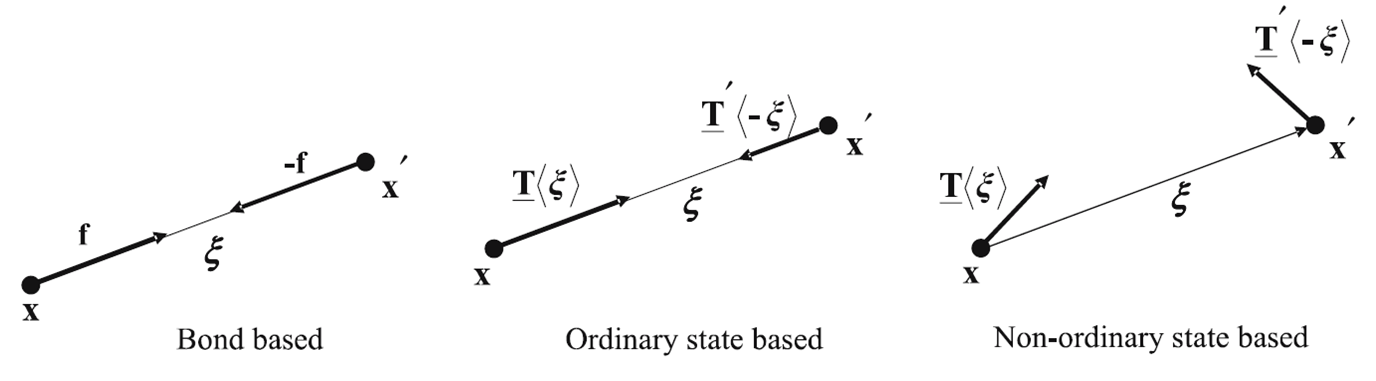
\includegraphics[width=\linewidth]{chap/image/peridynamics_models}

  \caption{\label{peridynamics_models}
           bond-based, ordinary state-based, non-ordinary state-based 模型对比示意图。在 bond-based 模型中,粒子之间彼此施加的力相等,且沿两者直线方向,因此本质上是质点弹簧系统。在 ordinary state-based 模型中,力沿两者直线方向,但彼此施加的力不一定相等。在 non-ordinary 模型中,对力的大小和方向并无约束,但需遵守动量和角动量守恒规律。图片取自\mycite{Silling}{2007}。
          }
\end{figure}

虽然近场动力学理论被倾向于用于处理线性弹性材料,但随着近场动力学理论的不断发展,学术界和工业界越来越意识到其理论优越性,其潜力也被不断挖掘。本文工作和其他实践证明其同样可以适用于处理非线性弹性、塑性、粘滞弹性、粘滞塑性等材料。限于本文篇幅,在此不能对近场动力学进行完整地阐述,更详细的介绍请参见\mycite{Madenci}{2014}。 本文工作所用的近场动力学模型基于 ordinary state-based 模型,但对原有理论进行了重新阐述以及修改,以适应图形学领域应用的特点。

\section{研究成果和创新点}

本文的主要研究成果是提出并实现了一种新的基于近场动力学理论的无网格框架来进行弹塑性物体的形变和碎裂仿真,其能够克服 FEM 在拓扑网格上面存在的困难,避免 remeshing 操作所引发的效率低下和实现复杂问题。在物理动力学上,其能够较为精确地仿真形变和碎裂行为,提供物理上和视觉上可信服的结果。此外,为表达弹塑性碎裂行为的视觉效果,本文还提出一种新的简单可用的嵌网格方法。本工作所提框架易于实现,并具有较强的可扩展性,在效率上相对于传统方法也更具优势。

具体而言,本文的创新点主要在于三点:
\begin{enumerate}
  \item 基于近场动力学理论,提出一种新的基于近场动力学理论无网格仿真框架。其支持包括弹塑性材料的弹性形变、塑性形变、弹塑性碎裂、脆性碎裂等多种复杂物理行为,同时能够很好地解决在 FEM 中不连续性引起的奇异值问题,避免复杂耗时的 remeshing 操作。此外,本文还对模型进行进一步扩展,使其能够支持简单的各向异性行为。
  \item 设计一种简单有效的嵌网格方法,所设计策略能够从几何表示上对物体的形变和碎裂行为进行追踪,能用于后续的碰撞处理以及提供高质量网格以用于渲染。本文力图所提的嵌网格方法是有效,完备的,可应用于其他无网格框架,且具有良好的扩展性。
  \item 基于 Physika\footnote{http://github.com/PhysikaTeam/Physika} 物理引擎,设计并实现相应的模型和主要算法,并对实现进行大量的实验和验证工作,和已有方法(FEM)进行充分对比。
\end{enumerate}

\section{本文组织结构}
本文主要分为六章。

第一章主要是本文工作的研究背景,介绍基于物理的仿真包括形变和碎裂仿真的研究意义以及在各领域的应用需求情况。梳理关于形变仿真、碎裂仿真、近场动力学的相关工作,同时明确本文的研究问题,介绍本文的研究成果和工作的创新点。

第二章概述性地介绍了物理仿真的基本原理,以及碎裂仿真的基本流程。并针对碎裂仿真中的三个主要要素,本构模型、碎裂模型、和离散时间积分在仿真中所扮演角色和作用,进行了一般性地介绍。最后针对近场动力学方法(PDM)的基本特征和本构方程基本形式,以及从经典连续介质力学到近场动力学的模型推导,作了较为详细的阐述。

第三章主要研究基于近场动力学理论的形变体仿真。全章首先重新表述了全文工作所用的弹塑性本构模型,并详细介绍了对应的离散化框架以及嵌网格策略。最后利用全章所述模型和方法,通过多样化材料的材质属性,对不同材料的形变行为进行模拟,展示相应的实验结果,并和 FEM 进行了充分的对比。

第四章主要研究基于近场动力学理论的碎裂仿真。在第三章的基础上,全章首先介绍了全文所用的碎裂模型,并对原有本构模型进行扩展,以支持简单的各向异性的碎裂行为。接着在已有离散框架上,详细介绍了拓扑网格更新方法以显式追踪碎裂带来的物体边界改变。最后展示了基于所述方法所取得的结果,实验证明本文所提方法能够高逼真地仿真弹脆性碎裂以及塑性碎裂。

第五章是对全文的工作总结和展望。



	\chapter{物理仿真和近场动力学方法(PDM)介绍}

\section{物理仿真之基本原理}
绝大多数物理仿真流程遵循相同的基本流程,都可以认作是牛顿第二定律 $F = Ma$ 的不同形式的体现。如图\ref{fig_physically_based_animation} 所示:
\begin{figure}[htbp!]
  \centering
  \captionsetup{justification=centering}
  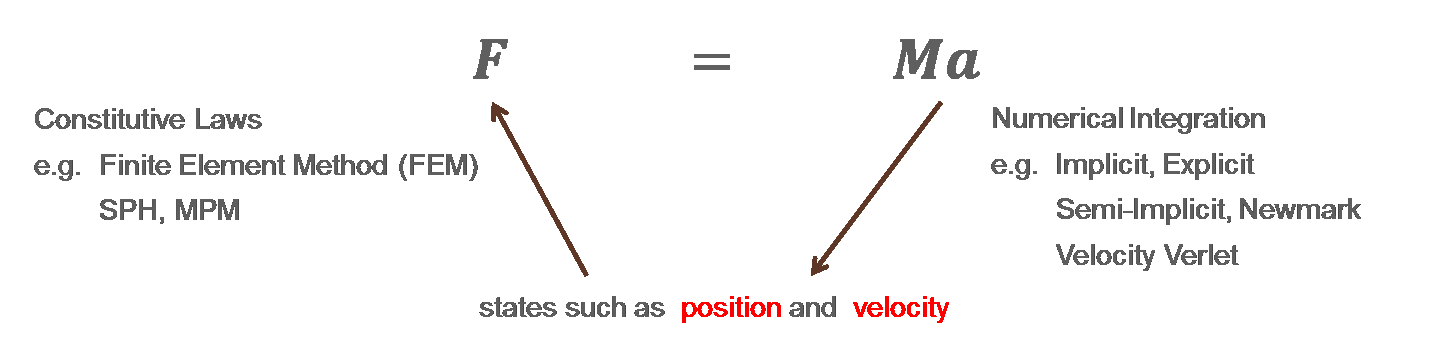
\includegraphics[width=\linewidth]{chap/image/physically_based_animation}

  \caption{\label{fig_physically_based_animation}
           物理仿真动力学循环示意图。物体所受内外力、加速度、以及物体状态构成动力学循环三角。
          }
\end{figure}

在物理仿真中,需要关注三个核心的动力学要素:物体所受内外力,加速度,以及物体的状态。从物体的当前所处状态,即物体的位置和速度信息,来推导物体当前各部分所受力,所涉及的是物理仿真中最为关键的部分——动力学本构模型。通俗而言,本构模型描述的是材料的形变与动力学行为之间的关系,一般也称为内力模型。常见的本构模型包括用来描述固体运动的有限元方法(FEM)、用来描述流体运动的光滑粒子动力学(SPH)\textcolor{blue}{(M\"{u}ller et al. )\parencite{Muller2003}}、 以及适合对雪进行建模的物质点法(MPM)\mycite{Stomakhin}{2013}等。关于本构模型的一般性介绍,将呈现于章节\ref{constitutive_model}。

根据物体所受力 $F$,则可以根据牛顿第二定律直接获得物体的加速度 $a$。 而从物体所受加速度进一步推导得到物体的当前状态,所涉及到的则是离散时间积分算法。离散积分算法的作用是在给定时间步 $\Delta t$ 下,物体的状态将以何种方式进行更新。不同的离散时间积分算法对物理仿真的稳定性、精确性和效率有重大影响,本文将在\ref{numerical_method} 小节详细阐述。

可以看到,物体所受内外力、加速度、以及物体状态构成了一个动力学循环三角,并通过牛顿第二定律、本构模型、数值积分算法进行衔接。绝大部分仿真算法都是采用关键帧(key frame)的形式,因为在复杂场景中,物体的运动几乎不可能以解析的形式来表达,因此需要随着时间步而不断向前迭代,以此获得物体完整的运动状态序列。

\section{碎裂仿真之基本流程}
碎裂仿真是物体仿真的一个具体特化,但相对于传统仿真更具复杂性。其原因不仅在于碎裂模式的多样化,更在于在碎裂发生的情况下,物体本身拓扑表达的变化,导致物体单元体或节点的数量也将发生改变。典型的碎裂仿真流程如图
\ref{fig_fracture_animation_pipeline}总结:
\begin{figure}[htbp!]
  \centering
  \captionsetup{justification=centering}
  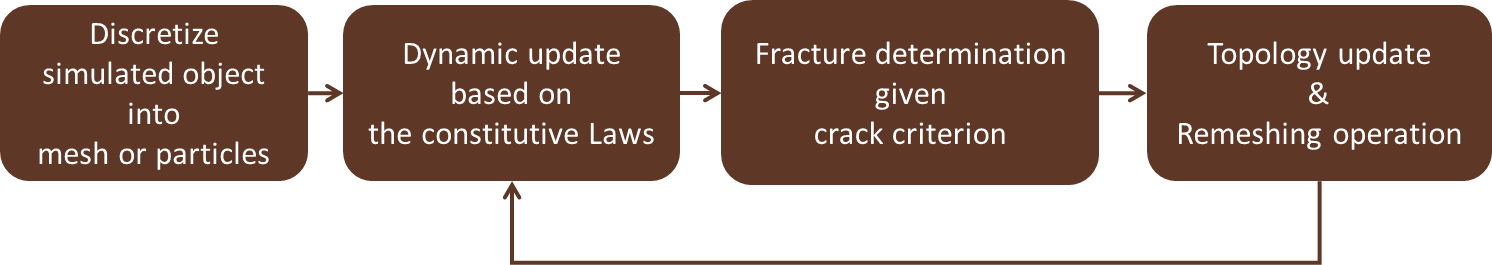
\includegraphics[width=\linewidth]{chap/image/fracture_animation_pipeline}

  \caption{\label{fig_fracture_animation_pipeline}
           碎裂仿真的基本流程。主要分为四个关键步骤,分别是物体离散、动力学更新、碎裂发生判断,拓扑更新。
          }
\end{figure}

从图\ref{fig_fracture_animation_pipeline}可以看出,碎裂仿真主要包含四个步骤。

第一个步骤是在动力学仿真开始前,需要以合适的方式对物体进行离散,由于计算资源是有限的,因此不可能以无限微分的方式来对物体进行建模计算,而只能用有限的状态集表示。一般而言,离散方式和本构模型直接挂钩。对于传统基于网格的方法,如 FEM,通常将物体离散成四面体或六面体体网格,对于薄壳体则离散成三角面片网格\mycite{Pfaff}{2014}。而对于无网格方法,则通过粒子集合来表示物体\mycite{Pauly}{2005}。

第二个步骤是在物体已知状态下,通过动力学本构模型和数值积分算法来对物体的状态进行更新,这一步骤是所有物理仿真所必须的。

第三个步骤和第四个步骤是根据给定的碎裂标准和阈值判断物体中的某些节点是否应该发生碎裂,碎裂模型一般建立在已有的本构模型之上,本文将在\ref{fracture_model}进行一般性介绍。如果判断物体部分节点发生碎裂,则往往需要对拓扑进行更新。对于有网格方法,在必要情况下,还需要对拓扑网格进行 remeshing 操作以对网格进行精化。在拓扑更新完之后,将进入下一个循环的动力学更新。关于本文工作所用的碎裂模型和拓扑更新方式,将分别在第三章和第四章进行阐述。

\section{本构模型泛述}
\label{constitutive_model}
在图形学领域及工程材料领域,一般研究的是物质的宏观运动。但实际上物质都是由大量分子组成的,分子间的真空区尺度远大于分子本身,并且每个分子在无休止的做不规则运动,相互间经常碰撞,交换着动量和能量。因此物质的微观结构和运动无论在时间上还是空间上都充满着不均匀性、离散性和随机性。而另一方面人们用仪器测量或者用肉眼观察到的物质宏观结构和运动却又明显呈现出均匀性、连续性和确定性。这两种特性如此之不同却又和谐统一地表现于物质之中。研究物体的宏观运动存在两种不同的途径,一种是基于统计物理的方法,其直接从分子和原子的运动出发,采用统计平均的方法建立宏观物理量满足的方程,但这种方法迄今为止还不完善。另一种方法则是以连续介质为假设,认为物质连续地充满物体所在的整个空间,构成物体的物质单元或质点在微观上认为充分大,但在宏观上又被认为足够小。其具有的宏观物理量(质量、速度、力)满足一切都应遵循的物理定律及物理性质,例如牛顿定律、质量守恒定律和能量守恒定律等。这一假设已经被学术界广为采用,并且在揭示物质材料的动力学性质上已经取得巨大成功。

现有的本构模型几乎都基于连续介质假设,典型如描述固体的连续介质力学\mycite{Eduardo}{2013}和描述流体的Navier-Stokes方程。本构模型描述的是在连续介质假设下,物体某微元根据自身状态以及周围状态所作出的反应,其一般以解析形式表达在外力和边界条件作用下,物体产生的形变行为将如何反抗相应的作用力。

本文工作所采用的近场动力学理论和连续介质力学中的线性模型在理论上是对等的,所以下面对连续介质力学的理论基础尤其是线性模型做必要介绍。

在连续介质力学中,用来表示物体形变的关键变量是 $\F \in \textbf{R}^{3\times3}$,其定义为

\begin{equation}
\F \equiv \frac{\partial(\boldmath{x}, \boldmath{y}, \boldmath{z})}{\partial(\X, \Y, \Z)}
=
\left(
  \begin{array}{ccc}
    \frac{\partial\boldmath{x}}{\X}& \frac{\partial\boldmath{x}}{\Y} & \frac{\partial\boldmath{x}}{\Z} \\
    \frac{\partial\boldmath{y}}{\X}& \frac{\partial\boldmath{y}}{\Y} & \frac{\partial\boldmath{y}}{\Z} \\
    \frac{\partial\boldmath{z}}{\X}& \frac{\partial\boldmath{z}}{\Y} & \frac{\partial\boldmath{z}}{\Z} \\
  \end{array}
\right)
\end{equation}

其中$\X, \Y, \Z$表示的是形变之前的位置,亦即参考/未形变空间(reference/undeformed space)的位置。$\boldmath{x}, \boldmath{y}, \boldmath{z}$ 则表示形变后的位置,亦即在世界空间(world space)的位置。在形变梯度的基础上,可以进一步定义格林应变张量 $\E \in \textbf{R}^{3\times3}$(Green strain tensor),即

\begin{equation}
\E = \frac{1}{2}\left(\F^{T}\F - \textbf{I}\right)
\end{equation}

不难看出,格林应变张量是关于形变的二次函数,也即其在几何上是非线性的,并且具有旋转不变性。使用格林应变张量的模型(e.g. Stvk Model)在求解上将更为复杂,可以对其进行线性近似(linear approximation),得到柯西应变张量(Cauchy strain tensor)

\begin{equation}
\mathbf{\epsilon} = \frac{1}{2}(\F^T + \F) - \textbf{I}
\end{equation}

柯西应变张量是关于形变的线性函数,在求解上也较为简便。但其并不具有旋转不变性,也即当只发生刚体的旋转时,将会产生实际上并不应该存在的力(ghost force)。为克服此一问题,更多的是采用共旋线性模型(Corotated Linear Model),其基本原理是对形变梯度 $\F$ 进行极化分解(polar decomposition),去除其旋转分量。

\begin{equation}
\begin{aligned}
\F & = \textbf{RS} \\
\mathbf{\epsilon}_c & = \textbf{S} - \textbf{I}
\end{aligned}
\end{equation}

上述公式中 $\textbf{R}$ 表示旋转部分,$\textbf{S}$ 则为形变部分,其是对称张量。在形变张量 $\mathbf{\epsilon}$的定义中,可以看到旋转部分 $\textbf{R}$ 被舍弃,而只与形变相关,因此共旋线性模型具有旋转不变性。本文工作所用本构模型将基于全新的近场动力学理论,其是连续介质力学中的线性模型推导而来,并且同样具有旋转不变性,本文将在第三章进行详细阐述。

虽然几何上对于形变的度量具有线性和非线性,但在材质模型上,大多数工作都是采用线性模型来计算能量密度 $\mathbf{\psi} $,应力张量$\mathbf{\sigma}$,具体如下:

\begin{equation}
\begin{aligned}
\mathbf{\Psi} = &\frac{1}{2}\mathbf{\epsilon}^T\textbf{C}\mathbf{\epsilon}\\
\mathbf{\sigma} = &\textbf{C}\mathbf{\epsilon}
\end{aligned}
\end{equation}

其中考虑形变张量$\mathbf{\epsilon}$和应力张量$\mathbf{\sigma} $的对称性,将其重整为向量形式,

\begin{equation}
\begin{aligned}
\mathbf{\epsilon} &= \left(
                      \begin{array}{ccccccc}
                         \mathbf{\epsilon}_{xx}\quad
                         \mathbf{\epsilon}_{yy}\quad
                         \mathbf{\epsilon}_{zz}\quad
                         \mathbf{\epsilon}_{yz}\quad
                         \mathbf{\epsilon}_{xz}\quad
                         \mathbf{\epsilon}_{xy}
                      \end{array}
                    \right)^T\\
\mathbf{\sigma} &= \left(
                      \begin{array}{cccccc}
                         \mathbf{\sigma}_{xx}\quad
                         \mathbf{\sigma}_{yy}\quad
                         \mathbf{\sigma}_{zz}\quad
                         \mathbf{\sigma}_{yz}\quad
                         \mathbf{\sigma}_{xz}\quad
                         \mathbf{\sigma}_{xy}
                      \end{array}
                  \right)^T
\end{aligned}
\end{equation}

最后,$\textbf{C}$ 被称为物质材质矩阵(material property matrix),定义为

\begin{equation}
\textbf{C} = \left(
               \begin{array}{cccccc}
                 \kappa + (4\mu/3) & \kappa - (2\mu/3) & \kappa - (2\mu/3) & 0 & 0 & 0 \\
                 \kappa - (2\mu/3) & \kappa + (4\mu/3) & \kappa - (2\mu/3) & 0 & 0 & 0 \\
                 \kappa - (2\mu/3) & \kappa - (2\mu/3) & \kappa + (4\mu/3) & 0 & 0 & 0 \\
                 0 & 0 & 0 & \mu & 0 & 0 \\
                 0 & 0 & 0 & 0 & \mu & 0 \\
                 0 & 0 & 0 & 0 & 0 & \mu \\
               \end{array}
             \right)
\end{equation}
上式中$\kappa$ 和 $\mu$ 分别表示体积模量和剪切模量。

在给定离散框架下(如 FEM),则可以相应计算形变梯度 $\textbf{F}$,进而获得应力张量 $\mathbf{\sigma}$,最终可以通过加权平均的方式算得作用力,并施加到离散模型的各个节点之上。

\section{碎裂模型泛述}
\label{fracture_model}

碎裂本质上是材料一种结构屈服和能量释放行为,在物理仿真中通过专门的碎裂模型来描述。碎裂模型通常直接建立在本构模型之上,其主要功能在于两点。第一,判断碎裂是否发生。第二,判断裂纹生长的方向。碎裂模型一般是通过在基于本构模型进行相应计算时,通过已得的物理量构建一个衡量碎裂的中间标准物理量,以及计算碎裂是否发生以及碎裂方向。

\begin{figure}[!htb]
  \centering
  \captionsetup{justification=centering}
  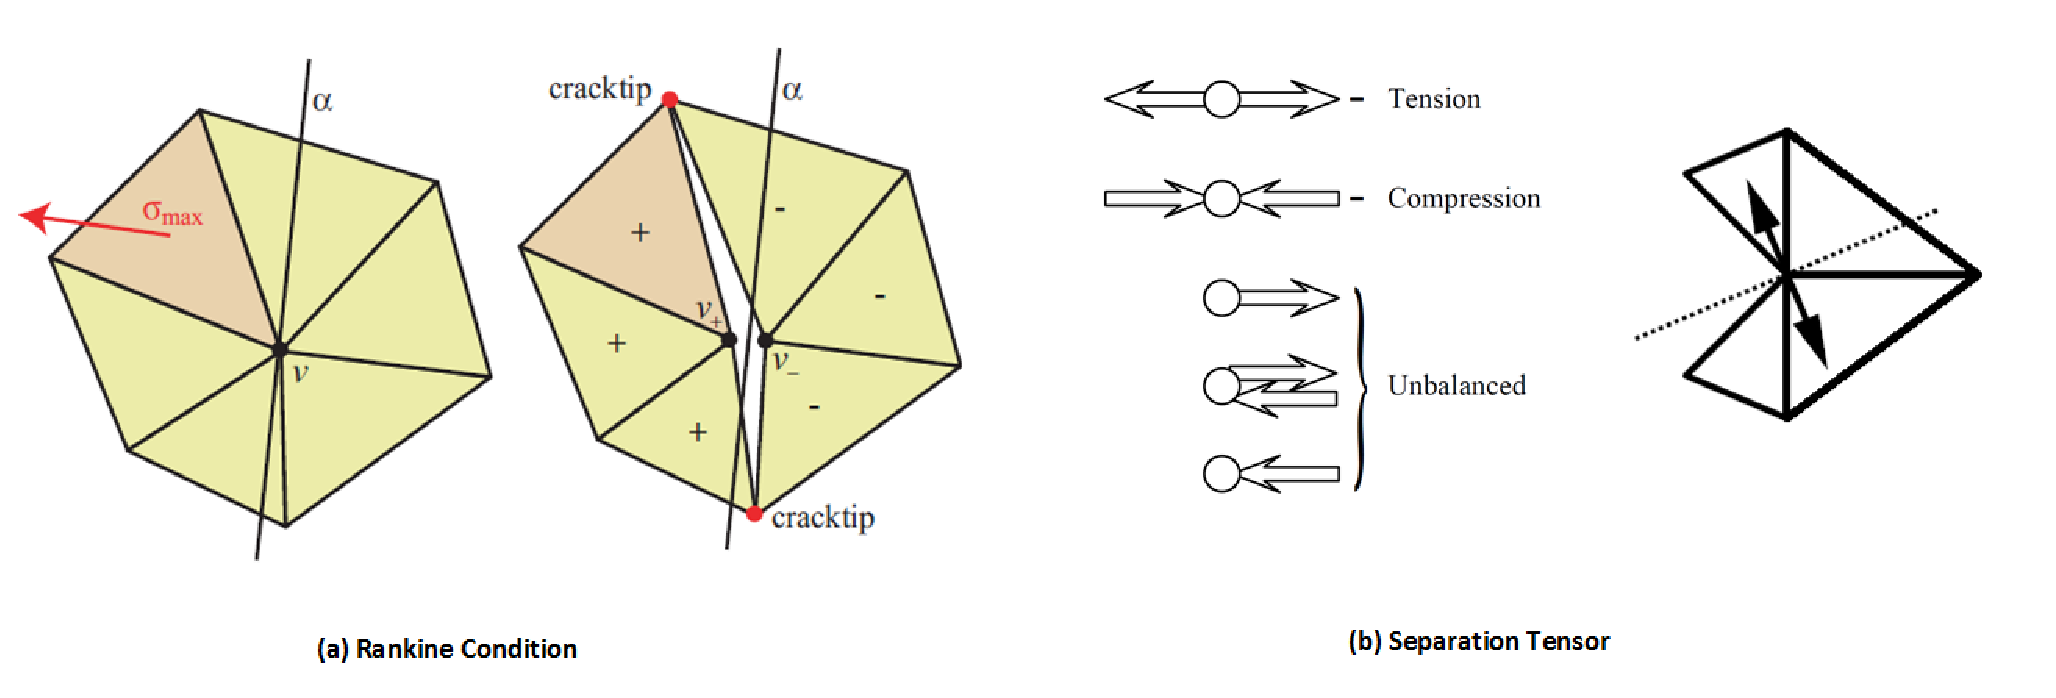
\includegraphics[width=\linewidth]{chap/image/fracture_model}

  \caption{\label{fracture_model}
           碎裂模型示意图。左边为Rankine Condition,右边为 Separation Tensor。图片分别取自\textcolor{blue}{(M\"{u}ller et al. )\parencite{Muller2004}} 和\textcolor{blue}{(O'Brien et al. )\parencite{OBrien1999}}。
          }
\end{figure}

最常用的碎裂模型包括 Rankine Condition,其基本原理是计算物质节点的主应力大小$\mathbf{\sigma}_{max}$ 以及主应力方向 $\textbf{n}_{max}$,如果$\mathbf{\sigma}_{max}$ 超出阈值则认定碎裂发生,并且裂纹方向即为$\textbf{n}_{max}$。 应用此碎裂模型的典型工作包括\textcolor{blue}{(M\"{u}ller et al.)\parencite{Muller2004}}。 但Rankine Condition 的缺陷是即使某一方向受力较大,也会导致碎裂发生,而事实上碎裂是由相互抵消的力(挤压或者撕扯)的大小而决定的。因此,另一种常用的碎裂模型是 Separation Tensor\textcolor{blue}{(O'Brien et al.)\parencite{OBrien1999}} ,其计算的是相互抵消的力最大的方向和应力大小,因此克服Rankine Condition的缺陷,不过其在计算上相对要较为复杂。两种碎裂模型的示意图如图\ref{fracture_model}所示。

对于质点弹簧系统或者无网格中的方法,其拓扑关系通过粒子与粒子之间的连接而决定的。因此,在碎裂模型上往往不涉及裂纹生长的方向,而是可以直接通过去除粒子之间的相互作用力来体现。在无网格框架中,最常用的碎裂模型是临界伸长量(critical stretch)。假设粒子之间通过弹簧相连,如果其伸长比例超过阈值,则断裂发生。本文所用的碎裂模型类似于 critical stretch,但对其有所改进,具体在第三章详述。

\section{离散时间积分}
\label{numerical_method}
在章节\ref{related_work}所阐述的有网格方法和无网格方法本质上是在空间上对物体进行离散化,而求解物体的运动还需要在时间维度上进行离散化,在时间维度上的离散化数值积分被称为离散时间积分。精确性(accuracy)和稳定性(stability)是衡量离散时间积分算法优劣的两大指标,其中精确性衡量的是离散积分的解与连续解之间的误差,而稳定性衡量的是误差是否会随时间累积。关于数值积分的详细介绍,参见\mycite{Michael}{1997}。

离散时间积分决定以何种方式来对系统中的状态进行更新。在大多数系统中,通常需要关心的状态更新是位置 $\textbf{x}$ 和速度 $\textbf{v}$。 对于无网格方法,$\textbf{x}$ 和 $\textbf{v}$ 被直接赋予到粒子之上。而对于有网格方法,虽然整体的物理动力学计算是基于网格中的单元体的,但实际上单元体在拓扑上仍然由节点连接而成,最后的计算结果仍然将会以加权平均的方式施加到各个顶点。

假设某粒子 $i$ 所受内力为 $\fin$,所受外力为$\fex$,速度为$\vi$,位置为$\xii$,质量为 $m_i$。则根据速度的定义以及牛顿第二定律,得到:
\begin{equation}
\label{eq1}
\left\{ \begin{array}{l}
\frac{\textrm{d}\xii}{\textrm{d}t} = \dot{\xii}=\vi\\
\frac{\textrm{d}\dot{\xii}}{\textrm{d}t} = \frac{\textrm{d}\vi}{\textrm{d}t}=\frac{\fin + \fex}{m_i}
\end{array} \right.
\end{equation}
注意在上述公式中$\xii$和$\vi$都是关于时间的函数,离散时间积分是通过$\xii(t_0)$和$\vi(t_0)$来求解$\xii(t_0 + \Delta t)$ 和$\vi(t_0 + \Delta t)$的状态。

最常见的两种时间积分算法分别是显式欧拉积分(explicit Euler integration)和隐式欧拉积分(implicit Euler integration)。在下面小节中,我们将分别进行介绍。

\subsection{显式欧拉积分}
\label{explicit_euler_method}

\begin{figure}[!htb]
  \centering
  \captionsetup{justification=centering}
  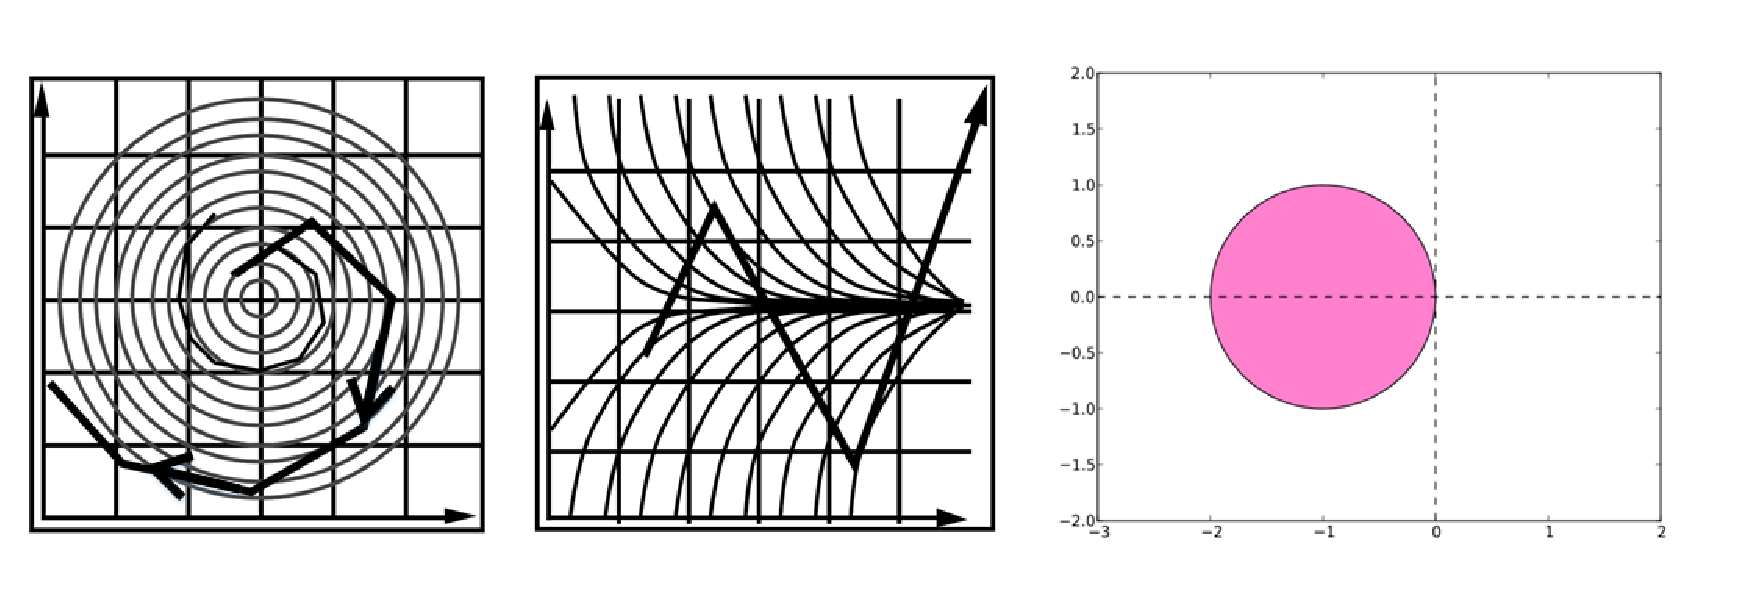
\includegraphics[width=\linewidth]{chap/image/explicit_method}

  \caption{\label{explicit_method}
           显示欧拉积分。随着仿真的进行,误差将很容易累积,从而导致仿真系统崩溃。粉色区域为绝对稳定区域。图片取自\mycite{Witkin}{1997}
          }
\end{figure}

显式积分亦称前向欧拉积分(forward Euler method),其思想来源于在 $t_0$ 时刻的一阶泰勒展开 $f(t_0 + \Delta t) \approx f(t_0) + \dot{f}(t_0)\Delta t$,$t_0 + \Delta t$ 时刻的状态完全直接由 $t_0$ 时刻的状态决定。具体而言,
\begin{equation}
\left\{ \begin{array}{l}
\vi(t_0+\Delta t) = \vi(t_0)+\frac{\fin(t_0) + \fex(t_0)}{m_i}\Delta t\\
\xii(t_0+\Delta t) = \xii(t_0)+\vi(t_0)\Delta t
\end{array} \right.
\end{equation}

显式欧拉积分是最容易实现的离散积分方式,并且可以直接并行化。在数值准确性上其具备一阶数值精度,但稳定性较差。当时间步长 $\Delta t$ 较长时,容易累积误差而致使整个仿真系统崩溃,如图\ref{explicit_method}。因此使用显式积分的仿真系统往往需要设置较小的时间步,并且同时添加阻尼力保证仿真的稳定性。可以进行些许修改从而一定程度上改善其稳定性:
\begin{equation}
\left\{ \begin{array}{l}
\vi(t_0+\Delta t) = \vi(t_0)+\frac{\fin(t_0) + \fex(t_0)}{m_i}\Delta t\\
\xii(t_0+\Delta t) = \xii(t_0)+\vi(t_0 \textcolor{red}{ + \Delta t})\Delta t
\end{array} \right.
\end{equation}
这种形式的数值积分算法被称为半隐式欧拉积分(Semi-implicit Euler integration)。本文工作大部分都采用此种形式的积分算法,具体计算流程可用如下伪码表示:\\

\noindent\fbox{
\parbox{0.6\textwidth}{

//initialization\\
(1) \textbf{forall} particles $i$ \\
(2) \qquad initialize $m_i$ and other necessary info\\
(3) \qquad $\xii \leftarrow \xii(t_0)$\\
(4) \qquad $\vi \leftarrow \vi(t_0)$\\
(5) \textbf{endfor}\\\\
//simulation loop\\
(6) \textbf{loop}\\
(7) \qquad \textbf{forall} particles $i$\\
(8) \qquad \qquad calculate $\fin$ from constitutive laws\\
(8) \qquad \qquad calculate $\fex$ from boundary conditions\\
(9) \qquad \qquad $\vi\leftarrow \vi + \Delta t\cdot \frac{\fin + \fex}{m_i}$\\
(10) \qquad\qquad $\xii\leftarrow \xii +\Delta t\cdot \vi$\\
(11) \qquad\textbf{endfor}\\
(12) \qquad display the system every $n^{th}$ time\\
(13) \textbf{endloop}
}
}\\

\subsection{隐式欧拉积分}
\label{implicit_euler_method}

\begin{figure}[!htb]
  \centering
  \captionsetup{justification=centering}
  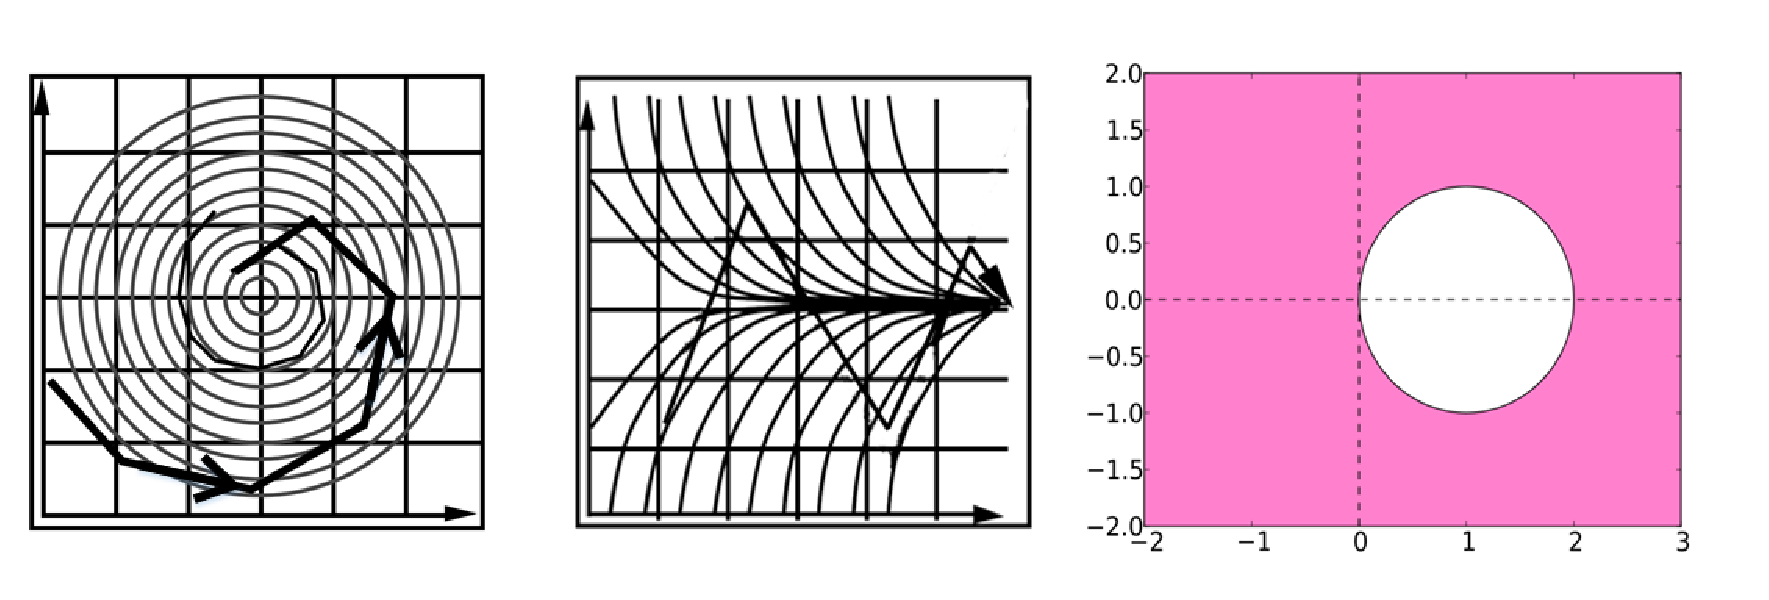
\includegraphics[width=\linewidth]{chap/image/implicit_method}

  \caption{\label{implicit_method}
           隐式欧拉积分。隐式欧拉积分理论上可认为是无条件稳定的,并且自带阻尼效果。图中粉色区域所示为绝对稳定区域。
          }
\end{figure}

不同于显式欧拉积分,隐式欧拉积分理论上可认为是绝对稳定的,其误差并不随时间而积累。一般认为隐式欧拉积分方法自带阻尼效果,其会导致能量的耗散,如图\ref{implicit_method}所示。隐式欧拉积分的思想来源于在 $t_0 + \Delta t$ 时刻的一阶泰勒近似$f(t_0) \approx f(t_0 + \Delta t) - \dot{f}(t_0 + \Delta t)\Delta t$,因此也称之为向后欧拉算法(backward Euler method)。其具体积分形式可写为:
\begin{equation}
\left\{ \begin{array}{l}
\vi(t_0+\Delta t) = \vi(t_0)+\frac{\fin(t_0 \textcolor{red}{+ \Delta t}) + \fex(t_0 \textcolor{red}
                                  {+ \Delta t})}{m_i}\Delta t\\
\xii(t_0+\Delta t) = \xii(t_0)+\vi(t_0 \textcolor{red}{ + \Delta t})\Delta t
\end{array} \right.
\end{equation}

进一步,
\begin{equation}
\label{eqa25}
\left\{ \begin{array}{l}
\Delta \vi = \frac{\fin(t_0 \textcolor{red}{+ \Delta t}) + \fex(t_0 \textcolor{red}
                                  {+ \Delta t})}{m_i}\Delta t\\
\Delta \xii = \left(\vi(t_0) + \Delta \vi\right)\Delta t
\end{array} \right.
\end{equation}

其中 $\Delta \vi = \vi(t_0 + \Delta t) - \vi(t_0)$ 表示速度增量, $\Delta \xii = \xii(t_0 + \Delta t) - \xii(t_0)$ 表示位置增量,$\fin(t_0 \textcolor{red}{+ \Delta t})$ 和 $\fex(t_0 \textcolor{red}{+ \Delta t})$ 分别代表在 $t_0 + \Delta t$ 时刻的内力和外力。一般而言,$\fex(t_0 \textcolor{red}{+ \Delta t})$ 可以直接用 $\fex(t_0)$ 近似,然而$\fin(t_0 \textcolor{red}{+ \Delta t})$则不然。事实上,除非 $\fin(t_0 \textcolor{red}{+ \Delta t})$ 是线性函数,亦即所仿真材料是线性材料,否则在求解时其并非已知。因此如果$\fin(t_0 \textcolor{red}{+ \Delta t})$ 是非线性函数(即非线性材料),则此时是无法对其进行精确求解的,只能对其进行一阶泰勒近似,亦即
\begin{equation}
\fin(\xii(t_0) + \Delta \xii(t_0),\vi(t_0)+\Delta \vi) = \fin(t_0) +
                                                         \sum\frac{\partial \fin(t_0)}{\partial \xj}\Delta \xj+
                                                         \sum\frac{\partial \fin(t_0)}{\partial \vj}\Delta \vj
\end{equation}

注意在 $t_0 + \Delta t$ 时刻,$\fin$ 是关于$\xii(t_0 + \Delta t)$ 和 $\vi(t_0 + \Delta t)$的函数,通常 $\fin$ 并不和速度相关,所以上式可以进一步简化为

\begin{equation}
\label{eqa27}
\fin(t_0)+ \Delta t) = \fin(t_0) +\sum\frac{\partial \fin(t_0)}{\partial \xj}\Delta \xj
\end{equation}

将式\ref{eqa27}代入\ref{eqa25},并消去 $\Delta \xii$,则可得

\begin{equation}
\Delta \vi = \frac{\Delta t}{m_i}\left[\fin(t_0) + \fex(t_0)\right]
           + \sum\frac{\Delta t^2}{m_i} \frac{\partial \fin(t_0)}{\partial \xj}
             \left(\vj(t_0) + \Delta \vj\right)
\end{equation}

可以看出,上述公式左边是关于粒子 $i$ 的速度增量$\Delta \vi$,而右边则和周围粒子$j$的速度增量 $\Delta \vj$相关,这是由本构模型决定的。所以不同于显式方法,隐式积分方法是没有办法对状态进行单独求解的,而只能进行全局求解。我们需要将其扩充为向量形式,如下

\begin{equation}
\Delta \textbf{v} = M^{-1}\Delta t\left[\textbf{f}^{int}(t_0) + \textbf{f}^{ext}(t_0)\right]
                  + M^{-1}\Delta t^2 \frac{\partial \textbf{f}^{int}(t_0)}{\partial \textbf{x}}
                    \left(\textbf{v}(t_0) + \Delta\textbf{v}\right)
\end{equation}

其中$M$为质量对角矩阵。将上述方程进行重整,可以得到最终形式:

\begin{equation}
\left(\hat{I} - M^{-1}\Delta t^2 \frac{\partial \textbf{f}^{int}(t_0)}{\partial \textbf{x}}\right)\Delta \textbf{v} = M^{-1}\Delta t\left[\textbf{f}^{int}(t_0) + \textbf{f}^{ext}(t_0)\right]
                  + M^{-1}\Delta t^2 \frac{\partial \textbf{f}^{int}(t_0)}{\partial \textbf{x}}\textbf{v}(t_0)
\end{equation}

或

\begin{equation}
\left(M - \Delta t^2 \frac{\partial \textbf{f}^{int}(t_0)}{\partial \textbf{x}}\right)\textbf{v}(t_0 + \Delta t) = \Delta t\left[\textbf{f}^{int}(t_0) + \textbf{f}^{ext}(t_0)\right]
                  + M\textbf{v}(t_0)
\end{equation}

其中 $\textbf{K} = \frac{\partial \textbf{f}^{int}(t_0)}{\partial \textbf{x}}$ 被定义为刚度矩阵(stiffness matrix)。不难看出,在隐式积分算法下,问题最终转化为一个线性系统$\textbf{Ax} = \textbf{b}$问题的求解。对于大规模的线性矩阵求解问题,一般采用迭代法进行求解,如 Jacobi 迭代法或者 Gauss-Seidel 迭代法。其中 Jacobi 迭代法收敛速度较慢,但适于并行,Gauss-Seidel 迭代法则相反。此外,考虑刚度矩阵 $\textbf{K}$ 一般具有对称性,更多的是采用预置共轭梯度的办法来进行求解(PCG),其具有非常良好的收敛速度。在具体实现时,刚度矩阵 $\textbf{K}$ 往往不需要显式构造,只需要提供计算 $\textbf{K} \cdot \Delta \textbf{x}$ 的接口,进一步减少存储空间和提高效率。

隐式欧拉积分在 FEM 和其他无网格方法应用都较为普遍,其相对于显式积分方法在稳定性上具有明显优势。虽然隐式方法实现更为复杂,但由于能够对时间步 $\Delta t$的限制有所放松,所以最终仿真效率能够领先于显式积分方法。不过由于近场动力学本身的特殊性,其在计算刚度矩阵时$\textbf{K}$相对于一般系统要多出一层复杂度,所以在本工作中,我们只针对规模较小系统尝试隐式欧拉积分,具体原因将在第三章进行说明。


\section{近场动力学方法(PDM)简介}

\subsection{基本特征和形式}
\label{pdm_basic_feature}
在上节中已经提及,相对于其他动力学模型,近场动力学的两大基本特点分别是非局域性以及积分形式的表述。

关于粒子之间作用的局域性问题,存在两种截然不同的理论。以经典连续介质力学为代表的局域性理论,认为粒子在微观上只和其直接邻域发生作用,而和其他粒子无关。这一假设在很大程度上对材质进行了简化,却又基本上描述了材料的动力学行为,因而在工程领域以及图形学领域应用极多。局域性理论的另一个极端则是分子动力学,其认为每一个粒子和其他粒子都能彼此发生作用,而不仅限于其直接邻居。分子动力学在基础物理领域的仿真应用较大,但在倾向于研究宏观运动行为的图形学领域则应用较少。从局域性的观点来看,近场动力学恰好位于两种理论之间,其假定材质中的物质点会和有限半径范围内的邻域发生作用,因此可认作是连接两种理论的桥梁。如图\ref{peridynamics_comparison}所示:

\begin{figure}[htbp!]
  \centering
  \captionsetup{justification=centering}
  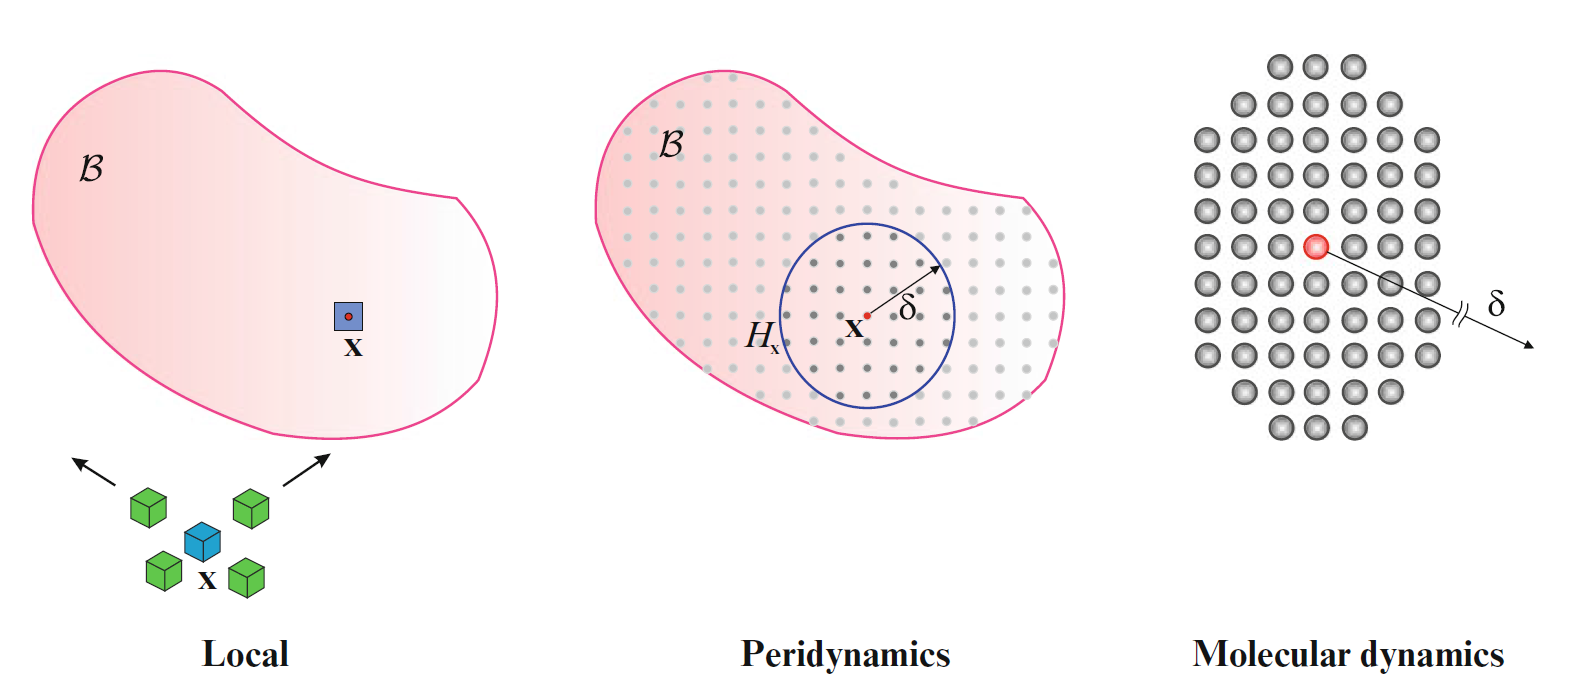
\includegraphics[width=\linewidth]{chap/image/peridynamics_comparison}

  \caption{\label{peridynamics_comparison}
           不同动力学模型的作用域大小对比。左边为局域性理论,粒子只和直接邻域发生相互作用。右边为分子动力学理论,可认定作用半径无限大。而近场动力学位于两者之间,受邻域半径 $\delta$ 范围内的粒子影响。
          }
\end{figure}

对于近场动力学模型,可以根据图\ref{peridynamics_comparison}中图作更为细致的形式化表述。具体而言,材质中的任何一个物质粒子 $\mathbf{x}$ 将会和其周边半径为 $\delta$ 内的粒子发生相互作用,这一半径 $\delta$ 被定义为\textbf{邻域半径}(horizon),而位于邻域半径 $\delta$ 之内的粒子被定义\textbf{邻域}(family),$H_\mathbf{x}$。对于连续性的材料,在离散化之前,邻域范围内的粒子数量可认定是无穷的。从用粒子来表示物体的观点来看,近场动力学的基本思想和其他无网格方法\textcolor{blue}{(M\"{u}ller et al.)\parencite{Muller2003}\parencite{Muller2003}}并无大差异,最大的区别在作用半径 $\delta$ 的定义,这也是近场动力学理论被认定为非局域性理论的原来。 \mycite{Silling}{2003}证明,当 $\delta$ 趋向于0 时,近场动力学模型将会退化为经典的连续介质力学。而当 $\delta$ 区域无穷大时,则会成为连续形式的分子动力学理论。

在近场动力学之前,几乎所有的动力学模型都采用的是微分形式的本构方程(governing function)。最为典型的就是在连续介质力学理论中,本构方程一般使用如下形式,

\begin{equation}
\label{fem_governing_function}
\rho\ddot{\mathbf{u}}(\mathbf{x}) = \nabla\cdot\delta(\mathbf{x})+\mathbf{b}(\mathbf{x})
\end{equation}

其中$\rho$表示粒子的质量密度。$\ddot{\mathbf{u}}$为向量,表示粒子的位移。$\mathbf{b}$表示粒子所受外力,一般包括重力或者由碰撞导致的外力等。类似的符号表示将同样应用于后续近场动力学的本构方程,后面将不再赘述。在方程\ref{fem_governing_function}中,另一个最为关键的物理量是$\nabla\cdot\delta$,即是二阶应力张量$\delta$的散度微分,表示单位体积物理所受的力(力密度)。如前面章节\ref{constitutive_model} 所述, $\delta$的计算尤为关键,其包含物体所有的本构信息。需要尤其注意的是,$\nabla\cdot\delta$ 是关于空间位置的偏微分,而空间微分在不连续之处并不能很好定义,在物体边界以及碎裂发生之处,空间微分很容易导致奇异值问题。因此在基于连续介质力学的离散框架(FEM)以及相关工作中,往往需要额外的工作来特殊对待碎裂问题,例如textcolor{blue}{(O'Brien et al. 1999)\parencite{OBrien1999}},\textcolor{blue}{(O'Brien et al. 2002)\parencite{OBrien2002}}中的 remeshing 操作。事实上,这一问题并不仅仅存在于有网格方法,\mycite{Madenci}{2014}指出,几乎所有的无网格方法使用的都是微分形式的本构方程,因而都不能避免此问题。

不同于以往方法,近场动力学使用的是积分形式的动力学表述,这也是其另一大特征。由于是积分形式,近场动力学的本构方程在不连续处将仍然保持良好定义,并且材质的损伤本身就是模型的一部分。这一优势使得近场动力学非常适合处理不连续问题,尤为是碎裂现象。具体而言,近场动力学中关于物质粒子 $\mathbf{x}$的本构方程可以写为

\begin{equation}
\rho\ddot{\mathbf{u}}(\mathbf{x}) = \int_{H_\mathbf{x}}[\mathbf{T}\langle\mathbf{x}',\mathbf{x}\rangle - \mathbf{T}\langle\mathbf{x},\mathbf{x}'\rangle]dH+\mathbf{b}(\mathbf{x}),
\label{pdm_governing_function}
\end{equation}

其中$\rho, \mathbf{u}, \mathbf{b}$ 的含义同\ref{fem_governing_function}一致。$\mathbf{x}'$ 表示属于 $\mathbf{x}$ 的邻域 $H_\mathbf{x}$ 另外一个物质粒子。$\mathbf{T}\langle\mathbf{x}',\mathbf{x}\rangle$ 和 $\mathbf{T}\langle\mathbf{x},\mathbf{x}'\rangle$ 是两个关键变量,其包含了材质的本构信息。$\mathbf{T}\langle\mathbf{x}',\mathbf{x}\rangle$ 表示粒子 $\mathbf{x}'$ 施加给粒子 $\mathbf{x}$ 的内力,而$\mathbf{T}\langle\mathbf{x},\mathbf{x}'\rangle$ 则相反,表示粒子 $\mathbf{x}$ 施加给粒子 $\mathbf{x}'$ 的内力。注意如章节\ref{pdm_history}所述,这两个变量并不一定相同,但必须同时出现在本构方程中以遵循牛顿第三定律,这一策略类似于 SPH 方法\textcolor{blue}{(M\"{u}ller et al. 2003)\parencite{Muller2003}}。尖括号$\langle\cdot\rangle$ 符号表示关于 $H_\mathbf{x}$的函数,其在\mycite{Silling}{2007}中被定义为\textbf{状态}(state)。需要尤其注意的是本构方程中的积分符号 $\int_{H_\mathbf{x}}$,这是近场动力学模型区别其他理论最根本上的不同。可以看出,整个方程是基于粒子的位移$\mathbf{u}$,而不是基于位移的空间微分的,因此也使得对于不连续问题的处理更加方便以及稳定。在粒子离散框架下,关于邻域 $H_\mathbf{x}$ 的连续积分可以进一步用粒子的累加和来表示,即,

\begin{equation}
\rho\ddot{\mathbf{u}}(\mathbf{x}) = \sum_{\mathbf{x}'\in H_\mathbf{x}}[\mathbf{T}\langle\mathbf{x}',\mathbf{x}\rangle - \mathbf{T}\langle\mathbf{x},\mathbf{x}'\rangle]V_{\mathbf{x}'}+\mathbf{b}(\mathbf{x}),
\label{pdm_governing_function_discrete}
\end{equation}
其中 $V_{\mathbf{x}'}$ 表示粒子 $\mathbf{x}'$ 的体积,其值取决于粒子的分布。

\subsection{模型推导}
\label{pdm_derivation}

在章节\ref{pdm_basic_feature}中,公式\ref{pdm_governing_function_discrete}描述了近场动力学的基本形式和本构方程。但更为关键的是两个重要变量$\mathbf{T}\langle\mathbf{x}',\mathbf{x}\rangle$ 和 $\mathbf{T}\langle\mathbf{x},\mathbf{x}'\rangle$,其蕴含了材质的本构信息,需要以更为形式化的方式来进行表述。$\mathbf{T}\langle\cdot\rangle$ 的具体形式需要通过发掘材质属性,以及物理规律推导来获得,较为合理的方式便是建立在已有的经典连续介质力学基础之上,然后将两个理论进行等效。但由于连续介质力学是局域性的理论,因此我们首先需要对近场动力学作局域性假设。

\subsubsection{局域性假设}
在极限情况下,亦即当$\delta$ 趋于0时,可认为物质粒子 $\mathbf{x}$ 仅和其直接邻居发生相互作用。如图所示,标记为 $k$ 的粒子只和周围六个粒子 $(k-l)$,$(k+l)$,$(k-m)$,$(k+m)$,$(k-n)$,和$(k+n)$ 存在力作用。这和经典连续介质力学一致,参见\mycite{Bonet}{2008}。

\begin{figure}[htbp!]
  \centering
  \captionsetup{justification=centering}
  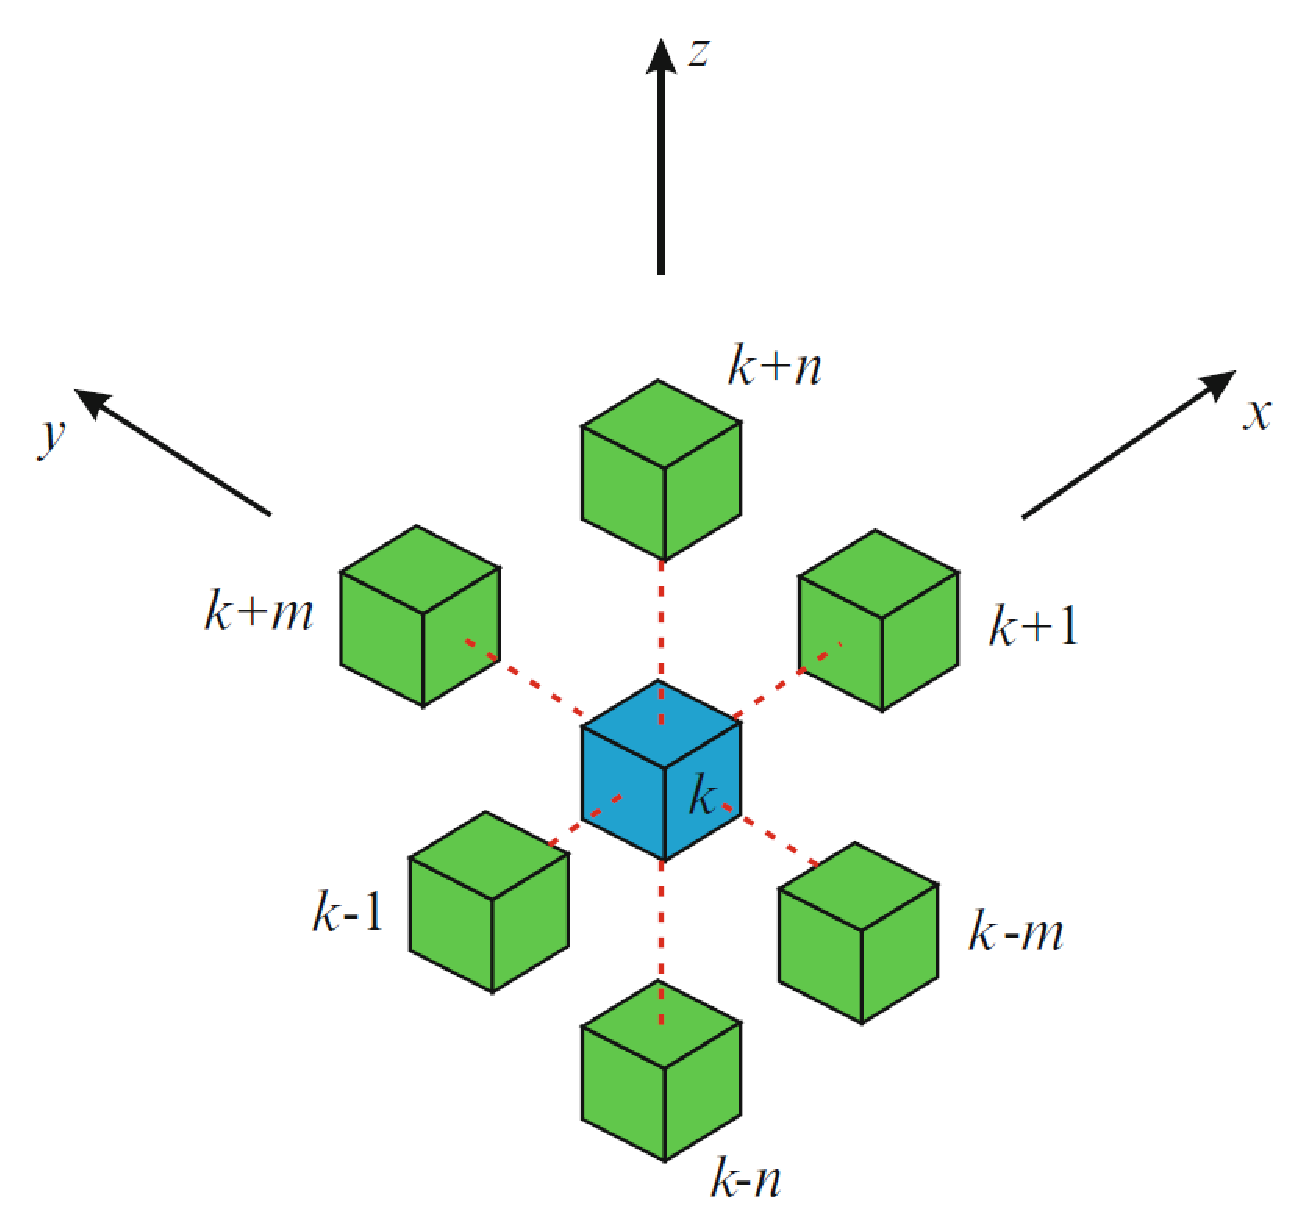
\includegraphics[width=0.5\linewidth]{chap/image/pdm_local}

  \caption{\label{pdm_local}
           局域性假设下的近场动力学。物质粒子 $\mathbf{x}$ 仅仅和$(k-l)$,$(k+l)$,$(k-m)$,$(k+m)$,$(k-n)$,和 $(k+n)$ 周围六个粒子相互作用。图片取自\mycite{Madenci}{2014}。
          }
\end{figure}

在局域性假设下,针对粒子 $k$,公式\ref{pdm_governing_function_discrete}则可以写成如下形式,
\begin{equation}
\rho_{(k)}\ddot{\mb{u}}_{(k)}
= \sum_{j=k-l,k+l,k-m,k+m,k-n,k+n}(\mb{t}_{(k)(j)}-\mb{t}_{(j)(k)})V_{(j)} + \mb{b}_{(k)}
\label{pdm_local_governing_function}
\end{equation}
这里 $\mb{t}_{(k)(j)}$ 表示物质粒子 $j$ 施加给物质粒子 $k$的内力密度,而$\mb{t}_{(j)(k)}$ 表示物质粒子 $k$ 施加给物质粒子 $j$的内力密度。根据中心差分公式,经典连续介质力学中的本构方程(即公式\ref{fem_governing_function})可以写成分量形式,以 $x$ 分量为例,有

\begin{equation}
\begin{aligned}
\rho_{(k)}\ddot{\mb{u}}_{x(k)} &= \quad \frac{1}{2}\frac{\sigma_{xx(k)} - \sigma_{xx(k-l)}}{\Delta x} + \frac{1}{2}\frac{\sigma_{xx(k+l)} - \sigma_{xx(k)}}{\Delta x}\\
                              &\quad+  \frac{1}{2}\frac{\sigma_{xy(k)} - \sigma_{xy(k-m)}}{\Delta y} + \frac{1}{2}\frac{\sigma_{xy(k+m)} - \sigma_{xy(k)}}{\Delta y}\\
                              &\quad+  \frac{1}{2}\frac{\sigma_{zx(k)} - \sigma_{zx(k-n)}}{\Delta z} + \frac{1}{2}\frac{\sigma_{xz(k+n)} - \sigma_{xz(k)}}{\Delta z}\\
                              &\quad + \mb{b}_{x(k)}
\label{fem_local_governing_function}
\end{aligned}
\end{equation}
在上式中,每一项都仅仅和物质粒子 $k$ 以及直接邻居相关。我们可以将公式\ref{pdm_local_governing_function}写成类似的形式,即

\begin{equation}
\begin{aligned}
\rho_{(k)}\ddot{\mb{u}}_{(k)} &= \quad (\mb{t}_{(k)(k-l)} - \mb{t}_{(k-l)(k)})V_{(k-l)} + (\mb{t}_{(k)(k+l)} - \mb{t}_{(k+l)(k)})V_{(k+l)}\\
                             &\quad + (\mb{t}_{(k)(k-m)} - \mb{t}_{(k-m)(k)})V_{(k-m)} + (\mb{t}_{(k)(k+m)} - \mb{t}_{(k+m)(k)})V_{(k+m)}\\
                             &\quad + (\mb{t}_{(k)(k-n)} - \mb{t}_{(k-n)(k)})V_{(k-n)} + (\mb{t}_{(k)(k+n)} - \mb{t}_{(k+n)(k)})V_{(k+n)}\\
                             &\quad  + \mb{b}_{(k)}
\label{pdm_local_governing_function_2}
\end{aligned}
\end{equation}

通过比较方程 \ref{fem_local_governing_function} 和方程 \ref{pdm_local_governing_function_2},可以得到关于柯西应力和内力密度的关系,即

\begin{equation}
\sigma_{\alpha\beta(k)} = 2t_{\beta(k)(q_\alpha)}\Delta\alpha V_{(q_\alpha)}\qquad \mathrm{with } \quad q_x=(k+l),q_y=(k+m),q_z=(k+n)
\label{eq:7}
\end{equation}
\begin{equation}
\sigma_{\alpha\beta(k)} = -2t_{\beta(k)(q_\alpha)}\Delta\alpha V_{(q_\alpha)}\qquad \mathrm{with } \quad q_x=(k-l),q_y=(k-m),q_z=(k-n),
\label{eq:8}
\end{equation}

其中$\alpha,\beta=x,y,z$。对于正压力(normal stress),我们有

\begin{equation}
\sigma_{\alpha\alpha} = 2 \mb{t}_{(k)(q_\alpha)}\cdot(\mb{x}_{(q_\alpha)}-\mb{x}_{k})V_{(q_\alpha)}.
\label{eq:9}
\end{equation}

还可以进一步得到

\begin{equation}
\begin{aligned}
\sum_{\beta=x,y,z}\sigma_{\alpha\beta(k)}^2 &= \sum_{\beta=x,y,z}4t_{\beta(k)(q_\alpha)}^2(\Delta\alpha)^2 V_{(q_\alpha)}^2 \\
                                            &= 4(\mb{t}_{(k)(q_\alpha)}|\mb{x}_{(q_\alpha)}-\mb{x}_{k}|V_{(q_\alpha)})
                                                 \cdot
                                                (\mb{t}_{(k)(q_\alpha)}|\mb{x}_{(q_\alpha)}-\mb{x}_{k}|V_{(q_\alpha)}).
\end{aligned}
\label{eq:10}
\end{equation}

这一关系式将会在后续章节使用到。

\subsubsection{应变能量密度和内力密度}
在连续介质力学中,超弹性本构模型一般采用应变能量密度来进行表示(strain energy density),因此有必要建立应变能量密度和近场动力学中内力密度的关系。根据哈密顿力学理论,以及\mycite{Silling}{2007}关于ordinary state-based模型的定义,近场动力学中的内力密度可定义如下

\begin{equation}
\mb{t}_{(k)(j)}=\frac{1}{V_{(j)}}\frac{\partial W_{(k)}}{\partial (|\mb{y}_{(j)}-\mb{y}_{(k)}|)}\frac{\mb{y}_{(j)}-\mb{y}_{(k)}}{|\mb{y}_{(j)}-\mb{y}_{(k)}|},
\label{eq:11}
\end{equation}

其中 $W_{(k)}$ 表示物质粒子 $k$ 的应变能量密度。注意,力密度向量是和物质粒子之间的连线方向重合的,因而直接满足角动量守恒定律。上式可简写为
\begin{equation}
\mb{t}_{(k)(j)} = \frac{1}{2}A\frac{\mb{y}_{(j)}-\mb{y}_{(k)}}{|\mb{y}_{(j)}-\mb{y}_{(k)|}}
\label{eq:12}
\end{equation}
及
\begin{equation}
\mb{t}_{(j)(k)} = -\frac{1}{2}B\frac{\mb{y}_{(j)}-\mb{y}_{(k)}}{|\mb{y}_{(j)}-\mb{y}_{(k)|}},
\label{eq:13}
\end{equation}

其中$A$ 和 $B$ 是辅助变量,取决于物质的材质参数,形变,以及邻域半径 $\delta$。

\subsubsection{超弹性模型通用推导框架}
给定连续介质力学中某一超弹性模型的应变能量表示,我们可以通过遵循相同的步骤来推得近场动力学中内力密度的具体形式。而一旦获得内力密度的显式形式,便可以进一步推导得到在近场动力学理论下的本构方程,从而进行后续的仿真工作。

对于一般模型的超弹性材质的推导步骤总结如下:
\begin{enumerate}
  \item 使用内力密度 $\mathbf{t}$ 来表示应变能量密度 $W$。通常而言,在连续介质力学中,应变能量密度通常通过应力张量 $\delta$ 来进行表示,或者可以方便地转换为此种形式。然后通过应力张量 $\delta$ 和内力密度 $\mathbf{t}$的关系(即\ref{eq:7} ~ \ref{eq:10}),我们就可以直接建立应变能量密度 $W$ 和$\mathbf{t}$之间的联系。
  \item 将 $\mathbf{t}$ (方程 \ref{eq:12}和\ref{eq:13})代入到能量密度 $W$ 的表达式,并根据式 \ref{eq:11} 执行微分操作,获得力密度$\mathbf{t}$的具体形式。
  \item 在多种不同的简单受力情况下,通过比较连续介质力学中的应变能量密度以及近场动力学中对应的部分来确定相应的材质辅助参数。选择的受力情况一般应尽量简单,并且是可以在连续介质力学中进行解析计算的。最后可以令两者能量相等,获得近场动力学中的材质参数。
\end{enumerate}

本文下面将通过线性弹性模型的推导来具体展示这一流程,这也是本文工作所用模型。根据上述步骤,还可以推得其他超弹性模型在近场动力学理论中的表示,例如 FEM 中常用的不可压 Neo-Hookean 材质模型 \mycite{Bang}{2016}。

\subsubsection{线性弹性模型推导}
\noindent{\textbf{步骤1:使用内力密度表达应力能量密度}

对于连续介质力学中的各向同性线性弹性材料,对于物质粒子 $k$,应变能量密度 $W(k)$ 的具体形式可写为

\begin{equation}
W_{(k)} = \frac{\kappa}{2}\theta_{(k)}^2+\left[\frac{1}{4\mu}(\sigma_{xx(k)}^2+\sigma_{yy(k)}^2+\sigma_{zz(k)}^2)
                                         +\frac{1}{2\mu}(\sigma_{xy(k)}^2+\sigma_{xz(k)}^2+\sigma_{yz(k)}^2)
                                         -\frac{3\kappa^2}{4\mu}\theta_{(k)}^2
                                    \right],
\label{eq:14}
\end{equation}

其中 $\kappa$ 和 $\mu$ 与前述章节一致,分别为体积模量和剪切模量。上式右边第一项衡量的是材质的各向均匀膨胀能量,而第二项衡量的是剪切能量。膨胀度 $\theta_{(k)}$(dilatation)被定义为

\begin{equation}
\theta_{(k)} = \epsilon_{xx(k)}+\epsilon_{yy(k)}+\epsilon_{zz(k)} = \frac{\sigma_{xx(k)}+\sigma_{yy(k)}+\sigma_{zz(k)}}{3\kappa}.
\label{eq:15}
\end{equation}

对式\ref{eq:14}稍微进行重整,则可以得到

\begin{equation}
\begin{aligned}
W_{(k)} =& \frac{\kappa}{2}\theta_{(k)}^2 -\frac{3\kappa^2}{4\mu}\theta_{(k)}^2 \\
         &+\frac{1}{8\mu}\left[(\sigma_{xx(k)}^2+\sigma_{xy(k)}^2+\sigma_{xz(k)}^2) + (\sigma_{xx(k)}^2+\sigma_{xy(k)}^2+\sigma_{xz(k)}^2)\right]\\
         &+\frac{1}{8\mu}\left[(\sigma_{yx(k)}^2+\sigma_{yy(k)}^2+\sigma_{yz(k)}^2) + (\sigma_{yx(k)}^2+\sigma_{yy(k)}^2+\sigma_{yz(k)}^2)\right]\\
         &+\frac{1}{8\mu}\left[(\sigma_{zx(k)}^2+\sigma_{zy(k)}^2+\sigma_{zz(k)}^2) + (\sigma_{zx(k)}^2+\sigma_{zy(k)}^2+\sigma_{zz(k)}^2)\right],
\end{aligned}
\label{eq:16}
\end{equation}

在上式中,关于应力张量的每一项被分别对应于粒子 $k$ 的六个直接邻居$(k-l)$,$(k+l)$,$(k-m)$,$(k+m)$,$(k-n)$ 和 $(k+n)$。 使用式 \ref{eq:10} 建立的关系,可得

\begin{equation}
\begin{aligned}
W_{(k)} =& (\frac{\kappa}{2} -\frac{3\kappa^2}{4\mu})\theta_{(k)}^2 \\
         &+\frac{1}{2\mu}\sum_{\substack {j=k-l,k+l,\\ \quad k-m,k+m,\\ \quad k-n,k+n}}(\mb{t}_{(k)(j)}|\mb{x}_{(j)}-\mb{x}_{(k)}|V_{(j)})\cdot(\mb{t}_{(k)(j)}|\mb{x}_{(j)}-\mb{x}_{(k)}|V_{(j)}).
\end{aligned}
\label{eq:17}
\end{equation}

同样可以将膨胀度 $\theta_{(k)}$ 写成分别对应六个邻居粒子的形式

\begin{equation}
\begin{aligned}
\theta_{(k)} =& \frac{\sigma_{xx(k)}+\sigma_{yy(k)}+\sigma_{zz(k)}}{3\kappa}\\
        =& \frac{1}{3\kappa}(\frac{1}{2}\sigma_{xx(k)}+\frac{1}{2}\sigma_{yy(k)}+\frac{1}{2}\sigma_{zz(k)}
         + \frac{1}{2}\sigma_{xx(k)}+\frac{1}{2}\sigma_{yy(k)}+\frac{1}{2}\sigma_{zz(k)}).
\end{aligned}
\label{eq:18}
\end{equation}

将式 \ref{eq:9} 代入上述方程, 则可以获得$\theta_{(k)}$关于$\mb{t}_{(k)}$的具体形式

\begin{equation}
\theta_{(k)} = \frac{1}{3\kappa}\left(\sum_{\substack {j=k-l,k+l,\\ \quad k-m,k+m,\\ \quad k-n,k+n}}(\mb{t}_{(k)(j)}\cdot(\mb{x}_{(j)}-\mb{x}_{(k)})V_{(j)})\right).
\label{eq:19}
\end{equation}

结合式 \ref{eq:17} 和式 \ref{eq:19},便可以通过内力密度$\mb{t}_{(k)(j)}$来具体表示能量$W_{(k)}$。

\noindent{\textbf{步骤2:获得力密度具体形式}

对于各向同性的线性弹性材料,物质粒子间的内力为线性关系,也就是其大小和 bond 之间的伸长度呈正比例关系。因此,内力密度$\mb{t}_{(k)(j)}$可以写为更为具体的形式

\begin{equation}
\mb{t}_{(k)(j)} = \frac{1}{2}cs_{(k)(j)}\frac{\mb{y}_{(j)} - \mb{y}_{(k)}}{|\mb{y}_{(j)} - \mb{y}_{(k)}|},
\label{eq:20}
\end{equation}
其中
\begin{equation}
s_{(k)(j)} = \frac{|\mb{y}_{(j)} - \mb{y}_{(k)}| - |\mb{x}_{(j)} - \mb{x}_{(k)}|}{|\mb{x}_{(j)} - \mb{x}_{(k)}|}
\label{eq:21}
\end{equation}
为物质粒子间的伸长比例, $c$ 类似于质点弹簧系统中弹簧的弹性系数。

将式\ref{eq:20} 代入到式 \ref{eq:17} 和 \ref{eq:19},可得
\begin{equation}
\begin{aligned}
W_{(k)} =& (\frac{\kappa}{2} -\frac{3\kappa^2}{4\mu})\theta_{(k)}^2 \\
         &+\frac{c^2}{8\mu}\sum_{\substack {j=k-l,k+l,\\ \quad k-m,k+m,\\ \quad k-n,k+n}}(s_{(k)(j)}|\mb{x}_{(j)}-\mb{x}_{(k)}|V_{(j)})\cdot(s_{(k)(j)}|\mb{x}_{(j)}-\mb{x}_{(k)}|V_{(j)})
\end{aligned}
\label{eq:22}
\end{equation}
\begin{equation}
\theta_{(k)} = \frac{c}{6\kappa}\left(\sum_{\substack {j=k-l,k+l,\\ \quad k-m,k+m,\\ \quad k-n,k+n}}\left(s_{(k)(j)}\frac{\mb{y}_{(j)} - \mb{y}_{(k)}}{|\mb{y}_{(j)} - \mb{y}_{(k)}|}\cdot(\mb{x}_{(j)}-\mb{x}_{(k)})V_{(j)}\right)\right).
\label{eq:23}
\end{equation}

通过替换其中的常数系数,上述两式可以写为更一般化的形式

\begin{equation}
W_{(k)} = a\theta_{(k)}^2 + \sum_{\substack {j=k-l,k+l,\\ \quad k-m,k+m,\\ \quad k-n,k+n}}b(s_{(k)(j)}|\mb{x}_{(j)}-\mb{x}_{(k)}|V_{(j)})\cdot(s_{(k)(j)}|\mb{x}_{(j)}-\mb{x}_{(k)}|V_{(j)})
\label{eq:24}
\end{equation}
\begin{equation}
\theta_{(k)} = d\left(\sum_{\substack {j=k-l,k+l,\\ \quad k-m,k+m,\\ \quad k-n,k+n}}\left(s_{(k)(j)}\frac{\mb{y}_{(j)} - \mb{y}_{(k)}}{|\mb{y}_{(j)} - \mb{y}_{(k)}|}\cdot(\mb{x}_{(j)}-\mb{x}_{(k)})V_{(j)}\right)\right).
\label{eq:25}
\end{equation}
其中$a$, $b$ 和 $d$ 为未决的动力学参数。

到目前为止,本文讨论的仍然在局域性假设下的近场动力学模型推导。可以通过直接扩充其作用半径,将这一模型应用到非局域的情形下,即
\begin{equation}
W_{(k)} = a\theta_{(k)}^2 + b\sum_{j=1}^{N}\omega_{(k)(j)}(s_{(k)(j)}|\mb{x}_{(j)}-\mb{x}_{(k)}|V_{(j)})\cdot(s_{(k)(j)}|\mb{x}_{(j)}-\mb{x}_{(k)}|V_{(j)})
\label{eq:26}
\end{equation}
\begin{equation}
\theta_{(k)} = d\sum_{j=1}^{N}\omega_{(k)(j)}s_{(k)(j)}\frac{\mb{y}_{(j)} - \mb{y}_{(k)}}{|\mb{y}_{(j)} - \mb{y}_{(k)}|}\cdot(\mb{x}_{(j)}-\mb{x}_{(k)})V_{(j)}.
\label{eq:27}
\end{equation}

其中$\sum_{\substack {j=k-l,k+l,\\ \quad k-m,k+m,\\ \quad k-n,k+n}}$ 被替换为 $\sum_{j=1}^{N}$,$N$ 表示在粒子 $k$ 邻域 $H_{\mb{x}}$ 中和其进行相互作用的粒子数量。此外,$\omega_{(k)(j)}$ 为权重函数,用来控制粒子 $k$ 对邻域内粒子的影响程度,定义为

\begin{equation}
\omega_{(k)(j)} = \frac{\delta}{|\mb{x}_{(j)}-\mb{x}_{(k)}|}.
\label{eq:28}
\end{equation}

注意 $\omega_{(k)(j)}$ 与方向无关,也就是模型是各向同性的。显而易见,当邻域内粒子离中心粒子 $k$ 越近时,则权重更大。利用式 \ref{eq:11} 所述内力密度定义,即可以获得 $\mb{t}_{(k)(j)}$ 的最终形式。

\begin{equation}
\mb{t}_{(k)(j)} = \frac{1}{2}A\frac{\mb{y}_{(j)} - \mb{y}_{(k)}}{|\mb{y}_{(j)} - \mb{y}_{(k)}|}
\label{eq:29}
\end{equation}
其中
\begin{equation}
A = 4\omega_{(k)(j)}\left\{ad\frac{\mb{y}_{(j)} - \mb{y}_{(k)}}{|\mb{y}_{(j)} - \mb{y}_{(k)}|}\cdot\frac{\mb{x}_{(j)} - \mb{x}_{(k)}}{|\mb{x}_{(j)} - \mb{x}_{(k)}|}\theta_{(k)}
   +b\left(|\mb{y}_{(j)} - \mb{y}_{(k)}| - |\mb{x}_{(j)} - \mb{x}_{(k)}|\right) \right\}.
\label{eq:30}
\end{equation}

\noindent{\textbf{步骤3:确定近场动力学参数}

在上节中,我们已经获取关于内力密度的表述式(\ref{eq:30}),仍其中存在三个未知的动力学参数($a, b, d$)需要确定。本节则通过两种简单的形变受力情况(各向均匀膨胀和简单剪切)来确认这些参数。\\

\noindent{\textit{Case 1: 各向均匀膨胀}}

各向均匀膨胀可以通过对材质各方向应用一个统一的应变 $\zeta$ 来实现,如图 \ref{pdm_isotropic_expansion} 所示。

\begin{figure}[htbp!]
  \centering
  \captionsetup{justification=centering}
  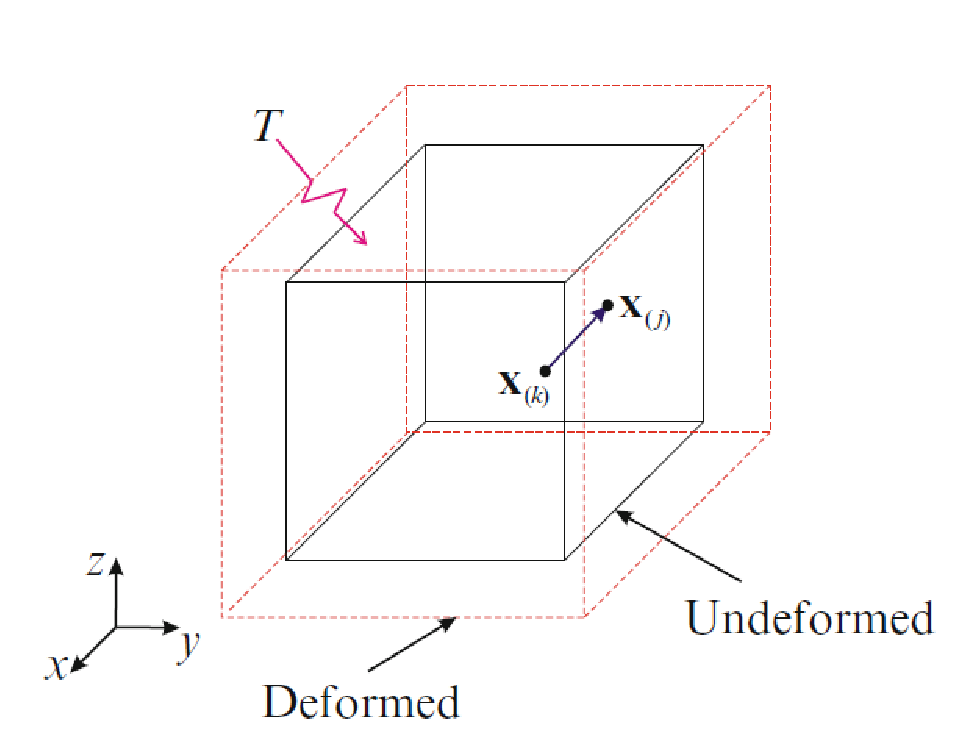
\includegraphics[width=0.5\linewidth]{chap/image/pdm_isotropic_expansion}

  \caption{\label{pdm_isotropic_expansion}
           各向均匀膨胀下的三维物体。图片取自\mycite{Madenci}{2014}。
          }
\end{figure}

在各向均匀膨胀下,应变张量为

\begin{eqnarray}
  \epsilon_{xx(k)} =  \epsilon_{yy(k)} = \epsilon_{zz(k)} = \zeta\\
  \epsilon_{xy(k)} =  \epsilon_{xz(k)} = \epsilon_{yz(k)} = 0
\end{eqnarray}

则经典连续介质力学中的应变能量密度 $W_{(k)}$ 和 膨胀度$\theta_{(k)}$ 可显式算得为

\begin{equation}
W_{(k)} = \frac{9}{2}\kappa\zeta^2\\
\label{eq:33}
\end{equation}
\begin{equation}
\theta_{(k)} = \epsilon_{xx(k)}+\epsilon_{yy(k)}+\epsilon_{zz(k)} = 3\zeta.
\label{eq:34}
\end{equation}

并且形变后的相对位置可用未形变空间的相对位置表示为

\begin{equation}
|\mb{y}_{(j)} - \mb{y}_{(k)}| = (1+\zeta)|\mb{x}_{(j)} - \mb{x}_{(k)}|.
\label{eq:35}
\end{equation}

定义 $\bm{\xi} = \mb{x}_{(j)} - \mb{x}_{(k)}$, $\xi = |\bm{\xi}|$。
最终,$W_{(k)}$ 和 $\theta_{(k)}$ 的计算需要在半径为 $\delta$ 的圆球内进行积分:

\begin{equation}
\begin{aligned}
W_{(k)} =& a\theta_{(k)}^2
           +b\sum_{j=1}^{N}\omega_{(k)(j)}(s_{(k)(j)}|\mb{x}_{(j)}-\mb{x}_{(k)}|V_{(j)})\cdot(s_{(k)(j)}|\mb{x}_{(j)}-\mb{x}_{(k)}|V_{(j)})\\
        =& a\theta_{(k)}^2
           +b\int_0^\delta\int_0^{2\pi}\int_0^{\pi}\frac{\delta}{\xi}\left[(1+\zeta)\xi-\xi\right]^2\xi^2\sin(\phi)d\phi d\theta d\xi\\
        =& 9a\zeta^2+\pi b\delta^5\zeta^2
\end{aligned}
\label{eq:36}
\end{equation}
和
\begin{equation}
\begin{aligned}
\theta_{(k)} =& d\sum_{j=1}^{N}\omega_{(k)(j)}s_{(k)(j)}\frac{\mb{y}_{(j)} - \mb{y}_{(k)}}{|\mb{y}_{(j)} - \mb{y}_{(k)}|}\cdot(\mb{x}_{(j)}-\mb{x}_{(k)})V_{(j)}\\
        =& d\int_0^\delta\int_0^{2\pi}\int_0^{\pi}\frac{\delta}{\xi}\left[(1+\zeta)\xi-\xi\right](\frac{\bm{\xi}}{\xi}\cdot\frac{\bm{\xi}}{\xi})\xi^2\sin(\phi)d\phi d\theta d\xi\\
        =& \frac{4\pi d\delta^4}{3}\zeta,
\end{aligned}
\label{eq:37}
\end{equation}

其中$(\xi,\theta,\phi)$ 为球坐标。将方程 \ref{eq:36},\ref{eq:37}同方程\ref{eq:33},\ref{eq:34}进行对比,则可以得到两个重要的关系式:

\begin{equation}
9a + \pi b\delta^5 = \frac{9}{2}\kappa
\label{eq:38}
\end{equation}
\begin{equation}
d = \frac{9}{4\pi\delta^4}.
\label{eq:39}
\end{equation}

\noindent{\textit{Case 2: 简单剪切}}

图\ref{pdm_simple_shear}所示为简单剪切形变下的三维物体。
\begin{figure}[htbp!]
  \centering
  \captionsetup{justification=centering}
  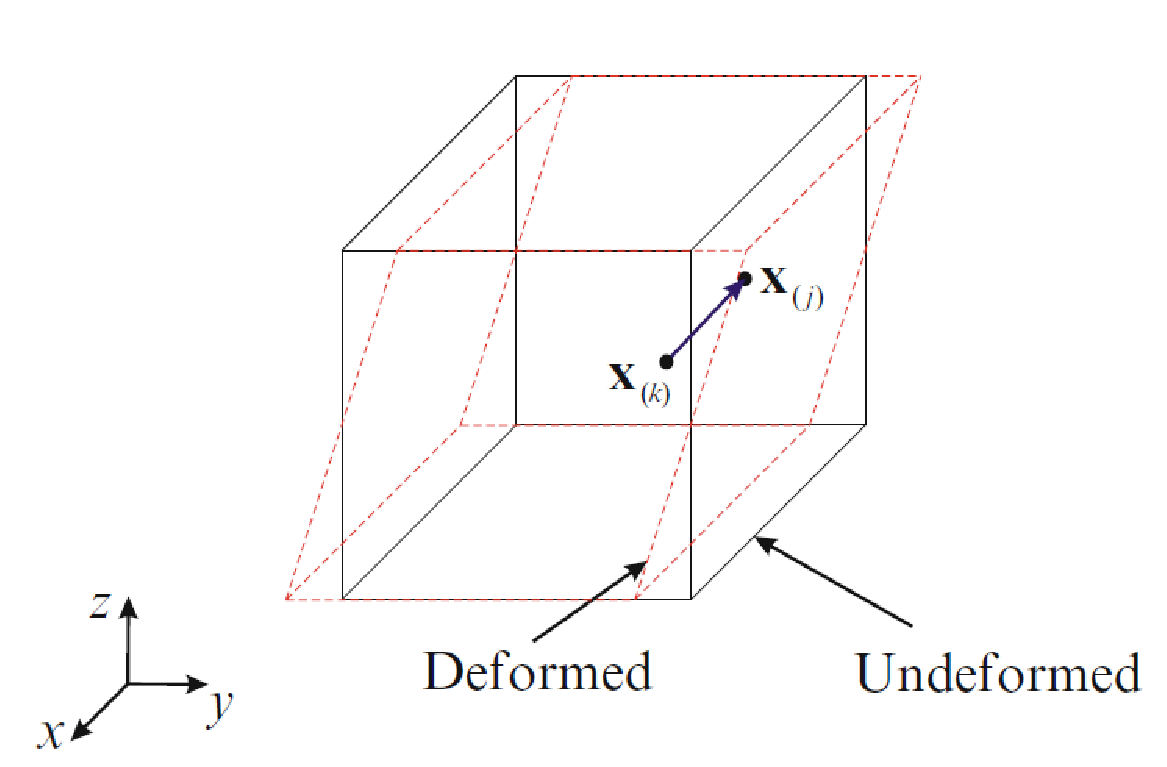
\includegraphics[width=0.5\linewidth]{chap/image/pdm_simple_shear}

  \caption{\label{pdm_simple_shear}
           简单剪切形变下的三维物体。图片取自\mycite{Madenci}{2014}。
          }
\end{figure}

在这种情形下,有类比关系:
\begin{equation}
\gamma_{xy(k)} = \zeta
\label{eq:40}
\end{equation}
\begin{equation}
\sigma_{xx(k)} = \sigma_{yy(k)} = \sigma_{zz(k)} = \gamma_{xz(k)} =\gamma_{yz(k)} = 0
\label{eq:41}
\end{equation}
及
\begin{equation}
|\mb{y}_{(j)} - \mb{y}_{(k)}| = (1+\frac{\zeta\sin(2\phi)\sin(\theta)}{2})|\mb{x}_{(j)} - \mb{x}_{(k)}|.
\label{eq:42}
\end{equation}

连续介质力学下的$W_{(k)}$ 和 $\theta_{(k)}$则可以直接写为

\begin{equation}
W_{(k)} = \frac{1}{2}\mu\zeta^2\\
\label{eq:43}
\end{equation}
\begin{equation}
\theta_{(k)} = 0.
\label{eq:44}
\end{equation}

近场动力学下的$W_{(k)}$的值仍然需要通过半径为 $\delta$ 的圆球内进行积分来计算。即
\begin{equation}
\begin{aligned}
W_{(k)} =& b\sum_{j=1}^{N}\omega_{(k)(j)}(s_{(k)(j)}|\mb{x}_{(j)}-\mb{x}_{(k)}|V_{(j)})\cdot(s_{(k)(j)}|\mb{x}_{(j)}-\mb{x}_{(k)}|V_{(j)})\\
        =& b\int_0^\delta\int_0^{2\pi}\int_0^{\pi}\frac{\delta}{\xi}\left[(1+\frac{\zeta\sin(2\phi)\sin(\theta)}{2})\xi-\xi\right]^2\xi^2\sin(\phi)d\phi d\theta d\xi\\
        =& \frac{b\pi\delta^5\zeta^2}{15}.
\end{aligned}
\label{eq:45}
\end{equation}

比较 \ref{eq:43} 和 \ref{eq:45} 获得:
\begin{equation}
b = \frac{15\mu}{2\pi\delta^5}.
\label{eq:46}
\end{equation}

将方程 \ref{eq:46} 代入 \ref{eq:38} 则可以获得 $a$ 的具体形式:
\begin{equation}
a = \frac{1}{2}(\kappa - \frac{5\mu}{3}).
\label{eq:47}
\end{equation}

到此为止,三个动力学参数($a, b, d$)已经全部确定。

\subsubsection{最终模型}

本章节已经推导了从经典连续介质力学到近场动力学理论,各向同性线性材料的本构模型的整个演变过程。为免读者混淆以及方便后续章节引用,在此我们做简要总结。在 ordinary state based 模型下,力密度的计算通过如下方式计算:

\begin{equation}
\tkj = \frac{1}{2}A\frac{\bfyj - \bfyk}{|\bfyj - \bfyk|}
\label{eq:48}
\end{equation}
其中
\begin{equation}
A = 4\wkj\left\{ad\frac{\bfyj-\bfyk}{|\bfyj-\bfyk|}\cdot\frac{\bfxj-\bfxk}{|\bfxj-\bfxk|}\thetak
   +b\left(|\bfyj - \bfyk| - |\bfxj - \bfxk|\right) \right\}
\label{eq:49}
\end{equation}
\begin{equation}
\thetak = d\sum_{j=1}^{N}\wkj\skj\frac{\bfyj - \bfyk}{|\bfyj - \bfyk|}\cdot(\bfxj-\bfxk)V_{(j)}
\label{eq:50}
\end{equation}
\begin{equation}
a = \frac{1}{2}(\kappa - \frac{5\mu}{3})
\label{eq:51}
\end{equation}
\begin{equation}
b = \frac{15\mu}{2\pi\delta^5}
\label{eq:52}
\end{equation}
\begin{equation}
d = \frac{9}{4\pi\delta^4}
\label{eq:53}
\end{equation}


    \chapter{PDM之形变模拟}

\section{弹性模型}
\label{elasitcity_model}

在章节\ref{pdm_derivation}中,本文已经推导了近场动力学中关于线性材质的各向同性模型,其具体形式由式 \ref{eq:48}$\sim$\ref{eq:53} 所示。同时本文还给出了关于一般超弹性模型的推导框架,以应用于其他材质模型。考虑到线性模型的简单性,所以在本文工作中主要采用了这一模型。但从式 \ref{eq:48}$\sim$\ref{eq:53}给出的模型可以看出,其在理解上仍然不够具有物理直观,因此在本章节将对其进行重新表述,并给出所用超弹性模型的最终版本。

如前章节所述,在近场动力学中,由粒子 $j$ 施加给粒子 $i$ 的弹性内力密度可具体写为
\begin{equation}
\mathbf{T}\langle\mathbf{x}_j,\mathbf{x}_i\rangle = \frac{1}{2}A\frac{\mathbf{y}_j-\mathbf{y}_i}{|\mathbf{y}_j-\mathbf{y}_i|}
\end{equation}

其中 $\mathbf{x}$ 和 $\mathbf{y}$ 分别是粒子形变前和形变后的位置,力密度的方向即为粒子之间的连线方向,由$\frac{\mathbf{y}_j-\mathbf{y}_i}{|\mathbf{y}_j-\mathbf{y}_i|}$给定。$A$ 则代表力的大小,其包含所有的本构信息,并由式 \ref{eq:49} 给出(注意下标有所改变)

\begin{equation}
A = 4\omega_{ij}\left\{ad\frac{\mb{y}_j-\mb{y}_i}{|\mb{y}_j-\mb{y}_i|}\cdot\frac{\mb{x}_j-\mb{x}_i}{|\mb{x}_j-\mb{x}_i|}\theta_i
   +b\left(|\mb{y}_j - \mb{y}_i| - |\mb{x}_j - \mb{x}_i|\right) \right\}
\end{equation}

事实上,可以将其分解为各向均匀膨胀项(dilatational part)和剪切项(deviatoric part),从而更具有物理直观。为完成这一目标,首先需要将参数 $a$ 分解为两个部分:

\begin{equation}
a = a_1 + a_2 \qquad \mathrm{with}\quad a_1 = \frac{1}{2}\kappa ,\quad a_2 = -\frac{5\mu}{6}
\end{equation}

需要额外注意的是,当泊松比为 0.25 时,$a$ 等于 0。在此情形下,膨胀度 $\theta_i$ 将消失,模型将回退到 bond based 情形,整个系统实际上也将退化为质点弹簧系统。不难看出 $\theta_i$ 的引入是区分bond based 模型和 state based 模型的关键。将 $a$ 分解后,便可以将 $A$ 重新整理为

\begin{equation}
\begin{aligned}
A =4\omega_{ij}\left\{a_1d\frac{\mb{y}_j-\mb{y}_i}{|\mb{y}_j-\mb{y}_i|}\cdot\frac{\mb{x}_j-\mb{x}_i}{|\mb{x}_j-\mb{x}_i|}\theta_i
   +b\left(e_{ij} + \frac{a_2d}{b}\frac{\mb{y}_j-\mb{y}_i}{|\mb{y}_j-\mb{y}_i|}\cdot\frac{\mb{x}_j-\mb{x}_i}{|\mb{x}_j-\mb{x}_i|}\theta_i\right) \right\}
\end{aligned}
\end{equation}

其中$e_{ij} = |\mb{y}_j - \mb{y}_i| - |\mb{x}_j - \mb{x}_i|$为粒子之间的伸长量,其相当于连续介质力学中的柯西应变张量。注意在花括号中,第一项仅仅和体积模量 $\kappa$ 和膨胀度 $\theta_i$ 相关,而第二项仅仅和剪切模量 $\mu$ 相关。因此,上式已经成功将形变分解为膨胀项和剪切项两个部分。对于剪切项,可以进一步定义剪切伸长分量(deviatoric component of extension):

\begin{equation}
\begin{aligned}
e^d_{ij} \equiv& e_{ij} + \frac{a_2d}{b}\frac{\mb{y}_j-\mb{y}_i}{|\mb{y}_j-\mb{y}_i|}\cdot\frac{\mb{x}_j-\mb{x}_i}{|\mb{x}_j-\mb{x}_i|}\theta_i\\
                  =& e_{jk} - \frac{\delta}{4}\frac{\mb{y}_j-\mb{y}_i}{|\mb{y}_j-\mb{y}_i|}\cdot\frac{\mb{x}_j-\mb{x}_i}{|\mb{x}_j-\mb{x}_i|}\theta_i
\end{aligned}
\label{deviatoric_extension}
\end{equation}

从直观上看,$e^d_{ij}$ 相当于是移除总形变 $e_{ij}$ 中的各向均匀碰撞部分。经上述分解后,力密度大小 $A$ 可以最终写为

\begin{equation}
A = A_{dil} + A_{dev}
\end{equation}
其中 $A_{dil}$ 和 $A_{dev}$ 即分别为力密度大小的各向均匀膨胀部分以及剪切形变部分:
\begin{equation}
A_{dil}=4\omega_{ij}a\frac{\mathbf{y}_j-\mathbf{y}_i}{|\mathbf{y}_j-\mathbf{y}_i|}\cdot\frac{\mathbf{x}_j-\mathbf{x}_i}{|\mathbf{x}_j-\mathbf{x}_i|}\theta_i
\end{equation}

\begin{equation}
A_{dev}=4\omega_{ij}b(e_{ij}-\frac{\delta}{4}\frac{\mathbf{y}_j-\mathbf{y}_i}{|\mathbf{y}_j-\mathbf{y}_i|}\cdot\frac{\mathbf{x}_j-\mathbf{x}_i}{|\mathbf{x}_j-\mathbf{x}_i|}\theta_i)
       =4\omega_{ij}be^d_{ij}
\label{Adev}
\end{equation}

注意在上式中,动力学参数 $a$ 已经被重新定义。近场动力学的两个动力学参数 $a$,$b$ 的作用实际上相当于连续介质力学中的体积模量和剪切模量,甚至因为近场动力学由连续介质力学演变而来,这两个参数可以直接由体积模量及剪切模量表示:

\begin{equation}
a \equiv a_1d = \frac{9\kappa}{8\pi\delta^4} ,\qquad b = \frac{15\mu}{2\pi\delta^5},
\end{equation}

上式中 $a$ 仅和 $\kappa$,而 $b$ 仅和 $\mu$ 相关。膨胀度 $\theta_i$ 、伸长比 $s_{ik}$(stretch)和权重函数仍然维持原有定义,具体写为

\begin{equation}
s_{ik}=\frac{|\mathbf{y}_k-\mathbf{y}_i|}{|\mathbf{x}_k-\mathbf{x}_i|} -1
\end{equation}

\begin{equation}
\omega_{ij} = \frac{\delta}{|\mathbf{x}_j-\mathbf{x}_i|}
\end{equation}

\begin{equation}
\theta_i = \frac{9}{4\pi\delta^4}\sum_{k=1}^N\omega_{ik}s_{ik}\frac{\mathbf{y}_k-\mathbf{y}_i}{|\mathbf{y}_k-\mathbf{y}_i|}\cdot(\mathbf{x}_k-\mathbf{x}_i)V_k
\end{equation}

$s_{ik}$ 衡量的是粒子间 bond 的伸长量。 $\omega_{ij}$ 为权重函数,其是单调递减的,即离中心粒子 $i$ 越近,则权重越大。注意 $\omega_{ij}$ 定义在材质空间(material space)而不是形变空间,因此其值取决于粒子的初始分布。最后,$\theta_i$ 衡量的是粒子 $i$ 所在位置的各向均匀膨胀度,其通过粒子 $i$ 的位置和其邻域范围内的其他粒子 $k$ 的位置来算得。仔细考虑可以发现,$\theta_i$ 的引入将使得粒子 $i$ 和粒子 $j$ 的相互作用力不仅仅和彼此相关,而是和粒子的整个邻域范围内的其他粒子相关。在使用基于显式欧拉积分的方法中(章节\ref{explicit_euler_method}),付出的代价仅仅是为每一个粒子,都计算其 $\theta_i$ 值,整体上并不改变算法的复杂度。但对于隐式欧拉方法(章节\ref{implicit_euler_method}),情况则不同。因为刚度矩阵 $\textbf{K} = \frac{\partial \textbf{f}^{int}}{\partial \textbf{x}}$ 的计算同样需要考虑整个邻域,因而给整个算法的实现额外增加了一层复杂度,因此在较大规模仿真系统中,直接使用隐式欧拉积分以当前计算能力仍难具可行性。

\section{塑性模型}
塑性形变表示的是当材料的形变过大时,由于材料内部的屈服而导致无法回退到最开始的未形变状态,物质的内部结构被永久改变。
由于塑性行为的复杂性,现阶段关于近场动力学理论中塑性模型的研究仍然屈指可数。\mycite{Silling}{2007}在其工作中第一次提出了一个适用于近场动力学理论的塑性模型,这一模型在原理上类似经典理论中的 von Mises 流动模型。 Mitchell et al. 则根据这一模型,提出了一个关于近场动力学塑性行为的仿真框架\mycite{Mitchell}{2011}。但据本文所知,到目前为止,这一模型在学术界仅仅是停留在理论分析层面,而并没有相关工作对其进行验证。本文工作应为第一次在实际应用中使用这一模型,但同时针对图形学的应用特点做出了一些针对性的修改。

本文所用模型基于纯粹的剪切塑性流动理论(purely deviatoric plastic flow theory),即塑性仅跟剪切形变有关。因此我们需要将式\ref{deviatoric_extension}定义的剪切伸长量以加法形式分解为两部分:

\begin{equation}
e_{ij}^d = e_{ij}^e+e_{ij}^p
\end{equation}

其中 $e_{ij}^e$ 和 $e_{ij}^e$ 分别为剪切应变中的弹性部分和塑性部分。为将塑性模型集成进入原有的近场动力学弹性本构模型,我们需要将内力密度大小 $A$ 的剪切分量 $A_{dev}$(见式 \ref{Adev})重新定义为

\begin{equation}
A_{dev} = 4\omega_{ij}b(e_{ij}^d-e_{ij}^p)
\end{equation}

上式的目的是在进行力计算时,将塑性形变部分从总的剪切形变部分中移除。对于弹性模型,则项 $e_{ij}^p$ 直接消失,上式回退到方程\ref{Adev}。$e_{ij}^p$ 是模拟塑性的最关键的部分,而塑性行为的仿真仿真需要两大关键步骤。第一是在仿真时物体形变的过程中,判断物体是否由弹性进入到塑性状态。第二则是需要根据形变的大小,更新总剪切形变中的塑性部分。

对于判断塑性是否发生,一般使用的是屈服方程 $f(A_{dev})$ (yield function)来进行决定:

\begin{equation}
f(A_{dev}) = \frac{(A_{dev})^2}{2}-\Psi_0,
\end{equation}

其中 $\Psi_0$ 代表进入塑性状态的阈值,值越大代表塑性愈难发生,而越小则代表物体更容易发生塑性形变。在上式中,如果$f(A_{dev})\leq 0$ 则处于弹性状态,而如果 $f(A_{dev}) > 0$,则意味着材料将发生塑性行为。

在塑性形变发生的情形下,需要重新计算物体所受的剪切力部分(膨胀项部分不受影响)。为此,我们需要将 $A_{dev}$ 投影于屈服平面之上以获取真正的剪切力密度,即

\begin{equation}
A_{dev}^c=\sqrt{2\Psi_0}\mathrm{sign}(A_{dev}),
\end{equation}

其中 $\mathrm{sign}(\cdot)$ 为符号方程。$A_{dev}^c$ 的值可进一步用于更新塑性形变部分 $e^p$ 的更新,如下

\begin{equation}
\triangle e_n^p = \frac{1}{2b}(A_{dev}-A_{dev}^c)
\end{equation}
\begin{equation}
e_{n+1}^p = (e_n^p+\triangle e_n^p)\mathrm{min}\big(1,\frac{\gamma}{|e_n^p+\triangle e_n^p|}\big).
\end{equation}

在上式中下标 $n$ 和 $n + 1$ 分别表示当前时间步和下一时间步。在时间步 $n$ 时,可以算得总的弹性形变量,当前塑性形变由前续仿真步累计而来,因此可以算得当前塑性形变部分的增量。注意,上式中的 $\gamma$ 参数用来对塑性的总量进行限制,这一参数并没有出现在\mycite{Mitchell}{2011}所提出的模型中,而是本文借鉴了\textcolor{blue}{(O'Brien et al. 2002)\parencite{OBrien2002}}所提出的加法模型,设计了此参量。实验证明,在引入此参量之后,可以获得对于塑性行为更多的控制,以及对于仿真的稳定性也大有裨益。但值得注意的是,这一参数的引入并不符合真正的材料属性,即使在发生极大塑性形变行为下,材料也不可能重新进入弹性状态,因此 $\gamma$ 参数更多的是防止仿真过程中由于数值抖动而引起整个仿真崩溃。本文所用的塑性模型可总结为如图\ref{plasticity_model}所示:

\begin{figure}[!htb]
  \centering
  \captionsetup{justification=centering}
  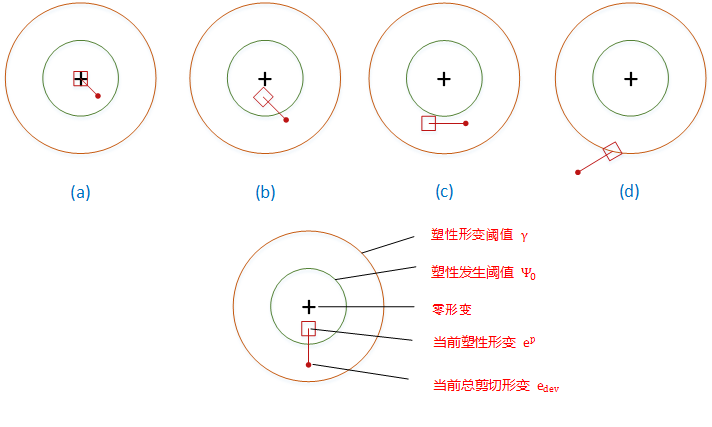
\includegraphics[width=\linewidth]{chap/image/plasticity_model}

  \caption{\label{plasticity_model}
           塑性模型示意图。其中图(a)为弹性形变,图(c)和图(c)为塑性形变,图(d)表示超出塑性形变总量限制。
          }
\end{figure}


\section{离散化框架及嵌网格策略}
\label{discretization}

尽管基于粒子的无网格方法在物理计算上较为灵活方便,但付出的代价就是需要重新产生网格来进行表示。不同于工程领域只关注于计算的准确性,图形学领域中的应用实际上更关注视觉效果,所以炫酷的视觉渲染输出尤为重要。纯粹使用基于粒子的方法来进行渲染在流体仿真中较为常见,例如可以使用基于屏幕空间(Screen-based)的渲染技术来取得不错的效果。但现有应用的视觉输出大部分都是采用基于网格(mesh)的渲染达到的,甚至对于高质量的流体渲染,通常的方式也是离线将粒子云使用相关算法来重建网格,如 Marching Cube 等。但重建网格的方式对于固体仿真尤其是碎裂仿真几乎是不可能的,因为纯粹基于粒子位置信息很难对裂纹进行重建和复原。因此,更常见的方式是采用嵌网格的办法来对物体的形变和碎裂进行显式追踪,本文工作亦使用这种方式。

使用嵌网格方法的优点是网格的边界即代表物体的表面,因此在渲染时能够提供更多的细节,并且也比较容易反映仿真过程中物体的形变以及碎裂。在本文工作中,我们直接使用四面体网格来离散整个仿真物体,并且将仿真粒子置于四面体的几何中心,亦即每一个四面体即代表一个仿真粒子,如图\ref{embedded_mesh}所示。

\begin{figure}[!htb]
  \centering
  \captionsetup{justification=centering}
  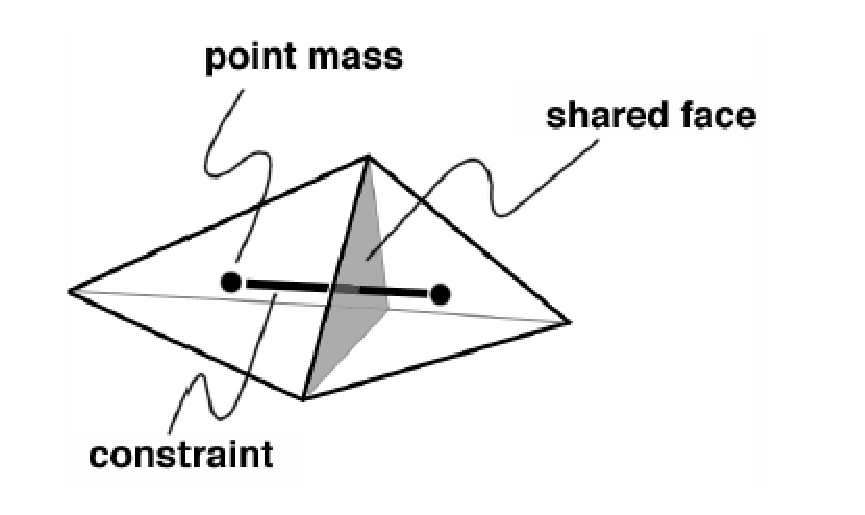
\includegraphics[width=0.6\linewidth]{chap/image/embedded_mesh}

  \caption{\label{embedded_mesh}
           离散化框架与嵌网格。本文工作将仿真粒子置于四面体的中心,相邻的粒子共享一个四面体表面,并且粒子之间通过 bond 相连。
          }
\end{figure}

在将仿真粒子置于网格单元体的中心后,便可以根据设定的邻域半径 $\delta$ 来对每一个粒子的邻域 $H_\mb{x}$(family)进行初始化。关于搜寻邻域范围内的粒子,比较 naive 的方式是直接双重循环遍历,计算粒子对之间距离,然后判断是否位于其邻域范围内,如此整个算法的复杂度为 $O(N^2)$。 但更具效率的方式是进行空间哈希,将粒子先置于均匀分布的空间栅格(grid)中,然后针对每一个 grid,只需要搜寻其周围 27 个直接相邻的栅格中粒子,然后判断是否位于邻域半径 $\delta$ 内即可,这一算法几乎是 $O(N)$ 的,从而能大幅度提高粒子搜寻的效率。不过,粒子的邻域初始化工作位于仿真开始之前的预处理阶段,对于包含四面体数较少的物体,使用 $O(N^2)$ 并不影响整体仿真效率。

在物体发生形变之后,便需要对于拓扑网格进行更新,其需要改变四面体网格中顶点的位置。本文工作所采用的方法是根据基于连接该顶点的四面体中的仿真粒子位置,以加权平均的方式来进行更新,具体而言:

\begin{eqnarray}
\omega_{\mathrm{v}} &=& \sum_{\mathrm{p}} \frac{1}{4}m_{\mathrm{p}}\\
\textbf{v}_{\mathrm{v}} &=& \frac{1}{\omega_{\mathrm{v}}}\sum_{\mathrm{p}}\frac{1}{4}m_{\mathrm{p}}\textbf{v}_{\mathrm{p}}\\
\mathbf{x}_{\mathrm{v}}^{t+1} &=& \mathbf{x}_{\mathrm{v}}^{t} + \Delta t\textbf{v}_{\mathrm{v}}
\end{eqnarray}

其中下标 $\mathrm{p}$ 和 $\mathrm{v}$ 分别表示粒子(particle)和网格顶点(vertex),$m_{\mathrm{p}}$ 和 $\textbf{v}_{\mathrm{p}}$ 分别是粒子的质量和速度,$\textbf{v}_{\mathrm{v}}$ 和 $\textbf{x}_{\mathrm{v}}$分别是网格顶点的速度和位置。在具体实现时,并不需要逐顶点来进行更新,因为一般不针对每一顶点存储与其相连的四面体,而可以直接通过遍历全部四面体,然后将四面体的四个顶点的权值和速度分别累加,累加完所有权值和速度之后,再遍历顶点将累加的速度除以权值即可。

值得注意的是,如果仅针对形变体问题,将仿真粒子置于四面体中心其实并不直观,并且随着仿真的进行,仿真粒子并不完全位于四面体的中心,而是会有所偏离。虽然在本文工作的实验中,并未发现明显的异常情况,但实际上在极大形变下,这一缺陷可能会体现出来。更为简单的方式是直接令仿真粒子对应到四面体的顶点上,这样粒子位置即顶点位置,处理起来更为方便。本文工作采用此种离散方式的理由是为了方便后续的碎裂引起的拓扑网格更新,其不仅仅是改变顶点的位置,还需要直接改变网格的拓扑结构,因为近场动力学的碎裂实质上是 bond 的消除,如果将仿真粒子对应到顶点则很难在四面体网格上进行体现,详见章节xxx。



\section{实验结果}
\label{deformation_results}

本文工作所有实验(包括碎裂仿真实验,见章节\ref{fracture_results})都运行于一台 CPU 配置为 3.5GHz, Intel Core i7-5930,内存为 32GB 的主机。实验所用的物体模型由开源软件 TetGen 生成\mycite{Si}{2015}之上,其可以直接通过给定粒子云或者给定 .Obj 格式的表面网格来产生高质量四面体网格。而最终的渲染输出,都是直接从四面体网格中提取表面网格,使用 POV-Ray \footnote{http:www.povray.org/} 开源光线追踪软件并配置相关光照参数渲染而成。

本文工作所有实现基于前述章节所述的近场动力学弹塑性模型,以及后续章节将要阐述的碎裂和各向异性模型,并且使用 openMP 来进行多线程实现。本章节将主要阐述基于 PDM 方法产生形变仿真效果。

为确保所用本构模型的正确性,本文实验通过多样化材质的属性参数来分别进行仿真实验,并和 FEM 方法进行了充分的对比。
其中图\ref{demo_pull_armadillo} 所示为 Armadillo 的各向同性线性形变实验。初始时 Armadillo 四肢被固定,并且其背部拉扯到一定位置,松开后 Armadillo 便往前振荡。可以看到即使 Armadillo 四肢被过度拉伸,但并没有产生明显的数值塑性,整个形变过程非常自然。


\begin{figure}[!htb]
  \centering
  \captionsetup{justification=centering}
  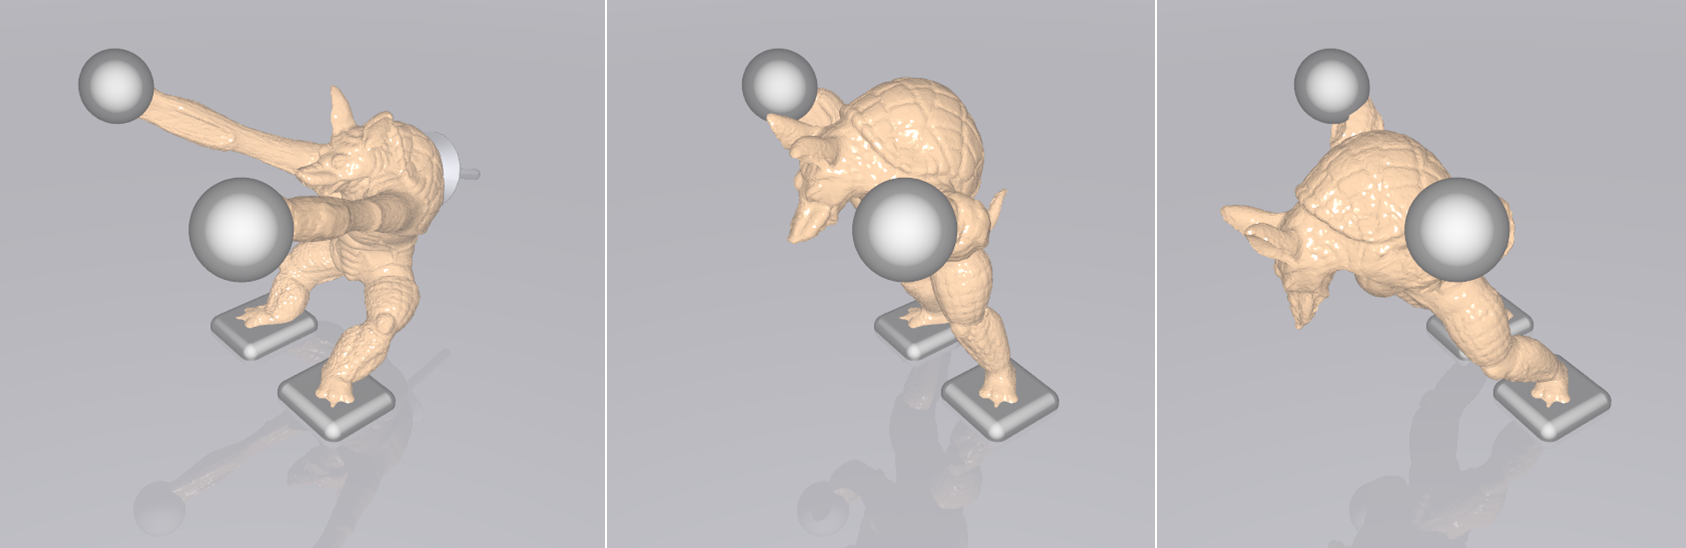
\includegraphics[width=0.9\linewidth]{chap/image/demo_pull_armadillo}

  \caption{\label{demo_pull_armadillo}
           Armadillo 各向同性线性形变实验。初始时 Armadillo 四肢被固定,并且其背部拉扯到一定位置,然后松开。
          }
\end{figure}

在图\ref{demo_impact_upside}的实验中,本文比较了物体的弹性形变和塑性形变行为。不同材质的物质被以恒定速度运行球从上沿方向撞击。其中弹性物体被撞击后发生形变,并能恢复到初始状态。塑性物体被撞击后会发生塑性形变,但并不能恢复到原始位置。

\begin{figure}[!htb]
  \centering
  \captionsetup{justification=centering}
  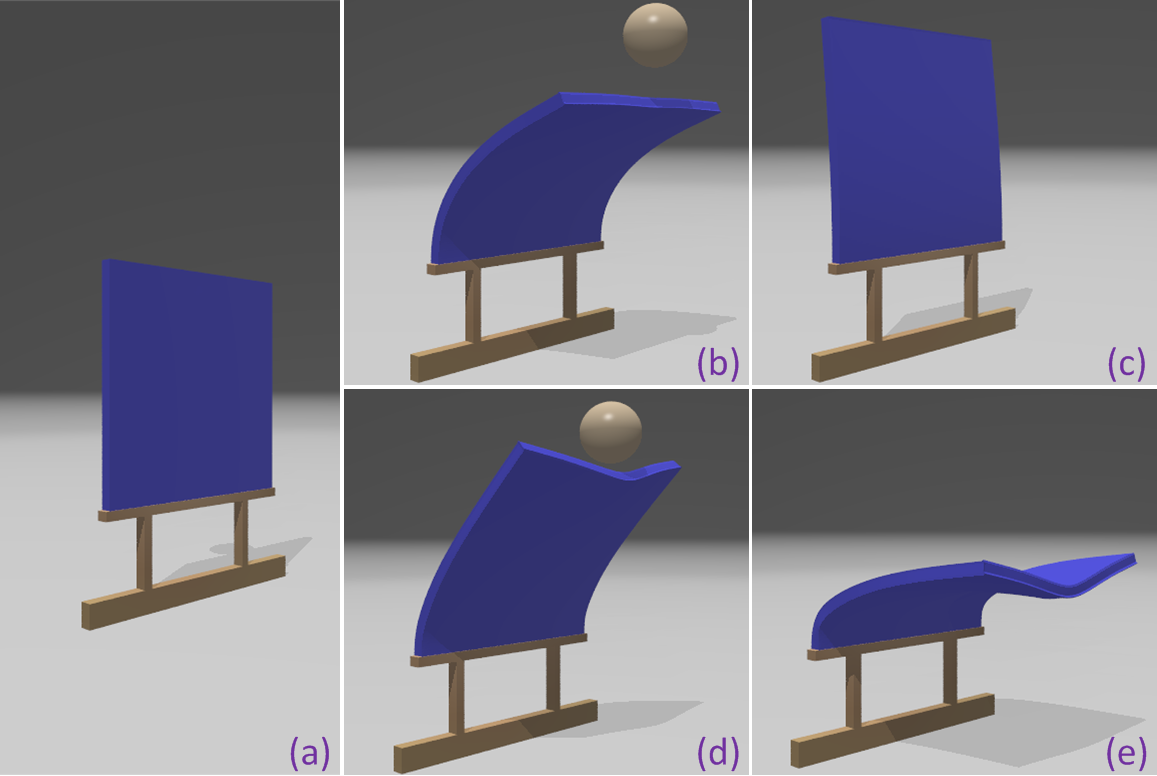
\includegraphics[width=0.7\linewidth]{chap/image/demo_impact_upside}

  \caption{\label{demo_impact_upside}
           弹性形变和塑性形变对比实验。不同材质的物质被以恒定速度运行球从上沿方向撞击。图(a)表示相同的初始状态。图(c)表示弹性物体被撞击,然后发生形变,但是在图(c)中,形变被恢复。图(d)表示物体被撞击后发生塑性形变,并且如图(e)所示,并不能恢复到原始位置。
          }
\end{figure}

图\ref{compare_different_poisson_ratio}则是对弹性材料(伸长的 beam)不同泊松比的对比实验。在 bond based 模型中,泊松比被固定为 0.25,如\mycite{Levine}{2014}。而使用基于 state based的模型能够破除这一限制,在材质属性的表达能力上达到同连续介质理论同等的水平。

\begin{figure}[!htb]
  \centering
  \captionsetup{justification=centering}
  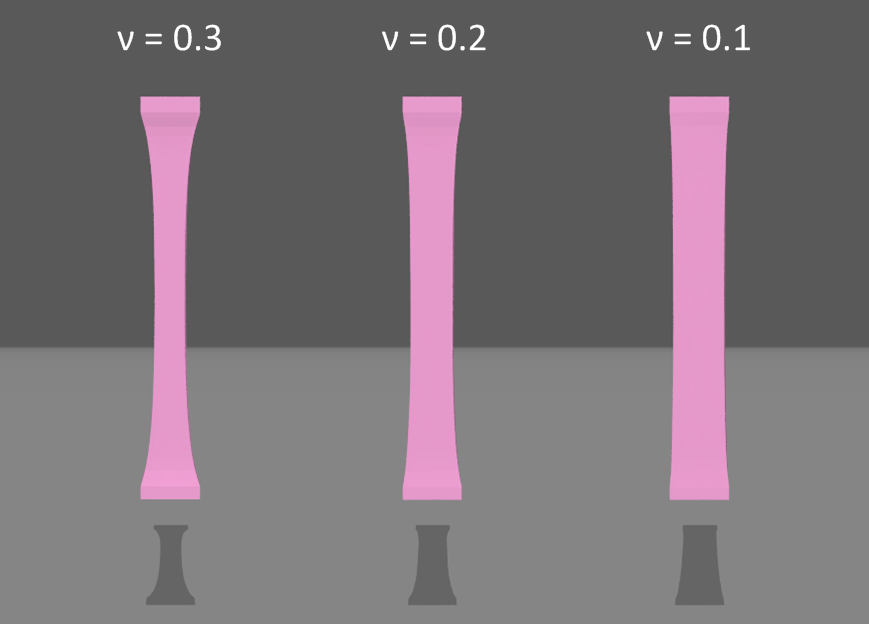
\includegraphics[width=0.7\linewidth]{chap/image/compare_different_poisson_ratio}

  \caption{\label{compare_different_poisson_ratio}
           不同泊松比对比实验。泊松比越大,则不可压性质越明显。
          }
\end{figure}

最后,本文进行了四组同 FEM 的对比实验。其中图\ref{demo_strip_vs_fem}为长条在重力下的弯曲实验。可以看到,近场动力学方法和 FEM 方法取得了几乎一致的效果。

\begin{figure}[!htb]
  \centering
  \captionsetup{justification=centering}
  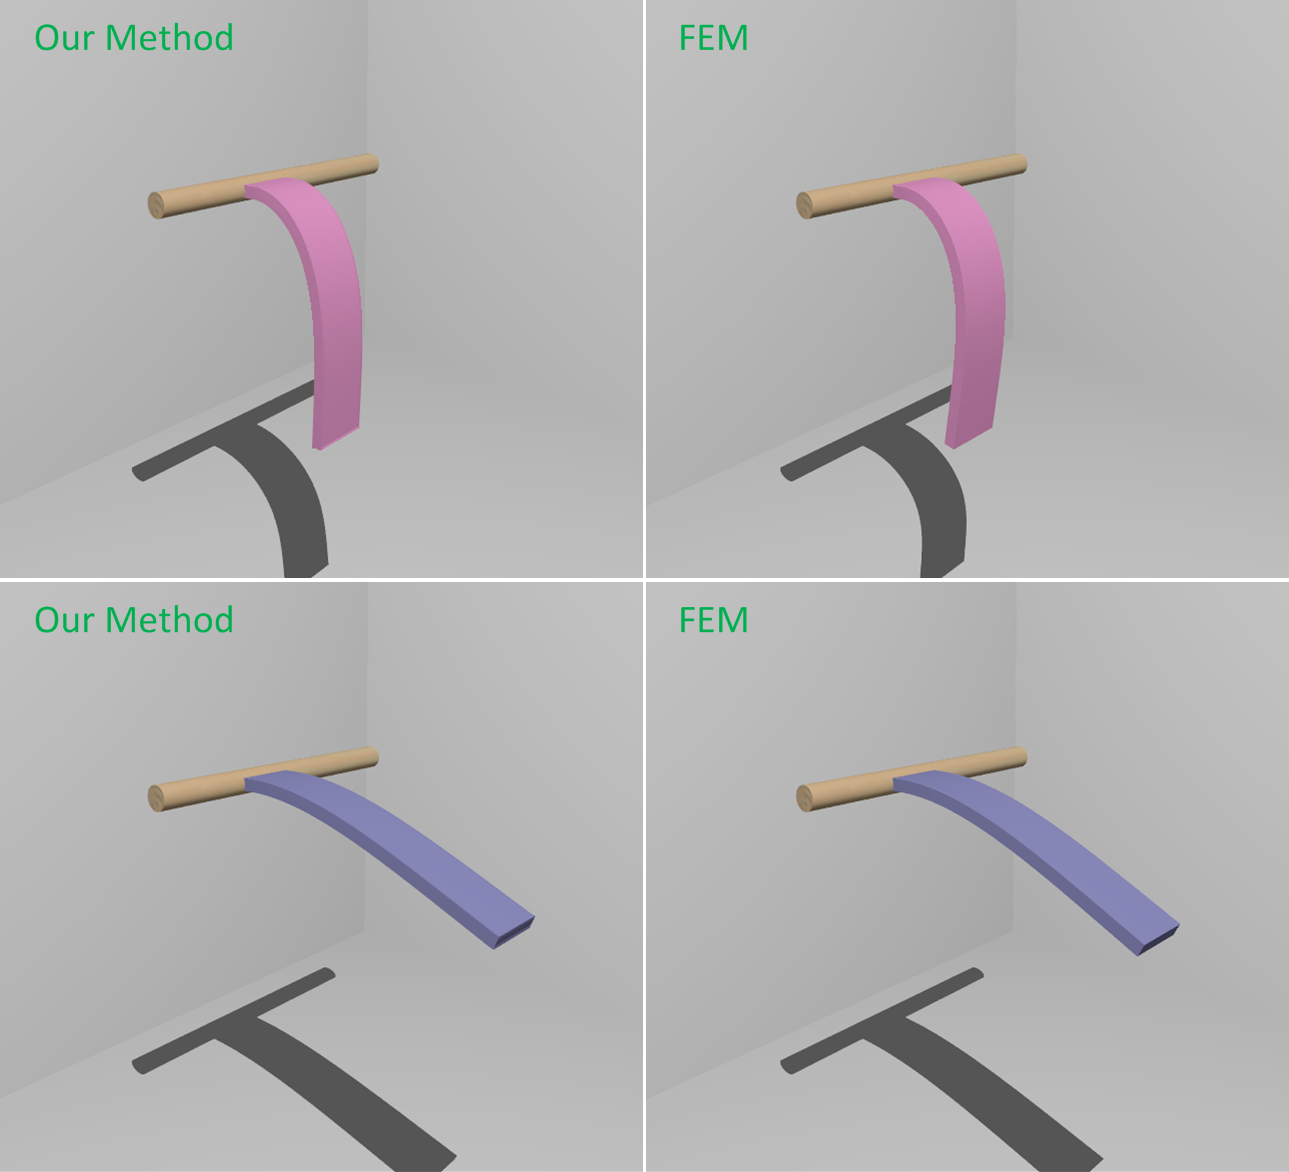
\includegraphics[width=0.7\linewidth]{chap/image/demo_strip_vs_fem}

  \caption{\label{demo_strip_vs_fem}
           不同硬度的长条弯曲实验。左边为本文方法所取得的效果,右图为 FEM 方法效果。可以看到,两者取得了几乎一致的效果。
          }
\end{figure}

图\ref{demo_bar_oscillate_vs_fem}所示实验为晃动的 Bar。仿真初始时, Bar 被摆到一定角度位置,然后松开发生晃动。对于这种大形变行为,可以显著感受到使用线性弹性模型的 FEM 方法将出现明显的不自然行为。并且可以看出,本文所提的线性近场动力学模型和 FEM 中的共旋线性模型在效果上几乎完全一致。本文进一步对两者的误差进行衡量,发现两者位置偏离小于 10\%。其中位置偏移通过 $Error = \frac{|\bm{x}_p-\bm{x}_p^{ref}|}{d}$ 定量衡量,其中 $d$ 为物体包围盒的对角长度。

\begin{figure}[!htb]
  \centering
  \captionsetup{justification=centering}
  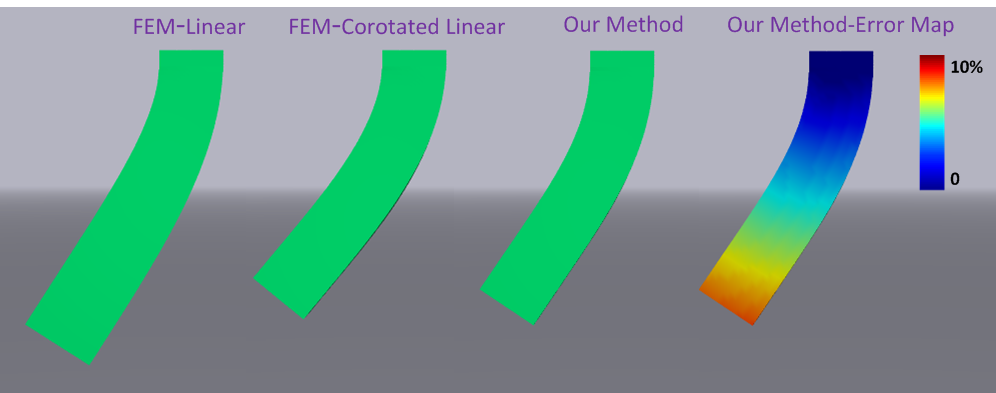
\includegraphics[width=0.9\linewidth]{chap/image/demo_bar_oscillate_vs_fem}

  \caption{\label{demo_bar_oscillate_vs_fem}
           Bar 晃动实验。最左图为 FEM 线性模型,可以看到明显的不自然现象。中间两图分别为共旋线性模型和近场动力学方法,两者效果几乎完全一致。右图为误差图,基本上小于 10\%。
          }
\end{figure}

从效果上看,近场动力学中的线性模型要远好于 FEM 中的线性模型,并且可以取得和 FEM 中的共旋线性模型相比的效果。原因在于其并没有使用 FEM 中柯西应变张量,因此并不是几何线性中的。进一步而言,在近场动力学中,纯粹的刚性变化并不会像 FEM 中的线性模型一样,产生虚拟的力(ghost force),从而大程度地拓展了近场动力学模型的适用范围。在图\ref{demo_bar_twist_vs_fem}中,本文还对扭曲的 Bar 进行对比实验,从图中可以更明显的看出 FEM 线性模型的缺陷。图\ref{demo_armadillo_vs_fem}展示为 Armadillo 复杂的周期性振荡形变行为,可以看到,在如此复杂的形变行为上,近场动力学仍然取得了和 FEM 非常一致的效果。

\begin{figure}[!htb]
  \centering
  \captionsetup{justification=centering}
  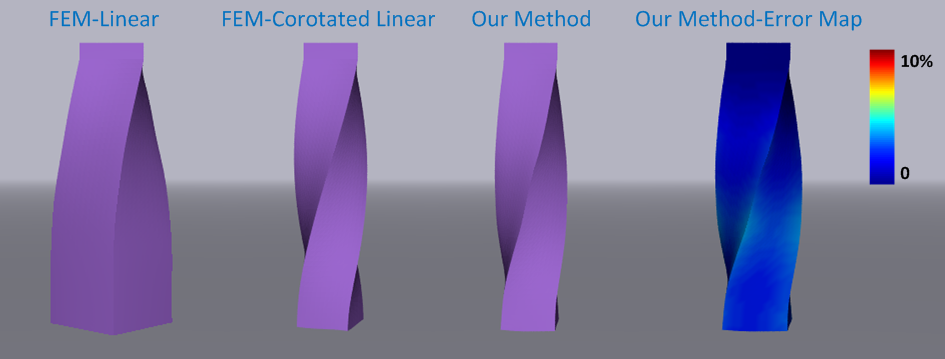
\includegraphics[width=0.9\linewidth]{chap/image/demo_bar_twist_vs_fem}

  \caption{\label{demo_bar_twist_vs_fem}
           Bar 扭曲实验。最左图为 FEM 线性模型,可以看到更为明显的不自然现象。中间两图分别为共旋线性模型和近场动力学方法,两者效果几乎完全一致。右图为误差图,基本上小于 10\%。
          }
\end{figure}

\begin{figure}[!htb]
  \centering
  \captionsetup{justification=centering}
  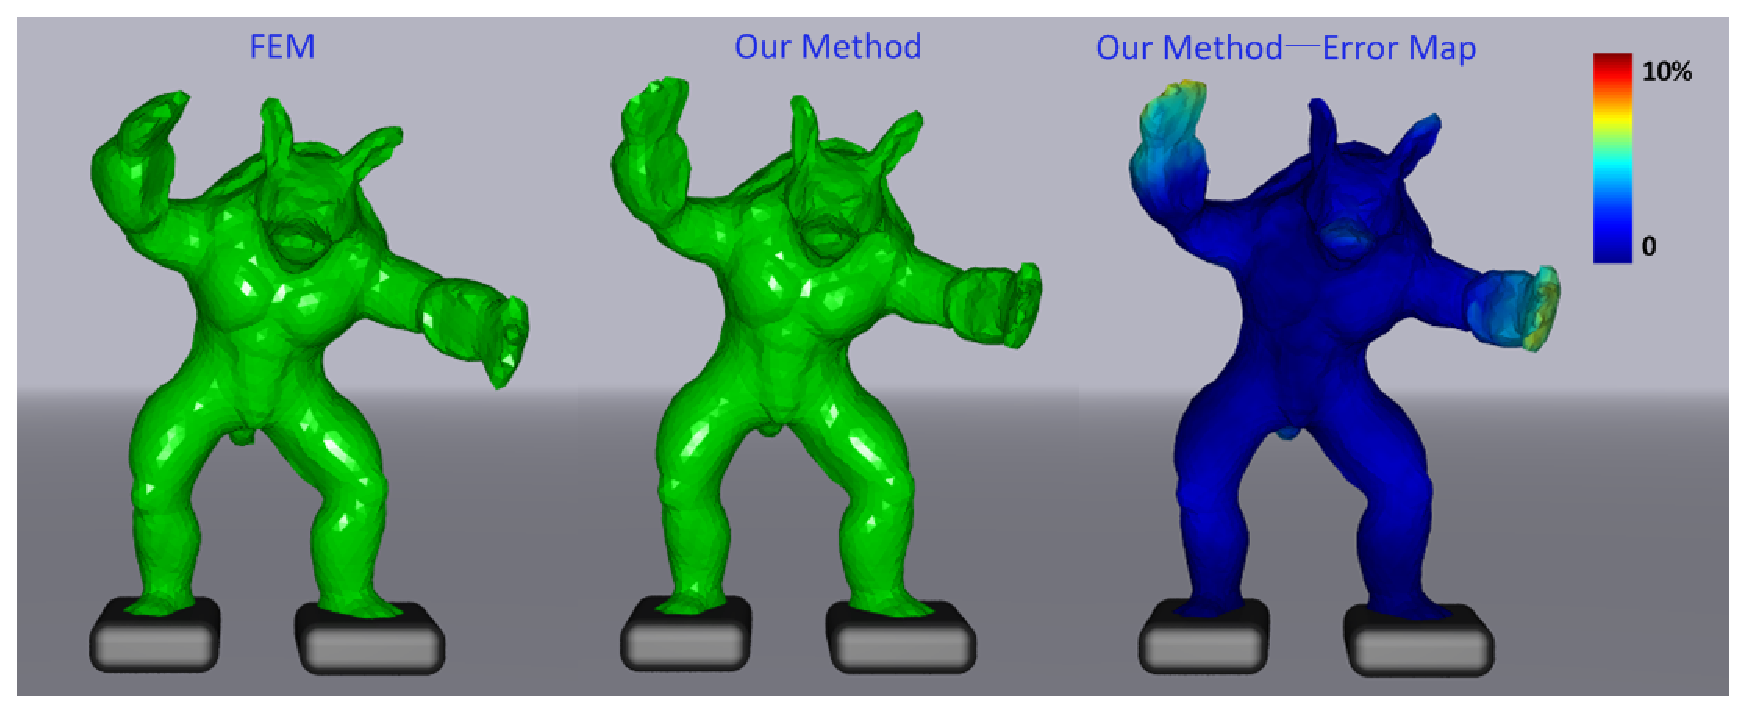
\includegraphics[width=0.9\linewidth]{chap/image/demo_armadillo_vs_fem}

  \caption{\label{demo_armadillo_vs_fem}
           Armadillo 周期性振荡实验。左图为 FEM 方法,中图为近场动力学方法,右图为误差图。即使对于这种复杂的周期性振荡形变行为,两者仍然取得了非常一致的效果。
          }
\end{figure}

下表\ref{deformation_results_table}展示了上述形变仿真实验所有模型参数以及物理参数。从表中所示数据来看,近场动力学方法能够取得和 FEM 类似的计算效率,但近场动力学方法相对更易实现以及并行化。

\begin{table*}[htb]
\centerline{
\resizebox{1.3\textwidth}{!}{
\begin{tabular}{lccccccccccccc}
  \hline
  \hline
  Examples & particle num & $\delta$ & bond num & $\kappa$ & $\mu$ & $\rho$            & $\Psi_0$ & $\frac{\gamma}{|\mathbf{x}_j-\mathbf{x}_i|}$ & $s^w_{(k)(j)}$ & $\Delta t$ &$\lambda_a$    & $\lambda_l$  & performance\\
           &              &          &          &   (KPa)   & (KPa)  &(Kg/$\mathrm{m}^3)$&          &                                              &                & (s)       &   &   &(s/step)\\
  \hline
  Armadillo [Figure~\ref{demo_pull_armadillo}]           & $4.2\times10^5$ & 1.50$\lambda$ & $7.5\times10^7$ & $6.3\times10^4$   & $3.8\times10^4$          & 1000 & $\infty $ & 0.0             & $\infty$ & $1.0\times10^{-4}$          &$0.002$&0.001& $\sim5.3$ \\
  Elastic Wall [Figure~\ref{demo_impact_upside}(b)(c)]  & $3.0\times10^5$ & 1.45$\lambda$ & $5.0\times10^7$ & $1.0\times10^{4}$ & $6.0\times10^{3}$        & 1200 & $\infty $ & 0.0             &$\infty$  & $5.0\times10^{-5}$   &0&0& $\sim2.4$ \\
  Plastic Wall [Figure~\ref{demo_impact_upside}(d)(e)]  & $3.0\times10^5$ & 1.45$\lambda$ & $5.0\times10^7$ & $1.0\times10^{4}$ & $6.0\times10^{3}$        & 1200 & $10^{26}$ & 0.2             & $\infty$ & $5.0\times10^{-5}$   &0.0005&0& $\sim2.4$ \\
  Beam Stretch [Figure~\ref{compare_different_poisson_ratio}]        & $2.2\times10^4$ & 1.0 $\lambda$ & $1.3\times10^6$ & $2.0\times10^3$   & $(9.2,1.5,2.2)\times10^2$& 1000 & $\infty$  & 0.0             &$\infty$  & $1.0\times10^{-5}$ &0&0& $\sim0.2$ \\
  Soft Beam Bend [Figure~\ref{demo_strip_vs_fem}]      & $4.5\times10^4$ & 1.0 $\lambda$ & $6.9\times10^6$ & $6.3\times10^3$   & $3.8\times10^3$          & 1000 & $\infty $ & 0.0             & $\infty$ & $5.0\times10^{-5}$   &0&0& $\sim0.6$ \\
  Stiff Beam Bend [Figure~\ref{demo_strip_vs_fem}]     & $4.5\times10^4$ & 1.0 $\lambda$ & $6.9\times10^6$ & $3.3\times10^4$   & $2.0\times10^4$          & 1000 & $\infty $ & 0.0             & $\infty$ & $2.5\times10^{-5}$ &0&0& $\sim0.6$ \\
  Bar Swing [Figure~\ref{demo_bar_oscillate_vs_fem}]     & $9.2\times10^3$ & 1.11 $\lambda$ & $1.5\times10^5$ & $5.0\times10^3$   & $5.0\times10^3$          & 1000 & $\infty $ & 0.0             & $\infty$ & $1.0\times10^{-4}$ &0&0& $\sim0.05$ \\
  Bar Twist [Figure~\ref{demo_bar_twist_vs_fem}]     & $9.2\times10^3$ & 1.34 $\lambda$ & $1.5\times10^5$ & $1.0\times10^3$   & $6.0\times10^2$          & 1000 & $\infty $ & 0.0             & $\infty$ & $1.0\times10^{-4}$ &0&0& $\sim0.06$ \\
  Armadillo Vibrate [Figure~\ref{demo_armadillo_vs_fem}]     & $2.0\times10^4$ & 1.38 $\lambda$ & $1.8\times10^6$ & $5.0\times10^3$   & $3.0\times10^3$          & 1000 & $\infty $ & 0.0             & $\infty$ & $5.0\times10^{-4}$ &0&0& $\sim0.2$ \\
  \hline
\end{tabular}
}
}
\caption{形变仿真中的模型参数、仿真参数、及效率数据。其中 $\lambda$ 是四面体网格的平均边长度,用于邻域的初始化。}
\label{deformation_results_table}
\end{table*}

\section{本章小结}
本章主要研究基于近场动力学方法的弹塑性形变模拟。最开始本章给出了关于近场动力学弹性模型的一个更具物理直观的重新表述,其将力密度 $A$ 分解为各向均匀膨胀部分以及剪切部分。然后基于经典理论中的 von Mises 流动模型,本章还给出了适用于近场动力学理论中的塑性本构模型。接着详细介绍了本文所用的离散框架以及嵌网格策略,并且给出在物体形变时,更新网格顶点位置的具体方法。最后本章还展示了使用所提近场动力学弹塑性模型取得的逼真视觉效果,并和 FEM 方法进行了充分对比。可以看到,本文所提方法能够准确的对材质的属性进行表达,在效果能够取得和 FEM 共旋线性模型相当的效果,而要远好于 FEM 线性模型。

    \chapter{PDM之碎裂模拟}
\section{碎裂模型}
在近场动力学中,物质的损伤可以直接通过去除粒子之间的 bond 来进行模拟。并且由于近场动力学使用的是积分形式的表述,其在处理不连续问题上也将变得尤为方便。对于弹性或脆性材料,经常使用临界伸长比(critical stretch)来作为碎裂是否发生的标准。\mycite{Silling}{2005}也已经证明, critical stretch 符合损伤力学中的能力释放速率模型,因此是具有物理可信度的。在图形学领域,Levine et al. 的工作\mycite{Levine}{2014}同样使用了此模型,不过其仅仅针对的是脆性材料的碎裂模拟。

在本文工作中,由于不仅仅是考虑弹性行为,还将塑性行为也集成进入本构模型之中。但通常而言,碎裂是否发生又仅仅和弹性行为相关。因此在求解关于弹性的 critical stretch 时,需要将塑性形变排除在外,即

\begin{equation}
s_{ij}^e =\frac{e_{ij}-e_{ij}^p}{|\mathbf{x}_i-\mathbf{x}_j|}.
\end{equation}

然而在实际实验中,本文发现直接使用这一模型将会导致明显的 artifacts(不自然现象)。具体原因是,在这一模型下,离中心粒子越近的邻域粒子在特定情形反而更容易发生碎裂。为缓解这一问题,本文再一次将权重函数 $\omega_{ij}$ 以除法形式引入到碎裂模型中,从而提高具有更小静止长度(rest length)的 bond 的碎裂难度。此外,本文还在实验中还发现对于具有极大刚性系数的脆性材料,在碎裂仿真过程中容易产生过多的小碎块,视觉上反而显得不自然。针对此问题,本文提出的解决方案是随着仿真的进行,以及碎裂程度的不断提高,持续提高再次发生碎裂的阈值。综合上述两点,本文工作最终采用的碎裂模型是:

\begin{equation}
s_{ij}^\omega = (1 + \alpha\phi)\frac{s_{ij}^e}{\omega_{ij}} = (1 + \alpha\phi)\frac{e_{ij}-e_{ij}^p}{\delta},
\end{equation}

其中 $\phi = 1 - \frac{n_i}{N_i}$ 衡量的是粒子 $i$ 和其邻域 $H_\mathbf{x}$ 之间的断裂程度,$N_i$ 是邻域内的初始粒子总数,而 $n_i$ 则是当前还和粒子 $i$ 存在力相互作用的粒子数。不难看出,随着碎裂的进行,$n_i$ 将不断减小。$\alpha$ 参数即用来控制碎小块的数量,其值默认为 0。但可以通过设置非 0 值来加大碎裂进一步发生的难度,从而减少碎小块的数量。图\ref{demo_shatter_control}所示为不同 $\alpha$ 值所产生的不同效果,可以看到随着 $\alpha$ 值的增大,碎小块数量则越来越少。

相对于传统 FEM 的碎裂仿真,基于近场动力学的仿真方法仅仅需要判断碎裂是否发生,而不需要再判断裂纹的生长方向,因此在处理上也更为方便。此外,在 FEM 中往往在碎裂之后需要对拓扑网格进行进一步处理,在剖分之后需要进行 remeshing 操作保证仿真的稳定性。而近场动力学受益于其积分表述,在碎裂发生之后,并不会对后续仿真的稳定性造成影响。

\begin{figure}[!htb]
  \centering
  \captionsetup{justification=centering}
  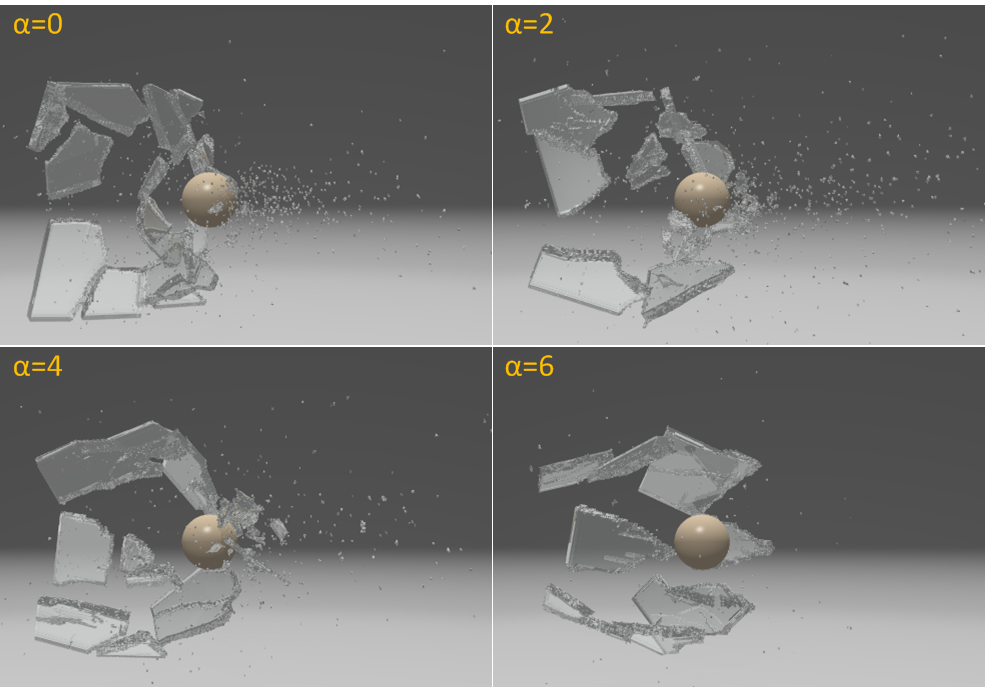
\includegraphics[width=0.6\linewidth]{chap/image/demo_shatter_control}

  \caption{\label{demo_shatter_control}
           不同 $\alpha$ 值的玻璃撞击实验。
          }
\end{figure}

\section{各向异性碎裂}
到目前为止,本文所考虑的形变和碎裂都是各向同性的,亦即材质在各个方向的动力学属性保持一致。本章节则将对本构模型进行进一步拓展,以支持各向异性的碎裂行为。具体而言,本文是通过操作粒子之间的权重函数 $\omega_{ij}$来完成的,而关键思想在于引进各向异性矩阵 $\mathbf{G}$,然后将矩阵 $\mathbf{G}$ 作用于粒子之间的 bond,从而使其在各个方向拥有不同的权重值,来简单地模拟各向异性。对于各向异性材料,权重函数 $\omega_{ij}$ 可具体写为

\begin{equation}
\omega_{ij}=\frac{\delta}{|\mathbf{G}(\mathbf{x}_j-\mathbf{x}_i)|}
\end{equation}

其中各向异性矩阵 $\mathbf{G}$ 其行列式一般为 1,即 $|\mathbf{G}| = 1$。利用这一模型,可以产生非常明显的各向异性碎裂现象。如图\ref{demo_impact_color_map} 所示。

\begin{figure}[!htb]
  \centering
  \captionsetup{justification=centering}
  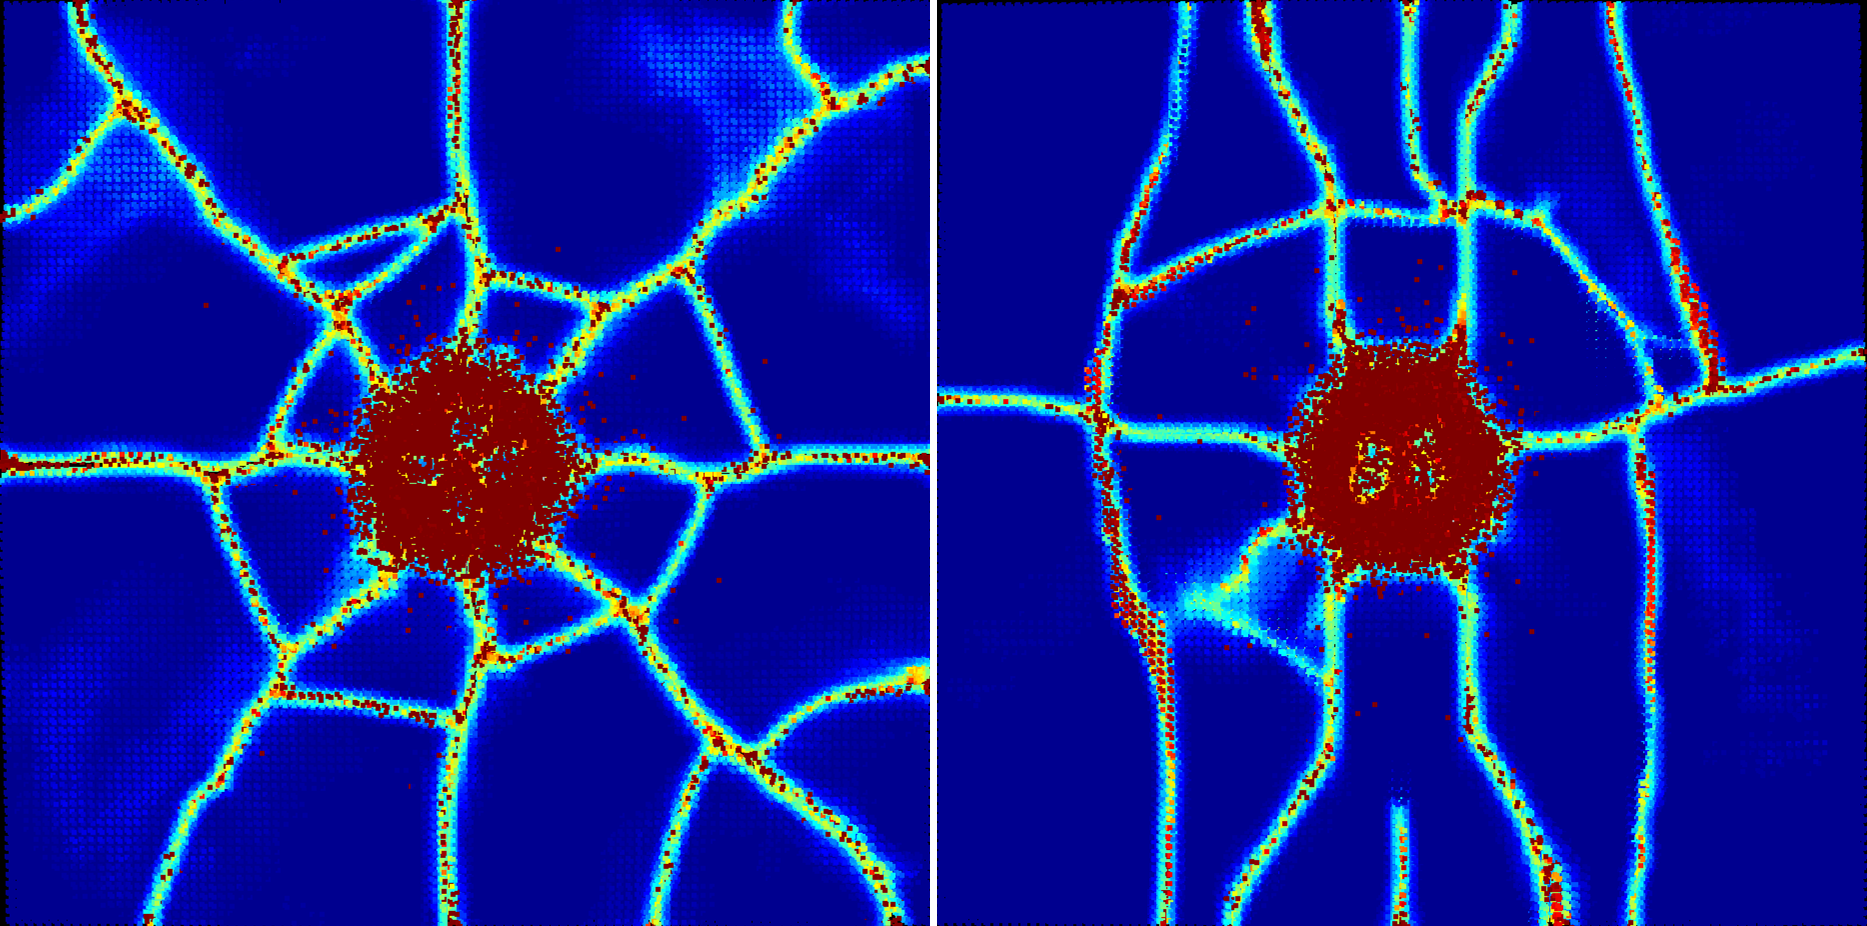
\includegraphics[width=0.6\linewidth]{chap/image/demo_impact_color_map}

  \caption{\label{demo_impact_color_map}
           各向同性碎裂(左图)和各向异性碎裂(右图)产生的碎裂模式对比。其中蓝色表示粒子未发生碎裂,而红色表示粒子已经完全发生碎裂。可以看到,在各向异性矩阵 $\mathbf{G}$ 的作用下,碎裂模式在 x,y 两个不同的方向明显不同,其中 x 方向更难发生碎裂,而 y 方向则相对更容易发生碎裂。
          }
\end{figure}

值得注意的是,事实上材质中的各向异性行为是极为复杂的,学术界也在提出不同的模型来进行解释。在本文工作中,我们仅仅是通过对权重函数来进行简单扩展,虽然取得了不错的各向异性碎裂效果,但在表达能力上仍然是有所欠缺的。现阶段关于近场动力学理论各向异性的更成熟模型仍有待探索。

\section{碎裂之拓扑更新}
\label{fracture_discretization}
在章节\ref{discretization} 中,已经详细阐述了本文工作所采用的离散化框架,以及物体形变时通过加权平均的方式来对网格顶点的位置来进行更新。但对于碎裂问题,其改变的不仅仅是顶点的位置,而是同时需要改变其拓扑连接关系,因此这一问题相对于形变要更为复杂。

为方便讨论,我们将在二维情况下进行算法阐述,但将其拓展到三维是自然的,并不存在障碍。本文工作所提出的碎裂策略受\mycite{Chen}{2013}启发,同样是采用沿四面体边缘分割的方法,不过其仅仅针对脆性材料的碎裂仿真。沿四面体边界分离的策略还类似于工作\textcolor{blue}{(M\"{u}ller et al. 2001)\parencite{Muller2001}}。本文工作所用具体算法可如下图 \ref{topology_control} 所示。

\begin{figure}[!htb]
  \centering
  \captionsetup{justification=centering}
  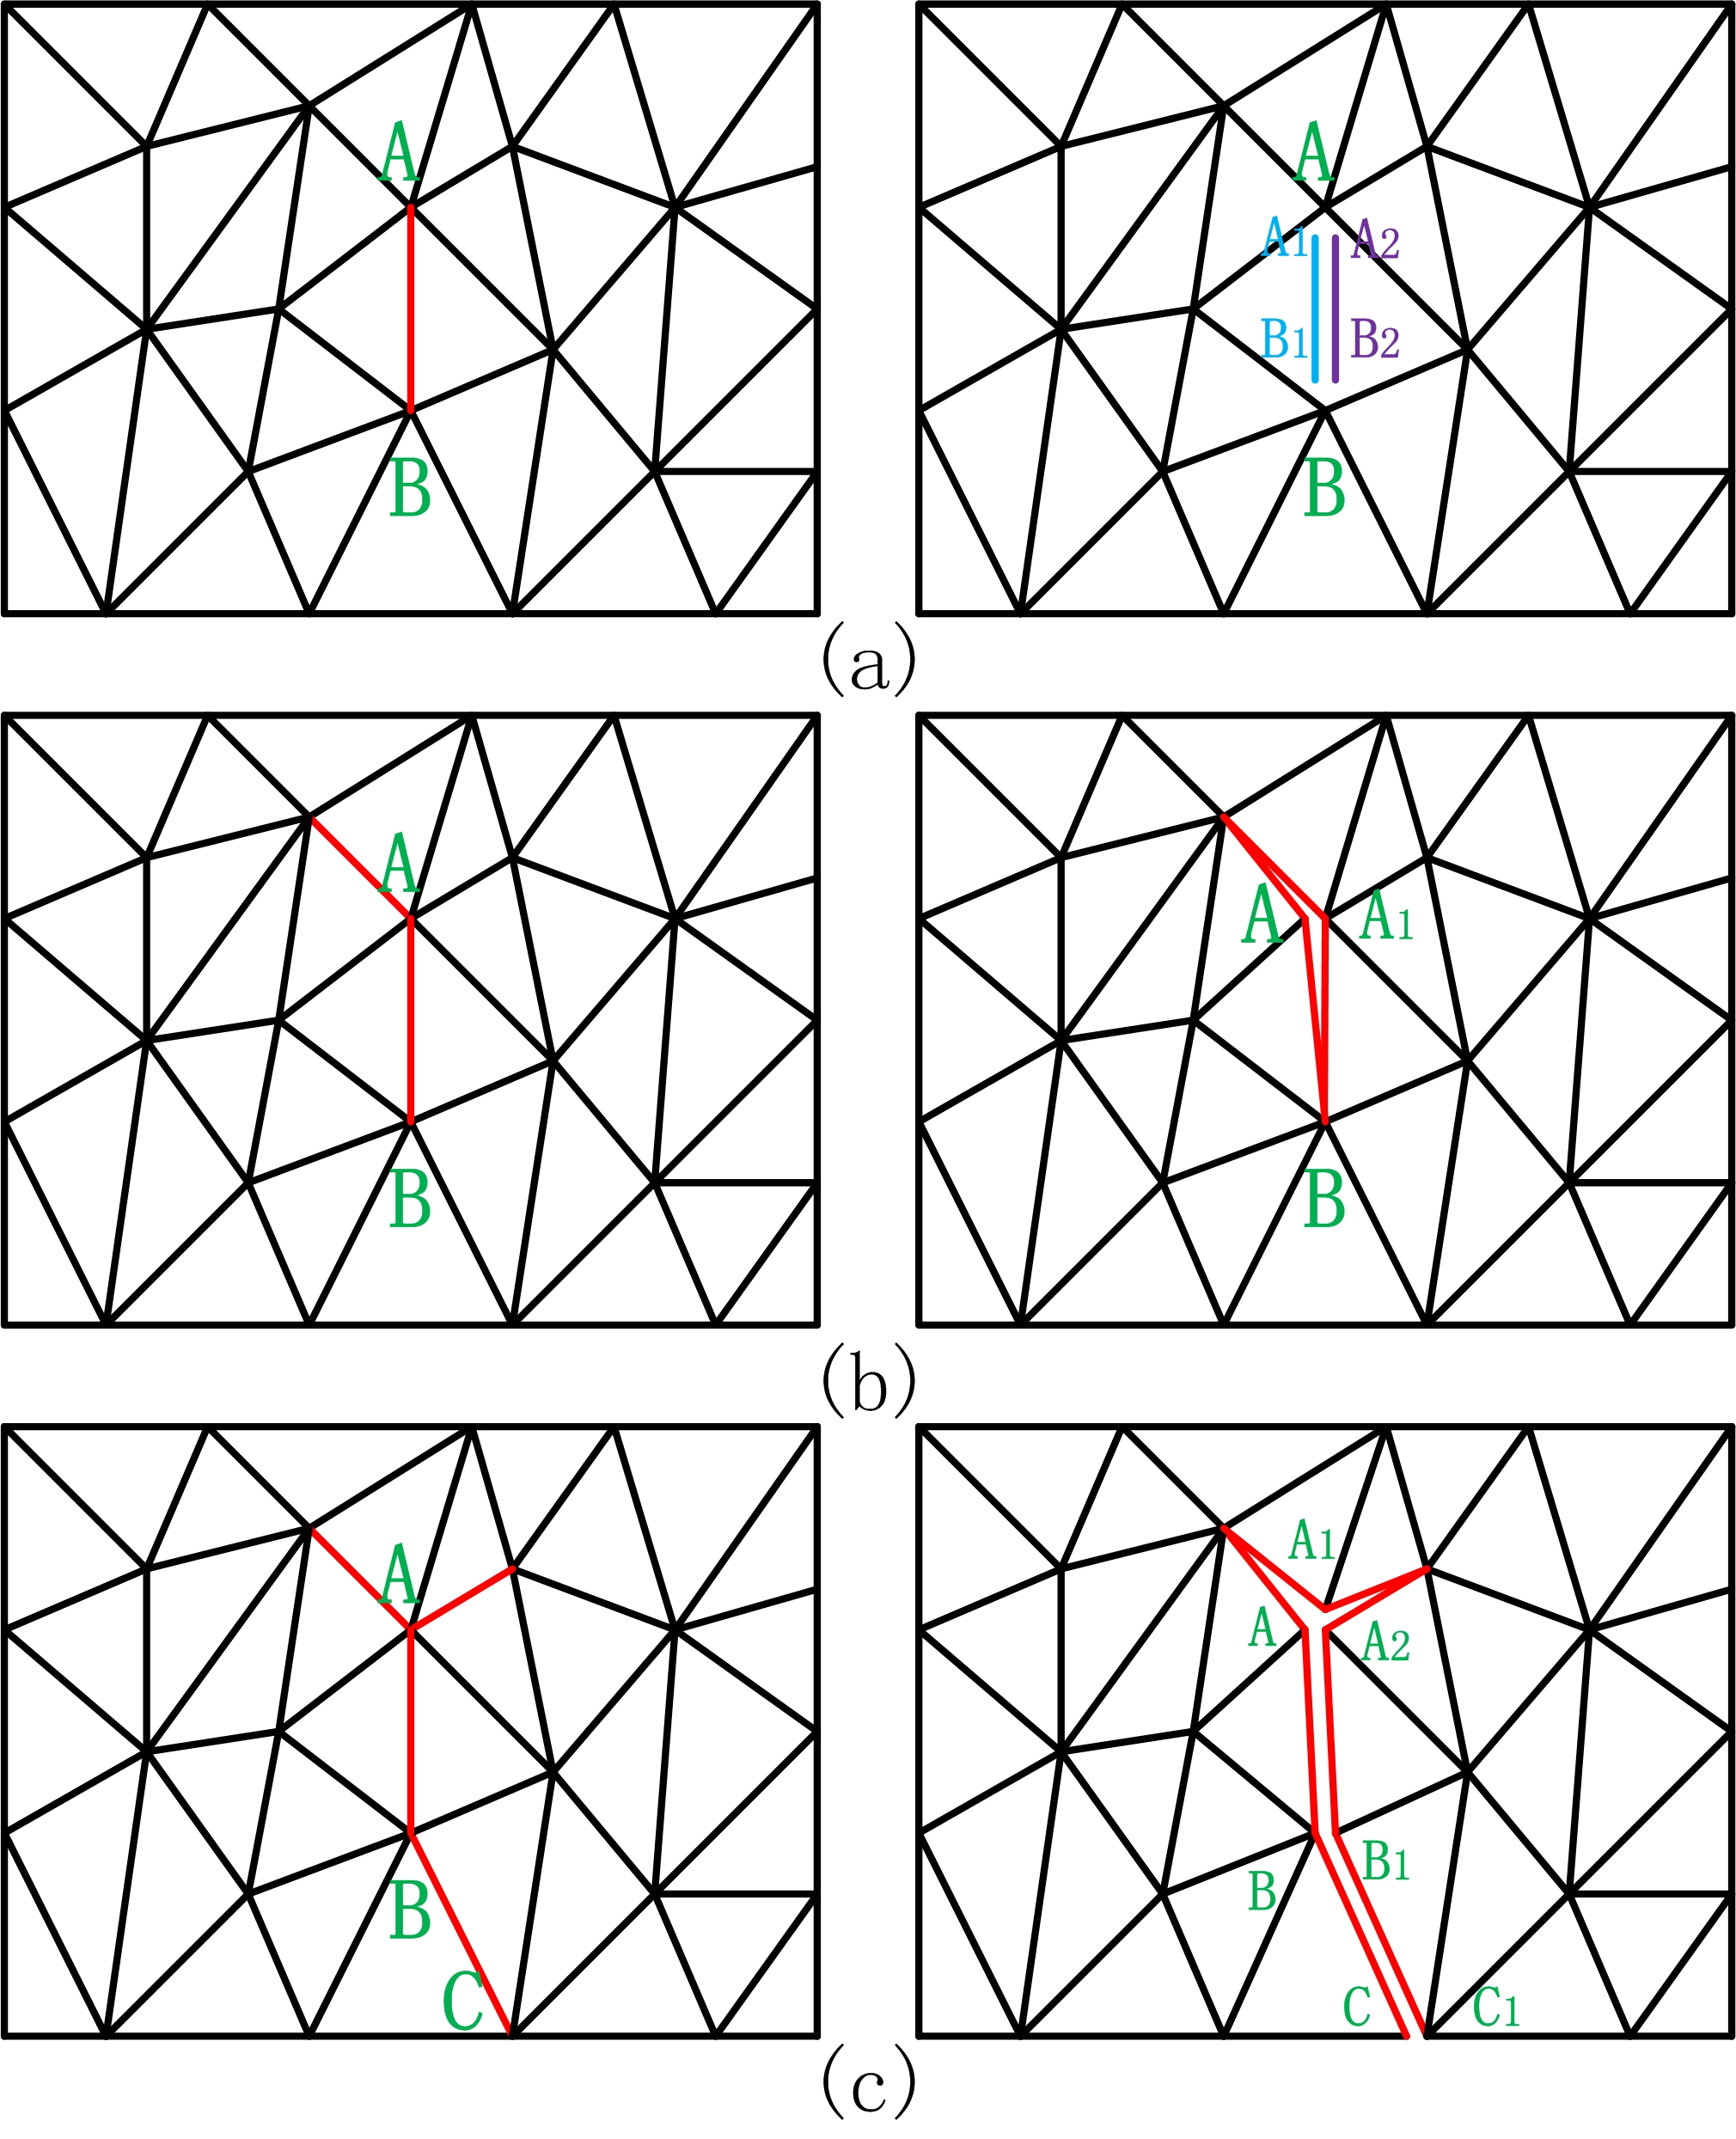
\includegraphics[width=0.6\linewidth]{chap/image/topology_control}
  \caption{\label{topology_control}
           碎裂之拓扑更新算法。图(a)表示在形变体发生碎裂时,单纯地复制碎裂边并不可取。图(b)表示将复制边策略转变为顶点分裂策略,当另一条碎裂边加入时,则可以将顶点进行分裂。图(c)表示多处同时发生碎裂。
          }
\end{figure}

如图\ref{topology_control}(a)中,当共享 AB 边的两个三角形(对应两个物理仿真粒子)发生碎裂时(三维情下对应共享面和四面体),对于脆性材料的碎裂,通常使用的策略是直接复制 AB 边,得到 $\texttt{A}_1\texttt{B}_1$ 和 $\texttt{A}_2\texttt{B}_2$。 但对于形变体的碎裂,这一策略并不可行,因为在脆性材料中可以认为这两条边是完全重合的,而在形变体中则不然,因此也无法决定使用$\texttt{A}_1$ 还是 $\texttt{A}_2$ 去替换原有顶点 A,以及使用 $\texttt{B}_1$ 还是 $\texttt{B}_2$ 去替换原有顶点 B。 为解决这一问题,我们将边复制(三维情况下对应面复制)问题转换为在 FEM 中常用的顶点分裂问题。如图\ref{topology_control} 所示,我们需要暂时推迟顶点 A 的分裂在拓扑上的反映,直到另外一条碎裂边(crack edge)加入。如此,我们便可以自然地将顶点 A 分裂成 $\texttt{A}_1$ 和 $\texttt{A}_2$,以反映碎裂引起的拓扑变化,因为此时这两条碎裂边已经将与顶点 A 相连的所有三角形隔离成不通过顶点 A 相连的两个独立部分。

在具体实现中,首先需要在仿真开始前遍历整个三角网格,并且为每个顶点存储其直接相连的三角形序号。在仿真过程中,我们仅仅需要考虑当前新产生碎裂边中所涉及的顶点,因为只有这些顶点才具有分裂的可能。对于每一个已经发生碎裂并可能需要进行分裂的顶点,我们判断与其相连的三角形是否已经被碎裂边隔离成不通过此顶点相连的两个独立部分。如果是此情形,则将顶点进行复制,并将其赋予给不同的三角形,即完成顶点的分裂过程。在顶点分裂之后,便可以将这些碎裂边进行删除,因为物体新的边界已经形成。如果与该顶点相连的三角形可以被分裂多个独立部分,则相应将顶点分裂成多份,如图\ref{topology_control}(c)所示。此外,如果同一碎裂边的多个顶点同时发生碎裂,此算法同样可以兼容。关于与顶点相连三角形的独立部分的具体查找,本文工作使用并查集 (disjoin set)算法来进行实现。

上述方法在理解上较为直观,实现上也并不复杂,并且能够取得非常逼真的视觉效果,具体详见\ref{fracture_results}章节。但值得注意的是,由于采用的是沿四面体边界分离的策略,而不是将四面体本身进行剖分,因此在碎裂过程中也容易产生不自然的锯齿形状。为缓解这一问题,本文工作的碎裂实验也往往在具有较高空间分辨率的四面体网格进行,以提供更多的几何细节。


\section{实验结果}
\label{fracture_results}
碎裂仿真实验运行环境和物体模型产生方法同形变仿真(章节\ref{deformation_results})一致。利用基于上述章节描述的碎裂模型和各向异性模型,本章节证明所提模型能够产生具有高逼真度的碎裂效果。

图\ref{demo_impact}所示为不同材质的碎撞击裂实验,其中一个球以恒定速度分别穿过各向同性的脆性材料、各向异性的脆性材料、各向同性的塑性材料和各向异性的塑性材料,这一实验充分展示了本文所提方法所具备的能力,其能够对多种不同属性的材料进行仿真。我们相信本文工作为图形学领域第一次使用基于近场动力学理论的仿真框架来模拟如此多样化材质的碎裂现象。

\begin{figure}[!htb]
  \centering
  \captionsetup{justification=centering}
  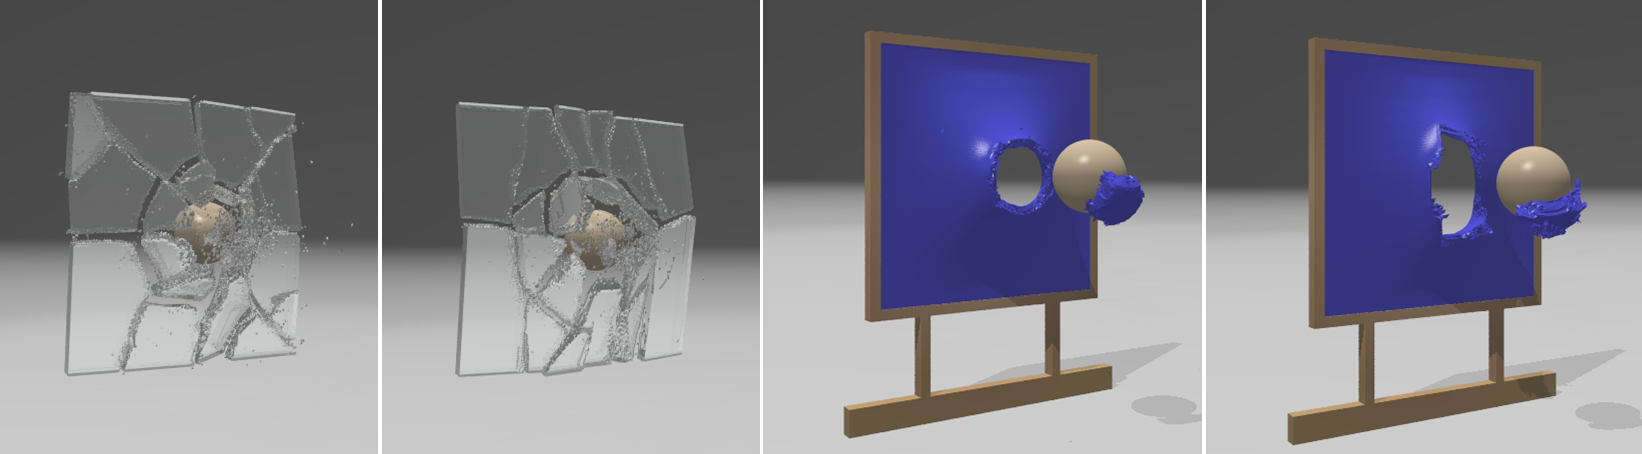
\includegraphics[width=\linewidth]{chap/image/demo_impact}

  \caption{\label{demo_impact}
           不同材质的撞击碎裂实验。球以恒定速度穿过不同材质构成的 Wall,产生不同的碎裂效果。从左到右分别为各向同性材质的脆性碎裂、各向异性材质的脆性碎裂、各向同性的塑性碎裂、各向异性的塑性碎裂。
          }
\end{figure}

图\ref{demo_impact_upside_plastic_fracture}表示具有具有不同塑性形变总量限制的可延展性碎裂实验。可以看到随着塑性总量的不同,物体的碎裂行为也有所改变。

\begin{figure}[!htb]
  \centering
  \captionsetup{justification=centering}
  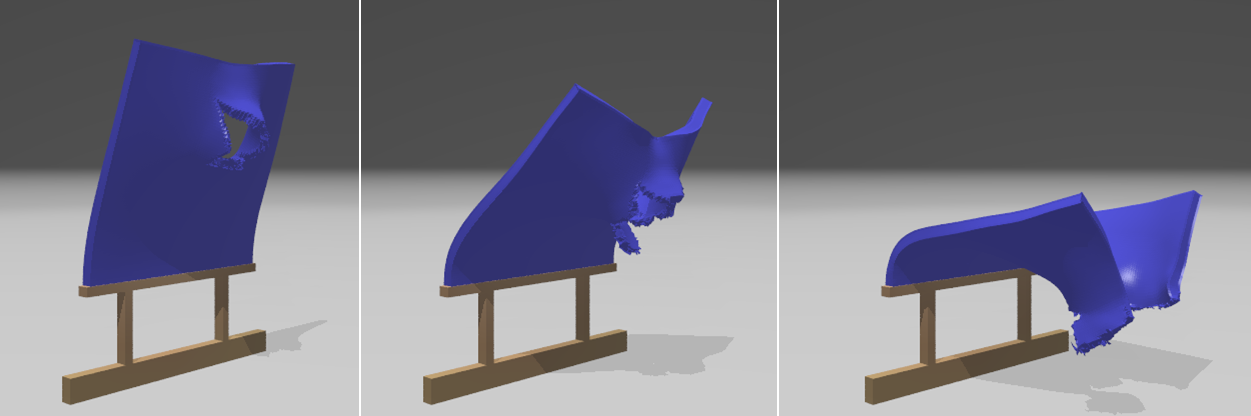
\includegraphics[width=\linewidth]{chap/image/demo_impact_upside_plastic_fracture}

  \caption{\label{demo_impact_upside_plastic_fracture}
           具有不同塑性形变总量限制的可延展性碎裂模拟,从左图到右图 $\frac{\gamma}{|\mathbf{x}_j-\mathbf{x}_i|}$ 分别为 0.1,0.15, 和 0.2.
          }
\end{figure}

图\ref{demo_tear_armadillo}展示了关于 Armadillo 的撕裂实验。仿真初始时,Armadillo 背部被固定,然后其四肢被以恒定速度撕扯,最终分离开来。这一实验充分显示本文所提方法能够仿真可延展性碎裂,以及多处同时发生的渐变式撕裂。图\ref{demo_tear_armadillo_close_view} 进一步展示了 Armadillo 撕裂实验的近视图。可以看到,当拉近摄像头时,还是可以较为明显地看出碎裂产生的锯齿状。因此,如果需要特别精细的碎裂效果,还需要更为高分辨率的物体模型,这也一定程度上说明本文方法在这一方面还存在缺陷,需要进一步改进。

\begin{figure}[!htb]
  \centering
  \captionsetup{justification=centering}
  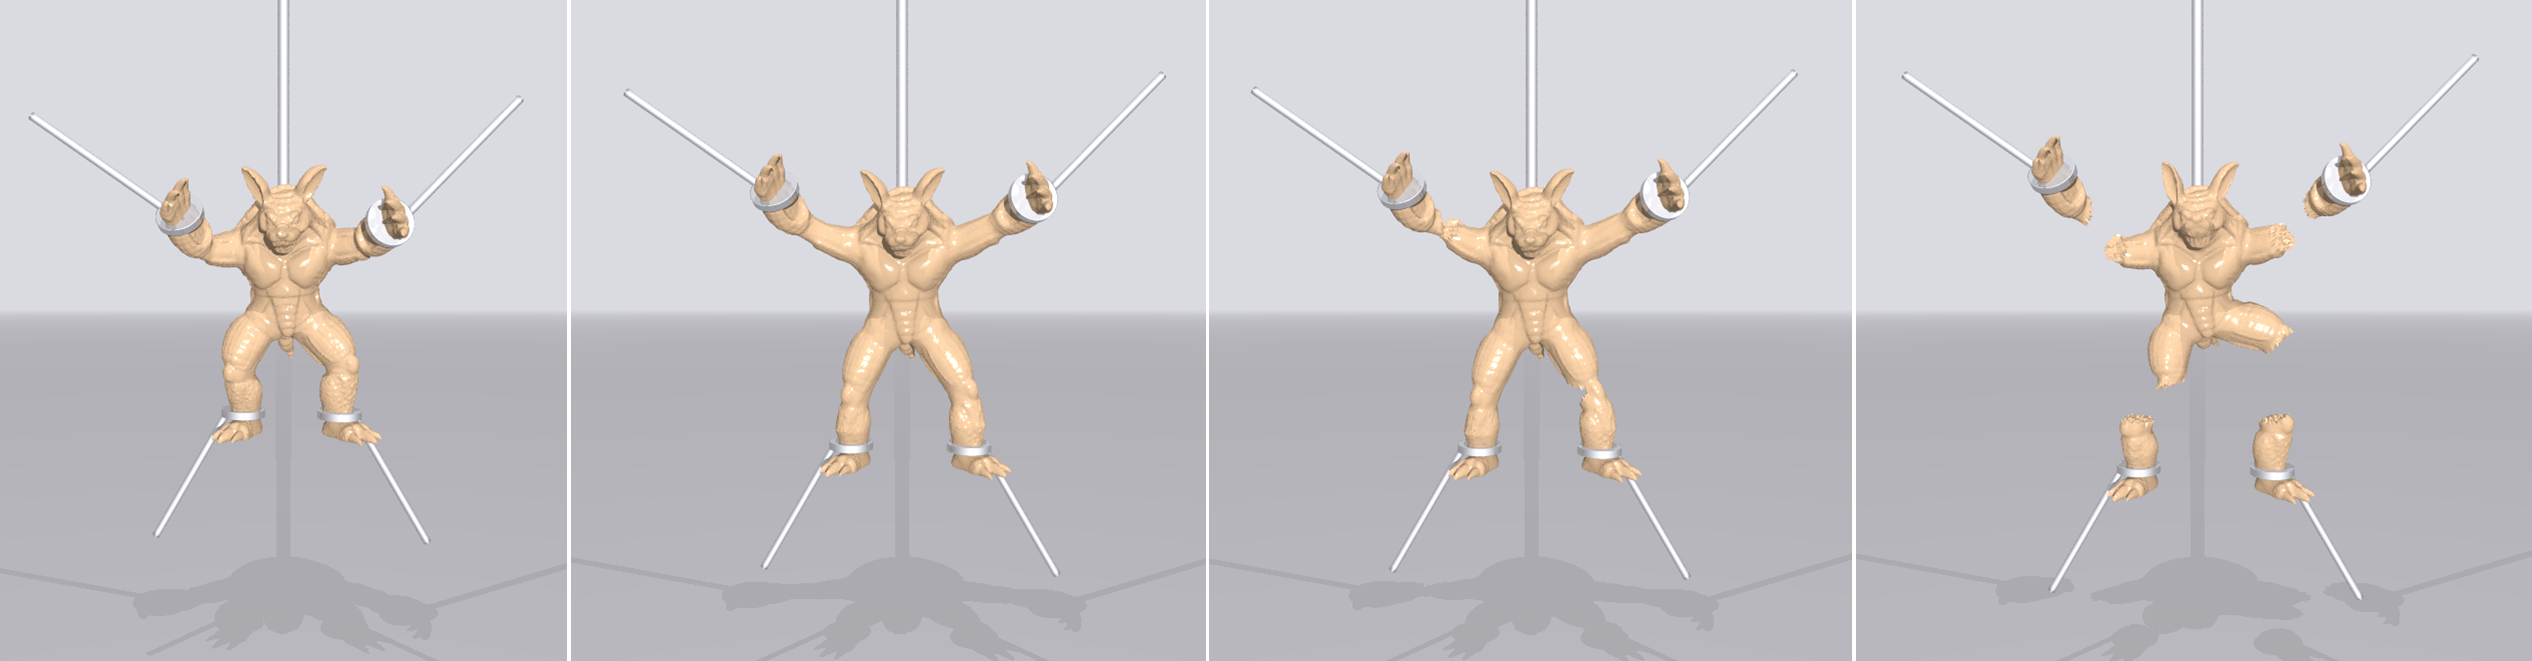
\includegraphics[width=\linewidth]{chap/image/demo_tear_armadillo}

  \caption{\label{demo_tear_armadillo}
           Armadillo 撕裂实验。Armadillo 其背部被固定,然后其四肢被撕扯裂开。
          }
\end{figure}

图\ref{demo_jello}所示为果冻穿透实验,一颗子弹以恒定速度穿过果冻,果冻被固定在地面,从而产生复杂的碎裂效果。

\begin{figure}[htbp]
\centering
\begin{minipage}[t]{0.45\textwidth}
\flushleft

  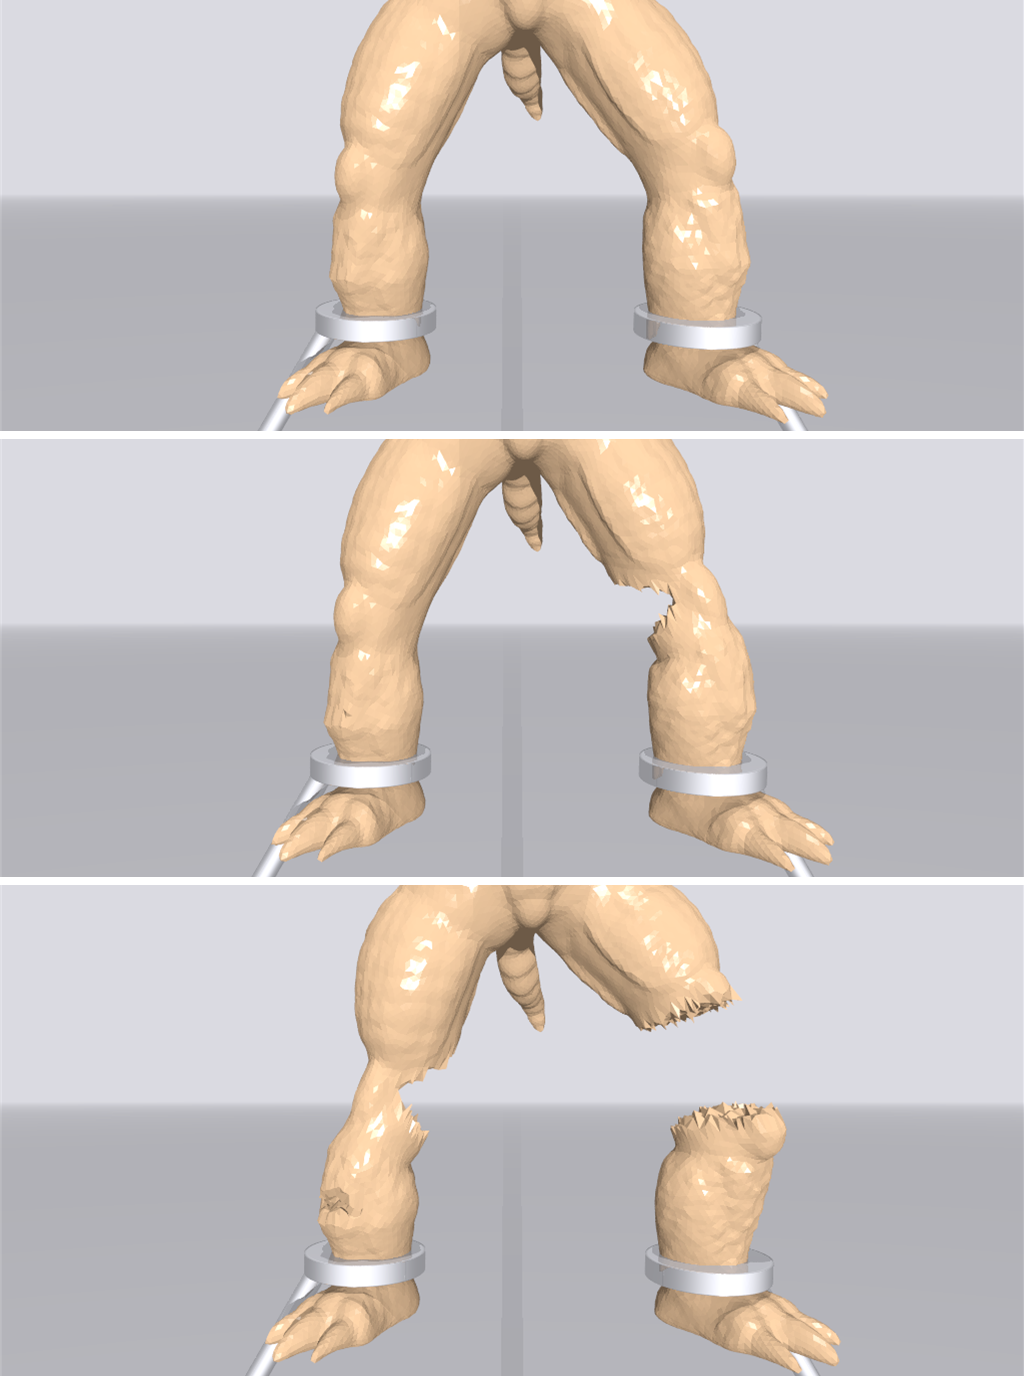
\includegraphics[width=0.9\linewidth]{chap/image/demo_tear_armadillo_close_view}
  \caption{\label{demo_tear_armadillo_close_view}
           Armadillo 撕裂实验近视图。\\从近处看,可以看到较为明显的\\锯齿状。
          }

\end{minipage}
\begin{minipage}[t]{0.45\textwidth}
\flushright

  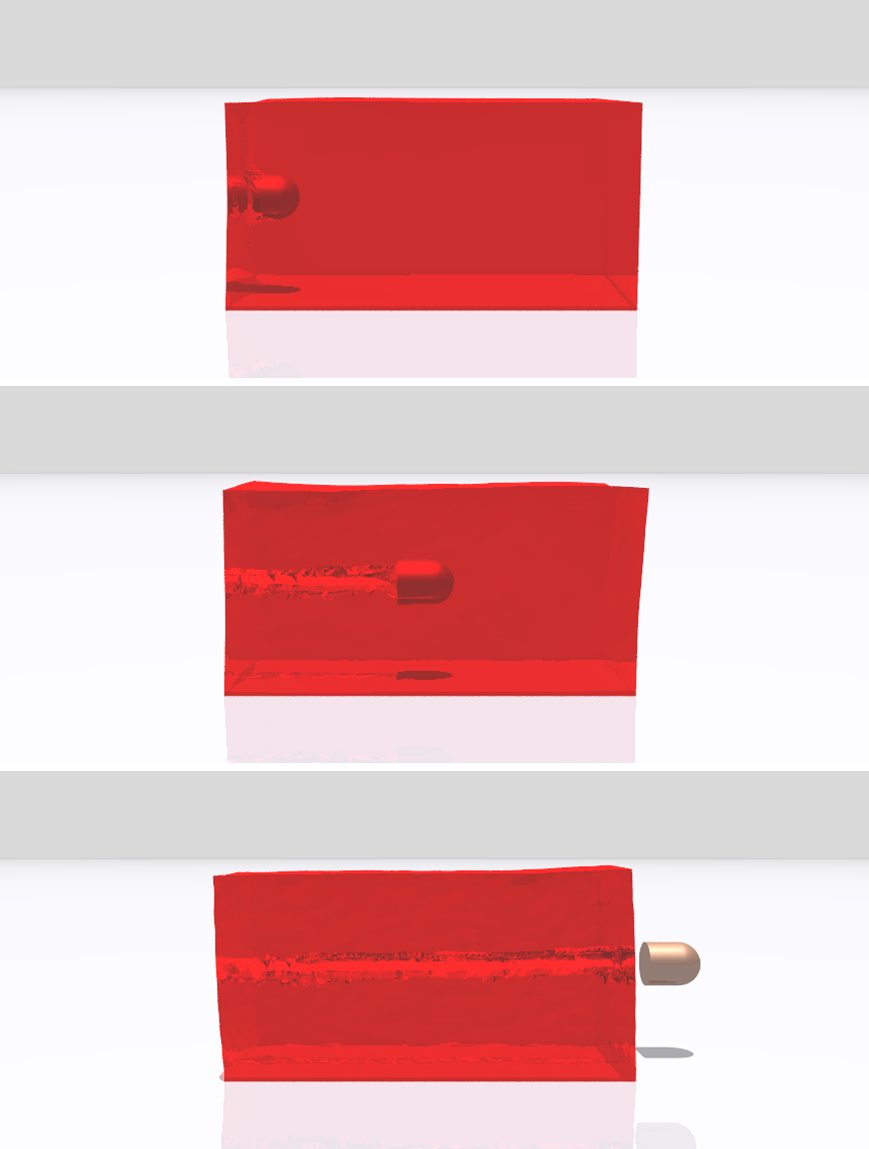
\includegraphics[width=0.9\linewidth]{chap/image/demo_jello}
  \caption{\label{demo_jello}
           果冻穿透实验。一颗子弹以恒定速度穿过果冻,产生碎裂效果。
          }

\end{minipage}
\end{figure}

图\ref{demo_brittle_fall}所示为球压玻璃板实验。玻璃板中心位置被放置一个金属球,并不断施加压力,使玻璃板发生碎裂。在这一例子中,可以清晰地看到裂纹的生长过程,效果非常惊艳。这一效果几乎不可能使用 level set 方法来实现\mycite{Hegemann}{2013},因为如此精细的裂纹需要极高空间分辨率的背景栅格。甚至对于传统 FEM 方法\textcolor{blue}{(O'Brien et al. 1999)\parencite{OBrien1999}},\textcolor{blue}{(O'Brien et al. 2002)\parencite{OBrien2002}}也是一个非常巨大的挑战,因为这一现象涉及到裂纹分支生长和合并的复杂碎裂行为,需要非常复杂 remeshing 操作。而利用本文方法,这一现象可以得到非常自然地处理。

\begin{figure}[!htb]
  \centering
  \captionsetup{justification=centering}
  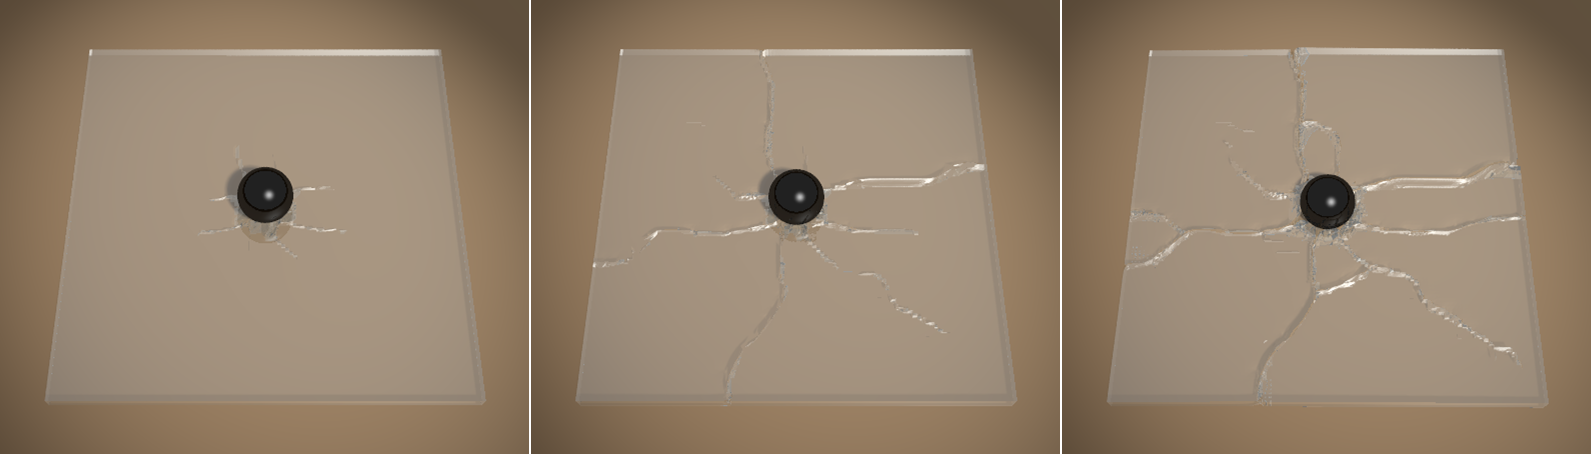
\includegraphics[width=\linewidth]{chap/image/demo_brittle_fall}

  \caption{\label{demo_brittle_fall}
           玻璃板受压实验。玻璃板中心位置被放置一个金属球,并不断施加压力,从而发生碎裂。图中可以看到明显裂纹生长过程,证明本文所提方法能够轻松处理裂纹分支的生长以及合并。
          }
\end{figure}

图\ref{demo_fall_bunny}所示为 Bunny 衰落实验。一个弹性 Bunny 摔落在地板上,并散成多块。从中可以看到本文方法的方法能够捕捉到材质的二次碎裂线性。

\begin{figure}[!htb]
  \centering
  \captionsetup{justification=centering}
  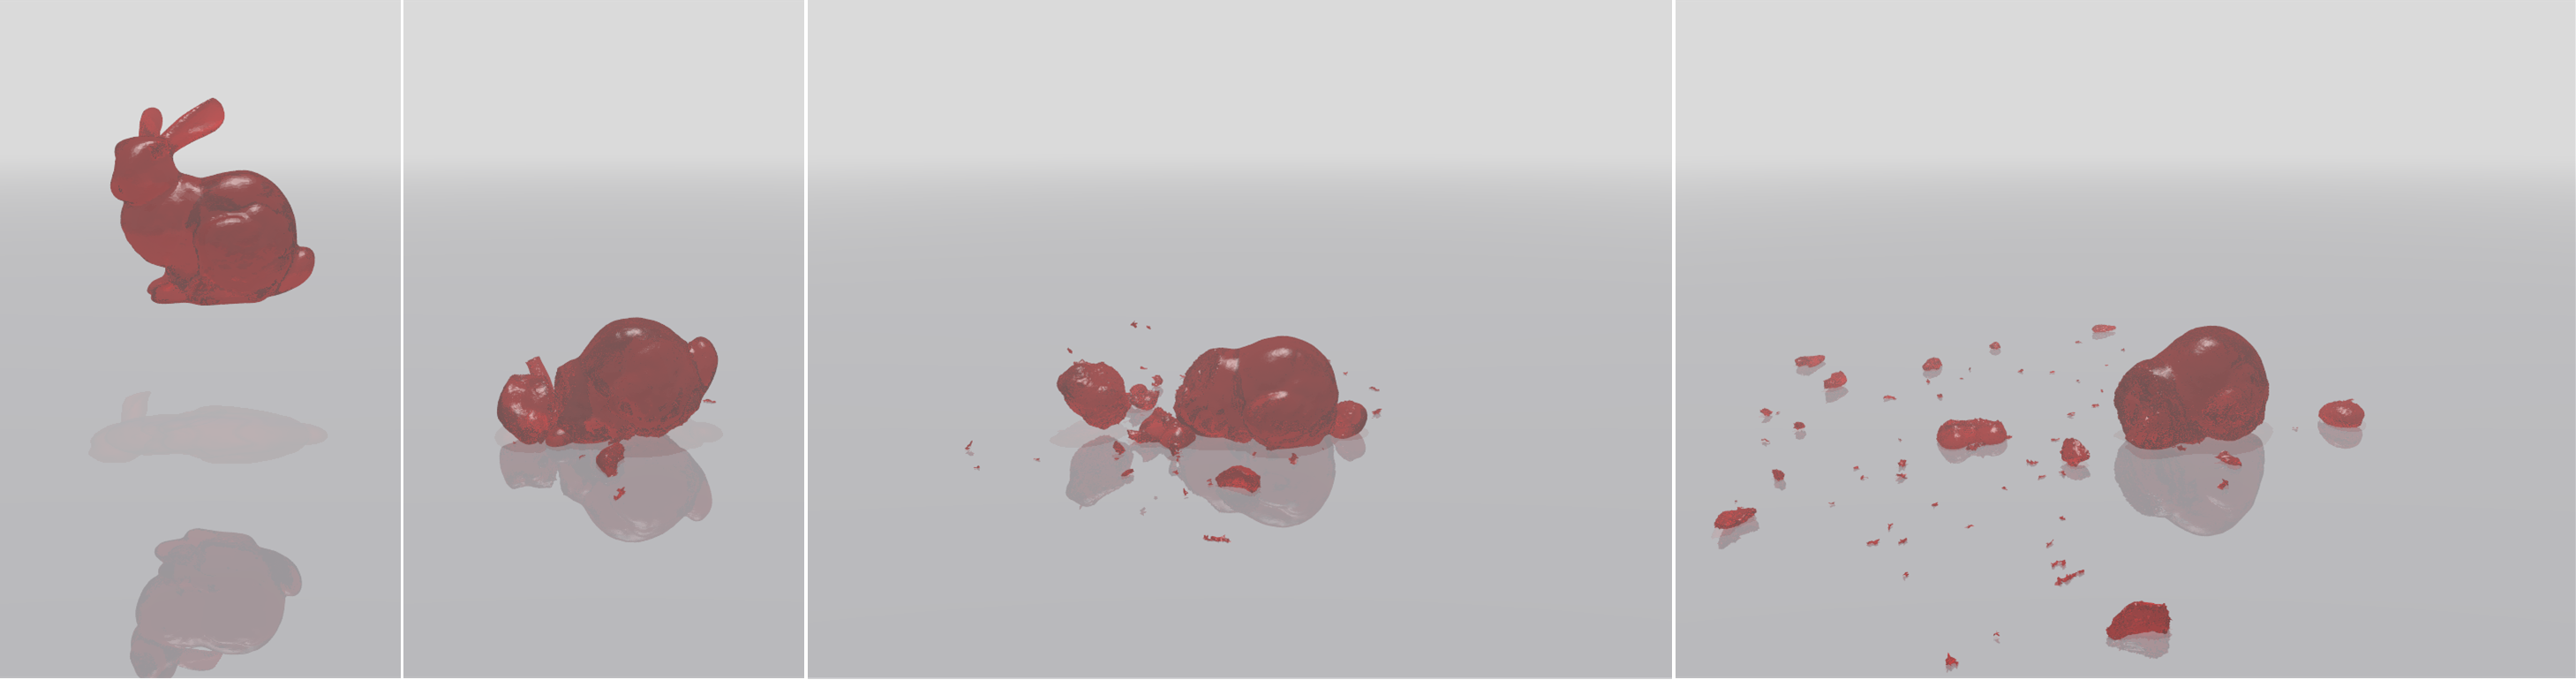
\includegraphics[width=\linewidth]{chap/image/demo_fall_bunny}

  \caption{\label{demo_fall_bunny}
           Bunny 摔落实验。一个弹性 Bunny 摔落在地板上,并散成多块。注意图中的二次碎裂效果。
          }
\end{figure}

最后一个实验为薄片撕裂实验,如图\ref{demo_tear_thin_sheet}所示。在此实验中,弹性薄片从两边进行撕扯,最开始的开裂处位于边端,但裂纹随后扩展到整块薄片,将薄片分裂成多块。注意其中由于裂纹分支以及合并而产生的丝絮状细块(filaments)。

表\ref{fracture_results_table}展示了上述碎裂仿真实验所有模型参数以及物理参数。

\newpage
\begin{figure}[!htb]
  \centering
  \captionsetup{justification=centering}
  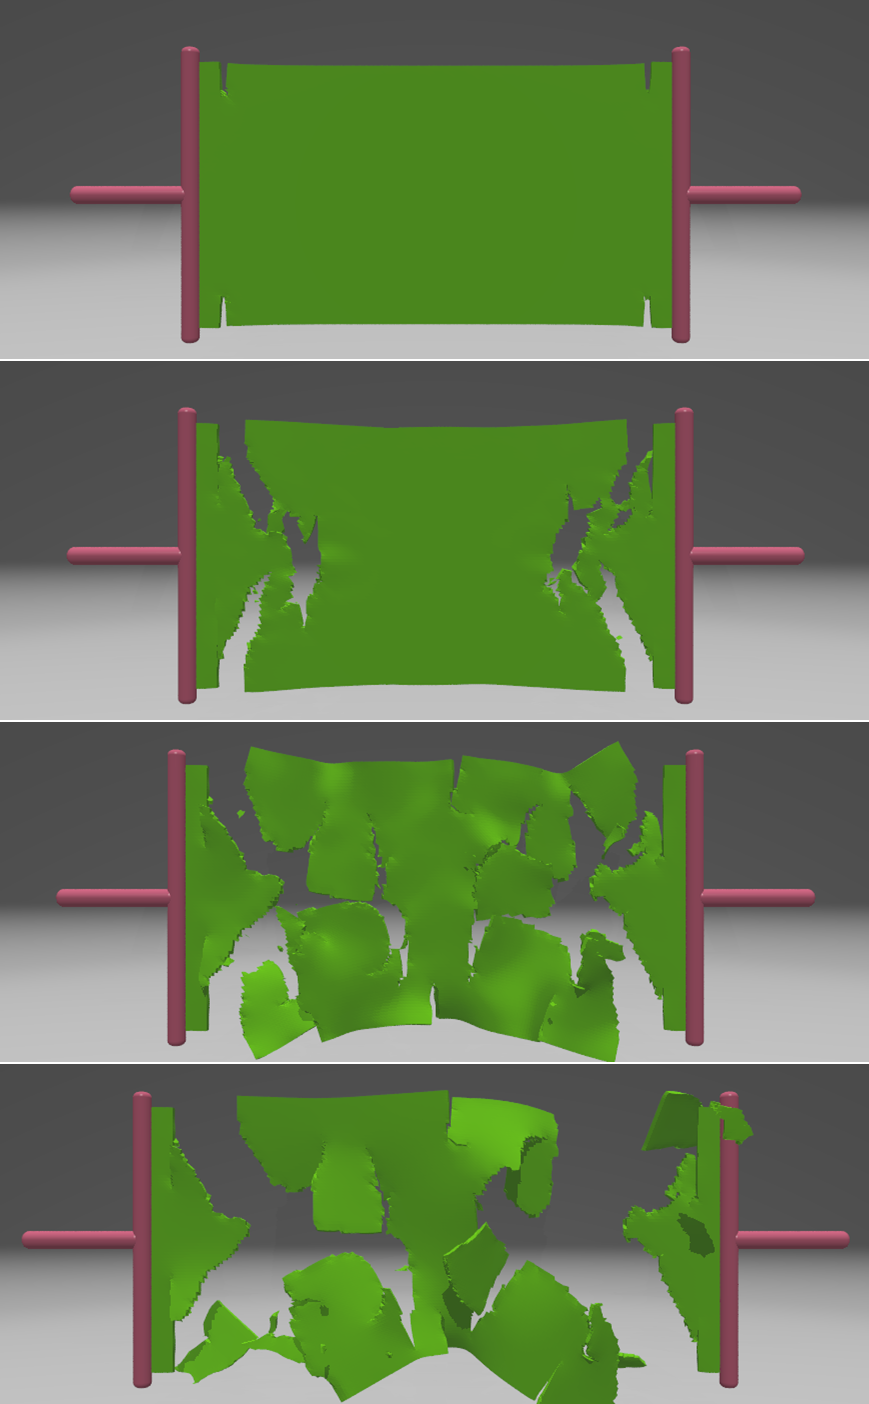
\includegraphics[width=0.6\linewidth]{chap/image/demo_tear_thin_sheet}

  \caption{\label{demo_tear_thin_sheet}
           薄片撕裂实验。薄片从两端开始撕裂,最终扩展到全部区域,注意其中的裂纹分支以及合并。
          }
\end{figure}

\begin{table*}[htb!]
\centerline{
\resizebox{1.3\textwidth}{!}{
\begin{tabular}{lccccccccccccc}
  \hline
  \hline
  Examples & particle num & $\delta$ & bond num & $\kappa$ & $\mu$ & $\rho$            & $\Psi_0$ & $\frac{\gamma}{|\mathbf{x}_j-\mathbf{x}_i|}$ & $s^w_{(k)(j)}$ & $\Delta t$ &$\lambda_a$    & $\lambda_l$  & performance\\
           &              &          &          &   (KPa)   & (KPa)  &(Kg/$\mathrm{m}^3)$&          &                                              &                & (s)       &   &   &(s/step)\\
  \hline
  Glass Wall[Figure~\ref{demo_impact}(a)(b),~\ref{demo_brittle_fall}]     & $3.0\times10^5$ & 1.45$\lambda$ & $5.0\times10^7$ & $3.3\times10^{7}$ & $2.0\times10^{7}$        & 2200 & $\infty $ & 0.0             & 0.0005   & $1.0\times10^{-6}$          &0&0& $\sim2.4$ \\
  Plastic Wall [Figure~\ref{demo_impact}(c)(d)]  & $3.0\times10^5$ & 1.45$\lambda$ & $5.0\times10^7$ & $3.3\times10^{3}$ & $2.0\times10^{3}$        & 2200 & $10^{25}$ & 0.2             & 0.05     & $1.0\times10^{-4}$          &$0.002$&0& $\sim2.4$ \\
  Wall [Figure~\ref{demo_impact_upside_plastic_fracture}]                & $3.0\times10^5$ & 1.45$\lambda$ & $5.0\times10^7$ & $1.0\times10^{4}$ & $6.0\times10^{3}$        & 1200 & $10^{26}$ &$(0.1,0.15,0.2)$ & 0.1  & $5.0\times10^{-5}$   &0.0005&0& $\sim2.4$ \\
  Jello [Figure~\ref{demo_jello}]               & $4.6\times10^5$ & 1.45$\lambda$ & $8.6\times10^7$ & $1.0\times10^3$   & $4.6\times10^2$          & 1000 & $\infty $ & 0.0             & 0.4      & $5.0\times10^{-5}$   &0&0& $\sim3.8$ \\
  Armadillo [Figure~\ref{demo_tear_armadillo}]          & $4.2\times10^5$ & 1.50$\lambda$ & $7.5\times10^7$ & $6.3\times10^4$   & $3.8\times10^4$          & 1000 & $\infty $ & 0.0             & 0.61     & $1.0\times10^{-4}$          &0&0.001& $\sim5.3$ \\
  Bunny [Figure~\ref{demo_fall_bunny}]              & $5.2\times10^5$ & 1.45$\lambda$ & $8.8\times10^7$ & $2.5\times10^2$   & $1.2\times10^2$          & 1000 & $\infty $ & 0.0             & 0.13     & $5.0\times10^{-4}$          &0&0& $\sim5.2$ \\
  Thin Sheet [Figure~\ref{demo_tear_thin_sheet}]              & $1.6\times10^5$ & 1.45$\lambda$ & $2.0\times10^7$ & $5.0\times10^3$   & $3.0\times10^3$          & 1000 & $\infty $ & 0.0             & 0.1     & $5.0\times10^{-5}$          &0&0.001& $\sim1.8$ \\
  \hline
\end{tabular}
}}
\caption{碎裂仿真中的模型参数、仿真参数、及效率数据。其中 $\lambda$ 是四面体网格的平均边长度,用于邻域的初始化。}
\label{fracture_results_table}
\end{table*}


\newpage
\section{本章小结}
本章主要研究基于近场动力学方法的弹塑性碎裂模拟。第一节给出了全文工作所用的碎裂模型,我们的模型主要基于 critical stretch,但对其进行了重要改进。本章第二节随即对原有的弹塑性本构模型作了重要的拓展,引入各向异性矩阵以支持各向异性碎裂现象的模拟。第三节则重点介绍了在章节\ref{discretization}所述离散化框架的基础上,如何对拓扑结构进行更新,以在几何上反映材料的损伤,而基本思想是将面复制策略转变为顶点分裂策略。本章第四节则展示了本文方法所取得的效果。从实验结果来看,本文所提出模型能够较好地模拟弹塑性和各向异性材料的碎裂行为,并且能够很好地捕捉裂纹分支的生长以及合并现象。

    \chapter{工作总结与展望}
\section{工作总结}
本文重点对计算机图形学领域的弹塑性材料的形变仿真和碎裂仿真进行研究,并提出了一整套基于近场动力学理论的无网格仿真框架。实验结果证明,利用本文所述的弹塑性本构模型、碎裂模型、以及嵌网格策略,能够高逼真度地对物质的弹性形变、塑性形变、脆性碎裂、弹性碎裂、塑性碎裂、和各向异性碎裂进行仿真。回顾本文,主要工作在于以下几个方面:

\begin{itemize}
  \item 在第二章中,本文对于物理仿真的基本原理和碎裂仿真的基本流程进行概述性的解释,并对本构模型、碎裂模型、离散时间积分等重要模块进行介绍。本章的关键还在于详细阐述近场动力学理论的基本特性和本构方程具体形式,并对从经典连续介质力学到近场动力学的模型演变进行了详细的推导,给出了本文所用动力学模型的基本形式。
  \item 本文第三章主要研究基于近场动力学理论的形变仿真。此章首先对动力学模型进行整理,以更具物理直观的形式重新表述弹性模型。随后,本文给出了全文工作所用塑性模型,整个模型类似于经典理论中的 von Mises 模型,并对其进行改进以获的对于塑性形变的更大控制能力以及提高仿真的整体稳定性。同时,第三章还给出了全文工作所用的离散化框架,我们将粒子置于四面体网格的中心,并通过加权平均的方式来更新网格顶点位置。实践证明,基于上述模型的仿真算法能够对物质的弹塑性行为进行高逼真地仿真。和 FEM 的对比实验也证明,本文工作所用的算法在效果上能够达到和 FEM 共旋线性模型几乎一致的效果。
  \item 本文第四章建立在第三章基础之上,主要研究基于近场动力学理论的碎裂仿真。全章首先描述了全篇工作所用的碎裂模型,本文所用碎裂模型基本上基于 critical stretch,但对其进行了两点重要改进。第一是再次引入权重函数 $\omega_{ij}$,避免离中心粒子越近的邻域粒子反而容易发生断裂。第二是随着碎裂的进行,持续提高碎裂的门槛,以防止产生过多的小碎块。随后,此章还重点介绍了在第三章离散框架基础上,如何进行拓扑更新,以反映碎裂引起的分裂行为。利用上述模型,本文进行了大量的实验工作,并且证明所提框架能够对物质的弹性脆裂、脆性碎裂、塑性碎裂、各向异性碎裂进行准确仿真,同时还能方便处理材料的二次碎裂以及裂纹分支的生长和合并行为。
\end{itemize}

\section{未来展望}
本文对基于近场动力学理论的弹塑性形变和碎裂进行了研究和探讨,并取得了一定的研究成果,但同时也存在诸多不足和亟待完善之处。在此,本文列出这些需要待完善的部分以及其他有意义的研究方向,作为对未来工作的展望。

\begin{itemize}
  \item 碎裂模型及离散化框架的进一步改进。受限于碎裂模型,当前离散化框架将物体仿真粒子置于四面体网格的中心,并沿着单元体边界而进行分裂。虽然处理方便并且取得了不错的效果,但仍需要空间分辨率较高的仿真网格来增加碎裂细节,否则将会产生较为明显的锯齿效果。因此,更实用的离散框架仍然是将仿真粒子直接对应到网格顶点,然后使用基于类似 FEM 中顶点分裂的方式直接对四面体进行剖分。但在近场动力学框架中,这同时需要提出全新的基于粒子而不是如当前基于 bond 的碎裂模型。如果能够提出合适的碎裂模型,则可以结合 FEM 方法中对于拓扑表示的优点以及近场动力学在物理计算上的有点,更为逼真地仿真碎裂行为。
  \item 近场动力学的隐式时间积分算法。在章节\ref{elasitcity_model}中我们指出,近场动力学的隐式积分算法相对于传统模型要更为复杂,这是由于其理论的非局域性引起的,粒子之间的力计算和整个邻域内的其他粒子相关。如果能够提出对于 state based 模型的高效隐式时间积分算法,对于进一步挖掘近场动力学的潜力,具有重要意义。
  \item 基于GPU的并行实现。当前的实现采用基于 openMP 的多线程 CPU 并行,但近场动力学模型本身特别适于并行化,因此更高效率的方式是基于 GPU 的并行框架来进行实现,相对于 CPU 实现,在效率上应该能大幅提升。
  \item FEM 和近场动力学方法的耦合。可以将这两种方法进行耦合,在缺陷之处进行彼此弥补,并同时发挥两者的优势。
\end{itemize}
    


	\appendix
	\printbibliography[heading = bibintoc]

	\backmatter
	\chapter{致谢}
感谢我的导师李胜副教授。李老师是我从天体物理转向计算机图形学方向的领路人,无论是在学术上还是人生道路上,都给予了我很大帮助。感谢汪国平教授,其工作态度永远值得我们学习。

感谢朱飞师兄,没有朱飞师兄对我的提携和不断督促,以及对本工作的不断完善,本工作将是错漏百出、举步维艰的。感谢何小伟师兄、杨升师兄、徐力有师弟、朱奎鑫师弟、田然师弟在科研讨论时提供的有效思路及帮助。

感谢北京大学,从本科到硕士,度过了我最为美好、最为充实的七年时光。

最后,感谢那些还陪伴在我身边的人以及未来会陪伴在我身边的人,你们的存在是我不断努力、奋勇向前的最大动力与意义。

人生但苦无妨。未来,愿付出所有,换前所未有。

    \chapter{攻读硕士学位期间取得成果}

\noindent{\textbf{论文}}
\begin{itemize}
  \item \textbf{Wei Chen}, Fei Zhu, Jing Zhao, Sheng Li, Guoping Wang. Peridynamics-Based Fracture Animation for Elastoplastic Solids. Computer Graphics Forum, Volume37, Issue1 February 2018, Pages 112-124.
\end{itemize}

\vspace*{5cm}

\noindent{\textbf{参与项目}}
\begin{itemize}
  \item 开源物理引擎 Physika
  \item 2017-2022: 复杂时变场景的物理仿真关键技术\\
  (国家重点研发计划项目)
  \item 2017-2022: 基于动力学的视觉特效并行模拟技术和引擎\\
  (国家重点研发计划项目)
\end{itemize}

	% Copyright (c) 2008-2009 solvethis
% Copyright (c) 2010-2017 Casper Ti. Vector
% All rights reserved.
%
% Redistribution and use in source and binary forms, with or without
% modification, are permitted provided that the following conditions are
% met:
%
% * Redistributions of source code must retain the above copyright notice,
%   this list of conditions and the following disclaimer.
% * Redistributions in binary form must reproduce the above copyright
%   notice, this list of conditions and the following disclaimer in the
%   documentation and/or other materials provided with the distribution.
% * Neither the name of Peking University nor the names of its contributors
%   may be used to endorse or promote products derived from this software
%   without specific prior written permission.
%
% THIS SOFTWARE IS PROVIDED BY THE COPYRIGHT HOLDERS AND CONTRIBUTORS "AS
% IS" AND ANY EXPRESS OR IMPLIED WARRANTIES, INCLUDING, BUT NOT LIMITED TO,
% THE IMPLIED WARRANTIES OF MERCHANTABILITY AND FITNESS FOR A PARTICULAR
% PURPOSE ARE DISCLAIMED. IN NO EVENT SHALL THE COPYRIGHT HOLDER OR
% CONTRIBUTORS BE LIABLE FOR ANY DIRECT, INDIRECT, INCIDENTAL, SPECIAL,
% EXEMPLARY, OR CONSEQUENTIAL DAMAGES (INCLUDING, BUT NOT LIMITED TO,
% PROCUREMENT OF SUBSTITUTE GOODS OR SERVICES; LOSS OF USE, DATA, OR
% PROFITS; OR BUSINESS INTERRUPTION) HOWEVER CAUSED AND ON ANY THEORY OF
% LIABILITY, WHETHER IN CONTRACT, STRICT LIABILITY, OR TORT (INCLUDING
% NEGLIGENCE OR OTHERWISE) ARISING IN ANY WAY OUT OF THE USE OF THIS
% SOFTWARE, EVEN IF ADVISED OF THE POSSIBILITY OF SUCH DAMAGE.

{
	\ctexset{section = {
		format+ = {\centering}, beforeskip = {40bp}, afterskip = {15bp}
	}}

	% 学校书面要求本页面不要页码,但在给出的 Word 模版中又有页码且编入了目录。
	% 此处以 Word 模版为实际标准进行设定。
	\specialchap{北京大学学位论文原创性声明和使用授权说明}
	\mbox{}\vspace*{-3em}
	\section*{原创性声明}

	本人郑重声明:
	所呈交的学位论文,是本人在导师的指导下,独立进行研究工作所取得的成果。
	除文中已经注明引用的内容外,
	本论文不含任何其他个人或集体已经发表或撰写过的作品或成果。
	对本文的研究做出重要贡献的个人和集体,均已在文中以明确方式标明。
	本声明的法律结果由本人承担。
	\vskip 1em
	\rightline{%
		论文作者签名:\hspace{5em}%
		日期:\hspace{2em}年\hspace{2em}月\hspace{2em}日%
	}

	\section*{%
		学位论文使用授权说明\\[-0.33em]
		\textmd{\zihao{5}(必须装订在提交学校图书馆的印刷本)}%
	}

	本人完全了解北京大学关于收集、保存、使用学位论文的规定,即:
	\begin{itemize}
		\item 按照学校要求提交学位论文的印刷本和电子版本;
		\item 学校有权保存学位论文的印刷本和电子版,
			并提供目录检索与阅览服务,在校园网上提供服务;
		\item 学校可以采用影印、缩印、数字化或其它复制手段保存论文;
		\item 因某种特殊原因需要延迟发布学位论文电子版,
			授权学校在 $\Box$\nobreakspace{}一年 /
			$\Box$\nobreakspace{}两年 /
			$\Box$\nobreakspace{}三年以后在校园网上全文发布。
	\end{itemize}
	\centerline{(保密论文在解密后遵守此规定)}
	\vskip 1em
	\rightline{%
		论文作者签名:\hspace{5em}导师签名:\hspace{5em}%
		日期:\hspace{2em}年\hspace{2em}月\hspace{2em}日%
	}

	% 若需排版二维码,请将二维码图片重命名为“barcode”,
	% 转为合适的图片格式,并放在当前目录下,然后去掉下面 2 行的注释。
	%\vfill\noindent
	%\includegraphics[height = 5em]{barcode}
}

% vim:ts=4:sw=4


\end{document}
